\documentclass{article}
\usepackage{amsmath}
\usepackage{amssymb}
\usepackage{amsthm}
\usepackage[hidelinks]{hyperref}
\usepackage[parfill]{parskip}
\usepackage[autostyle, english = american]{csquotes} 
\MakeOuterQuote{"}

\theoremstyle{definition}
\newtheorem{theorem}{Theorem}[section]
\newtheorem{definition}[theorem]{Definition}

\DeclareMathOperator{\ord}{ord}
\DeclareMathOperator{\dl}{dl}

%Domande nei vari appelli
% 2024
%	MLP
%	Fuzzy set
%	Evolutionary algorithms
%
%	Som: definizione, algoritmi di configurazione e operazioni
%	Fuzzy Controller System (control method e operazioni)
%	Intelligenza di Sciame (Swarm Colony Optimization e Ant Colony Optimization)
%
%	MLP
%	Fuzzy control
%	Swarm intelligence
%
%	Radial Basis Function Networks
%	Fuzzy Sets: definitions, membership fn and operations 
%	Evolutionary Algorithms for multi-criteria optimization
%
%	recurrent networks
%	fuzzy sets
%	swarm intelligence
%
%	Hopfield Networks
%	Data Analysis: Fuzzy Clustering, extensions
%	EAs, coding chromosomes, fitness, selection, genetic operators
%
% 2025
%	RBFN
%	Fuzzy controller (modeling/operations)
%	EA: chromosome encoding, fitness, operators (mutual/crossover), selection
%
%	Mlp
%	fuzzy data analysis
%	Swarm

\begin{document}
	
	\title{AI Summary}
	\author{Massimo Perego}
	\date{}
	\maketitle
	
	\tableofcontents
	
	\newpage
	
	%%%%%%%%%%%%%%%%%%%%%%%%%%%%%%%%
	% Domande sulla prima parte:
	% x	MLP 
	% x	RBFN
	% x	LVQN
	% X	SOM
	% X	Hopfield
	% X	Boltzmann machines
	% X	Recurrent
	%%%%%%%%%%%%%%%%%%%%%%%%%%%%%%%%
	
	\section{Neural Networks}

\subsection{Biological Background}
\textbf{Neural Networks} need a biological introduction since they're \textbf{inspired from the human brain}, neurons in the network are simplified versions of the human neurons.\\

The human brain is studied in multiple different fields various reasons, in Computer Science the objective of studying the brain is \textbf{mimicking certain cognitive capabilities} of human beings, with the \textbf{objective} of \textbf{solving} learning/adaptation, prediction and optimization \textbf{problems}.\\

But why? Neural networks in Artificial intelligence allow for \textbf{highly parallel information processing}.\\

Neurons have a \textbf{cell body}, called \textbf{soma}, from which extend several \textbf{short ramified branches} called \textbf{dendrites} and a \textbf{long extension} called \textbf{axon}; at its end the axon is heavily ramified.\\

The axons are fixed paths along which neurons communicate with each other; the axon of a neuron leads to the dendrites of another. The place in which an axon and a dendrite almost touch each other is called \textbf{synapse}.\\

A terminal button of the axon releases \textbf{neurotransmitters} that act on the membrane of the receiving dendrite, changing its polarization.\\
Synapses that reduce the potential difference are called \textbf{excitatory}, those that increase it are called \textbf{inhibitory}.\\

If there is enough net excitatory input the \textbf{axon is depolarized} (the potential difference is significantly reduced), the cell is "activated", the change in electrical potential is propagated to another cell, where the process is repeated; when this action potential reaches the terminal buttons, neurotransmitters are released.\\

Changes in electrical potential are accumulated at the cell body of a neuron and, if they reach a certain threshold, are propagated along the axon.\\

Synapses are what enables parallel information to travel, a single neuron can activate multiple synapses and activate many more neurons, permitting complex reasoning.\\

\textbf{Advantages} of \textbf{Neural Networks}:
\begin{itemize}
	\item \textbf{High processing speed} due to massive parallelism given by large number of neurons (in CS implemented by CUDA architectures)
	
	\item \textbf{Fault Tolerance}: remain functional even if some parts of a network get damaged; if a neuron goes crazy the rest will still function, even if a little bit worse
	
	\item \textbf{"Graceful Degradation"}: gradual degradation of performance if an increasing number of neurons fails (consequence of the fault tolerance)
	
	\item \textbf{Well suited for inductive learning} (learning from examples, generalizing from instances, usually the point of a neural network is to have some examples and generalize from there)
\end{itemize}

It appears to be reasonable to try \textbf{mimicking or to recreate these advantages by constructing artificial neural networks}.
\begin{center}
	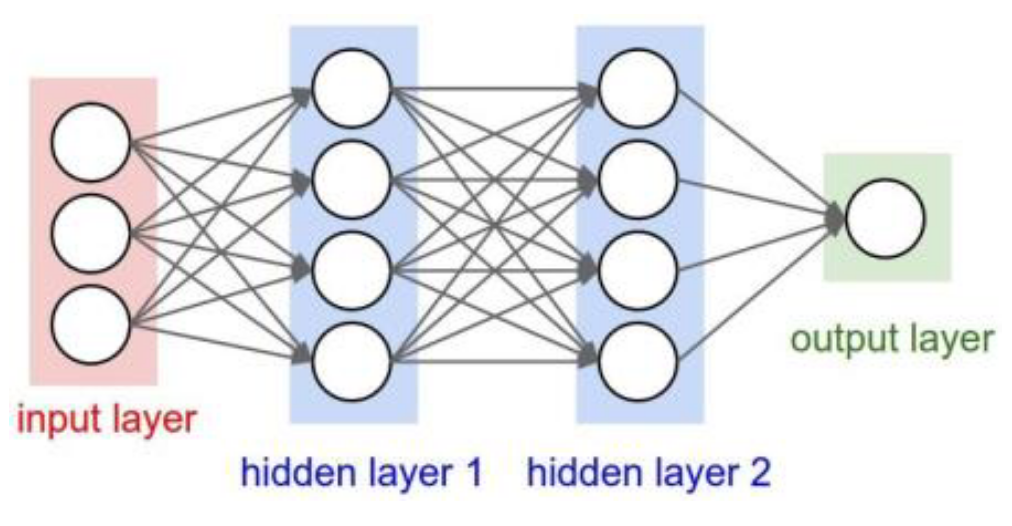
\includegraphics[width=0.75\columnwidth]{img/NN/NN1}
\end{center}
This is the scheme of a standard multi-layer feed-forward neural network (the standard before convolutional neural networks).\\

% End of L1, L2 is missing from the recordings, what to do?

\newpage

\subsection{Threshold Logic Unit}
The first \textbf{abstract model} for an artificial neuron of the brain. A \textbf{threshold logic unit} (TLU) is a processing unit (neuron) with several inputs. It can solve a very simple set of problems. \textbf{McCulloch-Pitts neuron}\\

There are several inputs reaching to the \textbf{core} (neuron), whose output is delivered to subsequent neurons which are connected with it.\\

A TLU is a processing unit in which the \textbf{output} is \textbf{governed} by a \textbf{threshold} $\theta$, if it has a \textbf{sufficient excitation} from the inputs, then the TLU becomes \textbf{active} (value 1) and generates the output $y$.

\begin{center}
	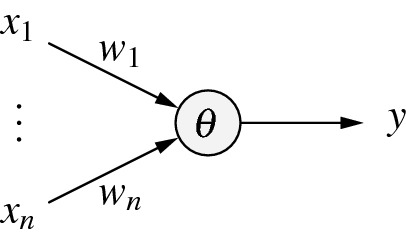
\includegraphics[width=0.35\columnwidth]{img/NN/TLU1}
\end{center}

There are $n$ inputs $x_1, \... \, , n_n$ and the TLU generates one output $y$. Each input is \textbf{weighted} ($w_1, \, ... \, , w_n$), some can be more relevant than others (we're considering data from the external world after all, not everything must be considered equally).\\

TLU conditions: 
$$
y = \begin{cases} 
	1 \;\; & \displaystyle \text{ if } \sum_{i=1}^n w_i x_i \geq \theta \\
	0 & \text{ otherwise }
\end{cases}
$$
The result is more dependent on the more important information. We can control how much of an influence each input has, determined by its weight $w$.\\ 

When the TLU is solicited enough if the \textbf{excitation} (weighted sum of the inputs) is \textbf{over the threshold} $\theta$ the output delivered to the terminal synapse and then to another neuron will be $1$, $0$ otherwise.\\

\newpage

\subsubsection{Conjunction Example}
The \textbf{result} is equal to \textbf{1 only when the two outputs are equal to 1}. There isn't a standard way to select the threshold $\theta$, it has to be chosen based on the function that has to be implemented. \\

In this case the $\theta$ chosen has to be greater than any individual weight.
$$ x_1 \wedge x_2 $$
\begin{center}
	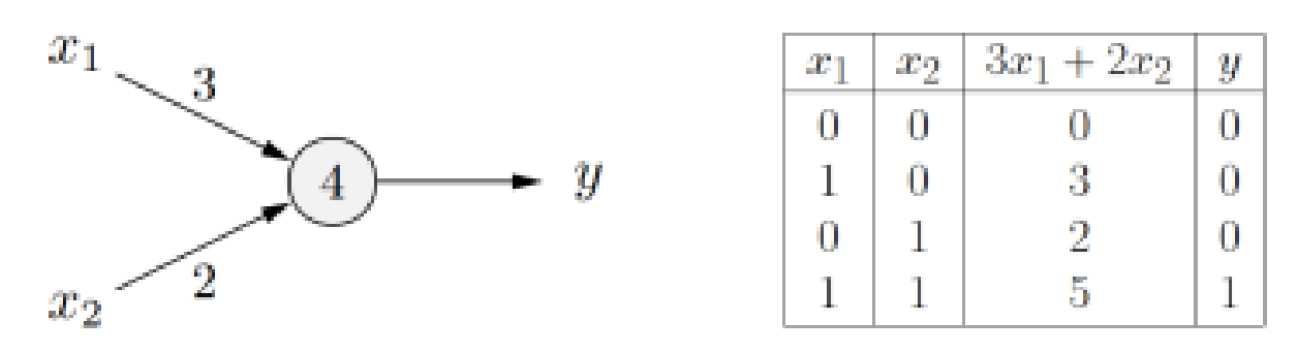
\includegraphics[width=0.85\columnwidth]{img/NN/TLU2}
\end{center}
(if I sum them, are they enough?).\\

In this example $w_1 \cdot x_1 + w_2 \cdot x_2 = 3 \cdot x_1 + 2 \cdot x_2$ has to be $\geq 4$ to have $y=1$.\\

\newpage

\subsubsection{Implication Example}
I can choose the value of the threshold in order to have the proper function, in this case applies on the same ways. How can I choose the interconnection weights? \\

The problem is that there are no general rules, I choose the weights according to the intrinsic relevance of each input variable.\\

How can I do that when we have a high number of inputs? We'll see that there is a procedure for doing that.
$$ x_2 \rightarrow x_1 $$
\begin{center}
	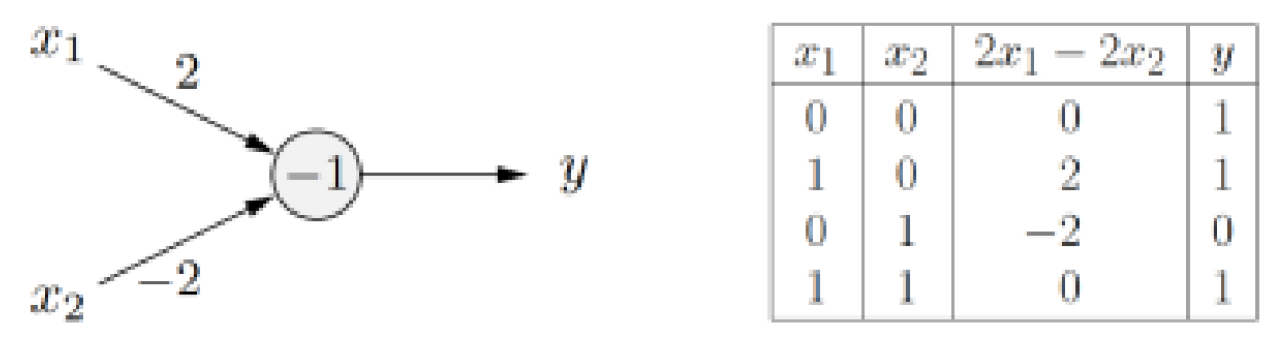
\includegraphics[width=0.85\columnwidth]{img/NN/TLU3}
\end{center}

This can also be expressed as $\neg x_2 \vee x_1$, so the output is true unless $x_2$ is true and $x_1$ is false.\\
The output "goes on" if the second one ($x_1$ in the example) is true without the first one ($x_2$ in the example) being true.\\
The weights must be tuned accordingly.\\

\newpage

\subsubsection{Multiple inputs example}
In this case we can see that we have three possible inputs, we can discriminate the inputs in excitatory input and inhibitory input. The first tries to contribute to the final computation of the neuron in such a way that the results will be greater than the threshold, the other neuron does the opposite.

\begin{center}
	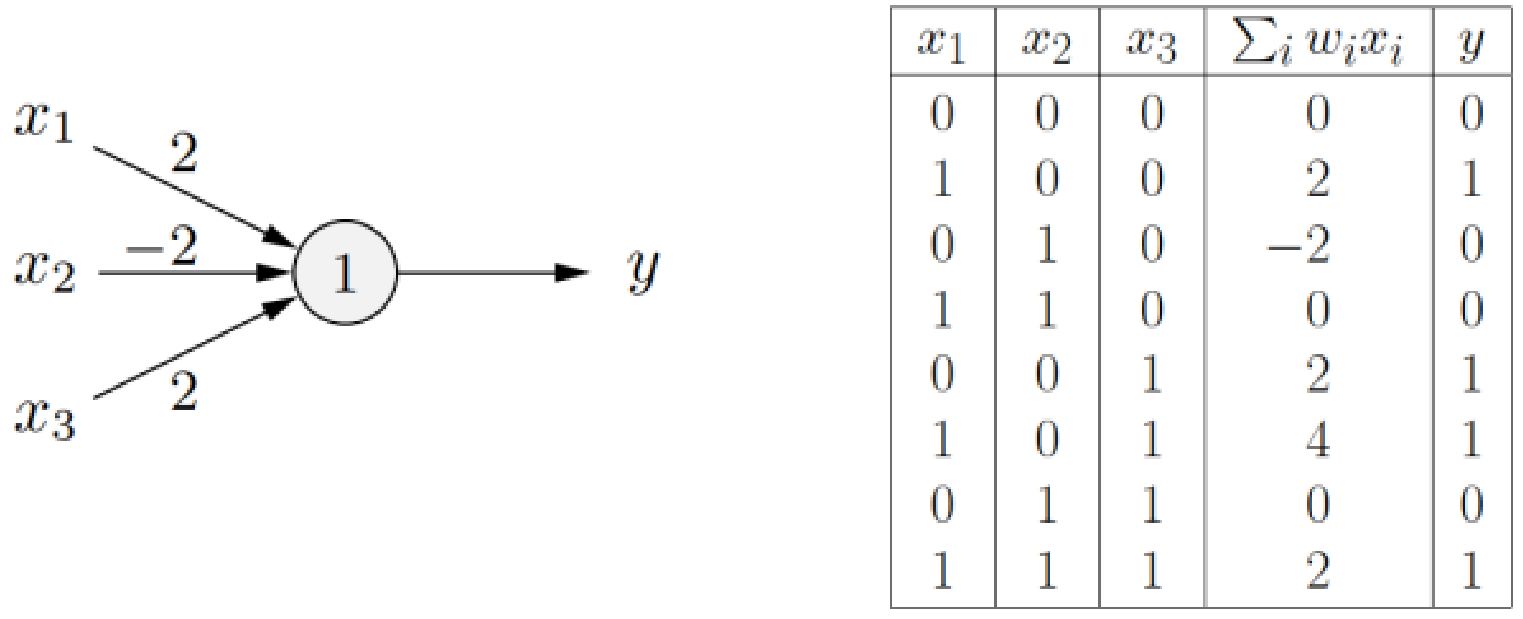
\includegraphics[width=0.85\columnwidth]{img/NN/TLU4}
\end{center}

The result is the weighted sum of multiple inputs, some of which "help" the output towards 1 while others "drag it" towards 0.\\

\newpage

\subsection{Geometric interpretation}
The geometric interpretation is significantly \textbf{helpful} to derive a method to \textbf{configure the threshold and the weights starting from the data}. \\

We will consider a single and simple TLU, we will try to understand how we can \textbf{interpret the behavior of the TLU} in a geometrical way. \\

It's possible to represent a straight line on a plane in any of the following forms:
\begin{itemize}
	\item {\makebox[4cm]{Explicit form: \hfill}} $g \equiv x_2 = b x_1 + c$
	
	\item {\makebox[4cm]{Implicit form: \hfill}} $g \equiv a_1 x_1 + a_2 x_2 + d = 0$
	
	\item {\makebox[4cm]{Point-Direction Form: \hfill}} $ g \equiv  \vec{x} = \vec{p} + k \vec{r} $
	
	\item {\makebox[4cm]{Normal Form: \hfill}} $ g \equiv  \left(\vec{x} - \vec{p}\right)^{\top} \vec{n} = 0 $
\end{itemize}

Any of these representations works to represent a straight line in the plane; we're considering just two variables $x_1$ and $x_2$.\\

The parameters are: 
\begin{itemize}
	\item {\makebox[1cm]{$b$: \hfill}} Gradient of the line
	\item {\makebox[1cm]{$c$: \hfill}} section of the $x_2$ axis (intercept)
	\item {\makebox[1cm]{$\vec{p}$: \hfill}} Vector of a point of the line (base vector)
	\item {\makebox[1cm]{$\vec{r}$: \hfill}} Direction vector of the line
	\item {\makebox[1cm]{$n$: \hfill}} Normal vector of the line
\end{itemize}

\begin{center}
	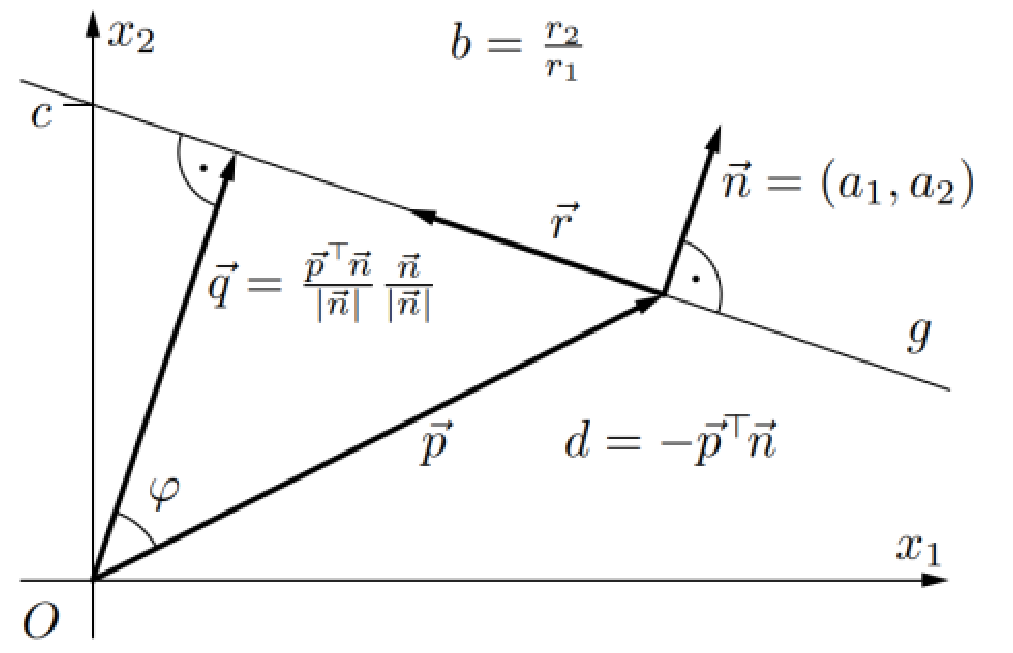
\includegraphics[width=0.5\columnwidth]{img/NN/GeomInt1}
\end{center}

In the case of the explicit/implicit form $b$ is the inclination (or gradient) of the line in respect to the horizontal axis, and $c$ is the interception with the vertical axis.\\

The normal $\vec{n}$ is the vector orthogonal to the straight line. The vector $\vec{p}$ identifies a point on the line. The distance from the line to the origin $O$ is given by $|\vec{q}|$.\\

\begin{center}
	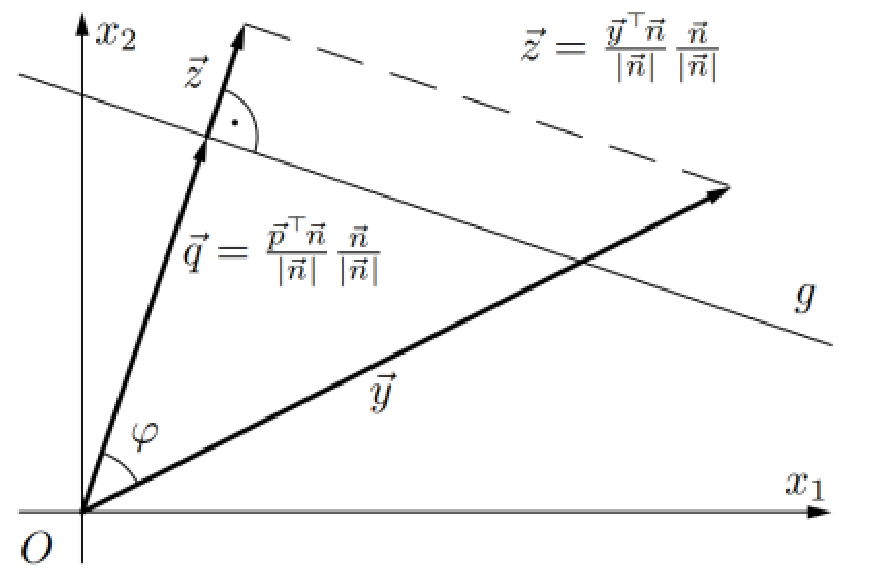
\includegraphics[width=0.65\columnwidth]{img/NN/GeomInt2}
\end{center}

We can \textbf{determine on which side of the line a point lands}, if we take the vector representing a point $\vec{y}$, and we compute the projection in the direction of the normal, the projection of this is 	the vector $\vec{z}$.\\

To understand on which side the points are, I just need to see if the vector $\vec{z}$ (which is the projection of our point) is shorter or longer than the point I observe on the straight line, which is pointed by $\vec{q}$. Basically, is the projection along the normal $\vec{n}$ shorter or longer (module is higher or lower) than our distance $\vec{q}$? \\

This means that all points (expressed by a vector) which have a module higher than the projected point onto the straight line ($\vec{q}$), are part of the plane above the straight line (they will satisfy the solution), vice versa, they will be below the plane if the module is shorter than $\vec{q}$ (they don't satisfy the condition).\\

Basically the \textbf{straight line} which \textbf{defines the behavior of our TLU}, splits the \textbf{plane in two parts} (since we're considering only $x_1$ and $x_2$).\\

\newpage

Solution for the conjunction and implication
\begin{center}
	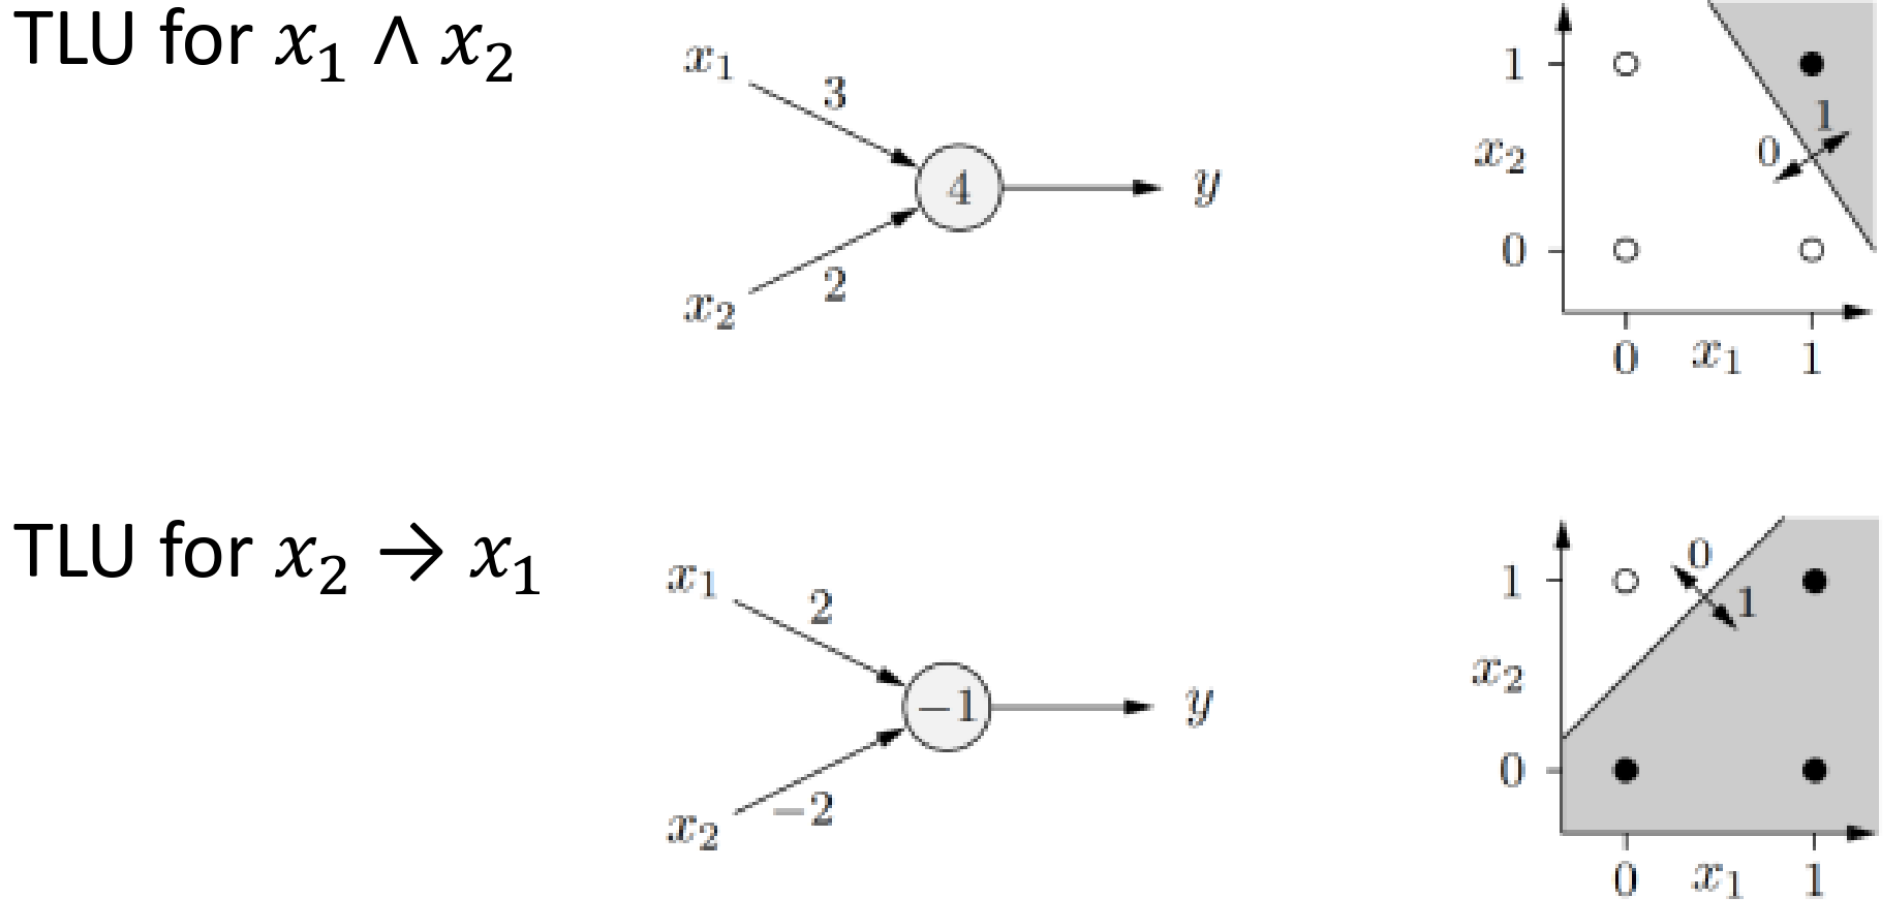
\includegraphics[width=0.95\columnwidth]{img/NN/TLU5}
\end{center}

Going back to our earlier examples, for the conjunction this means that there are 3 points in which the output will be 0 and 1 where the result is 1. The line can be represented as 
$$ 3 x_1 + 2 x_2 - 4 = 0 \Leftrightarrow x_2 = 2 - \frac{3}{2} x_1 $$

For the implication the output is 1 when the values are under the line, i.e. in 3 of the cases, under the line $2 x_1 - 2 x_2 + 1 = 0$.\\

For three variables the idea has to be generalized to a three-dimensional space, the line becomes a plane which divides the output values.
\begin{center}
	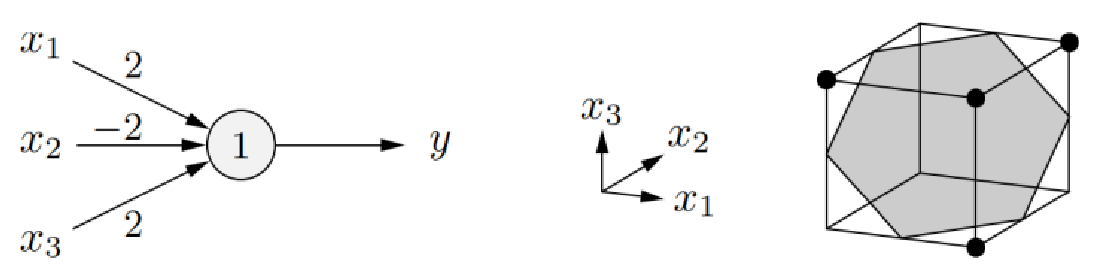
\includegraphics[width=0.85\columnwidth]{img/NN/TLU6}
\end{center}
Using our information the solution can be divided by this hexagon-looking plane (it's just "incomplete"), represented by the formula 
$$ 2x_1 -2x_2 +2x_3 -1 = 0 $$

\newpage

How are the \textbf{threshold and interconnection weights chosen}? We have to look at the geometrical distribution of the points for each possible output and have a line/plane that clearly separates each group.\\

If I can \textbf{clearly divide the groups I can use TLUs} to solve the problem.\\

For the bi-implication problem $x_1 \leftrightarrow x_2$
\begin{center}
	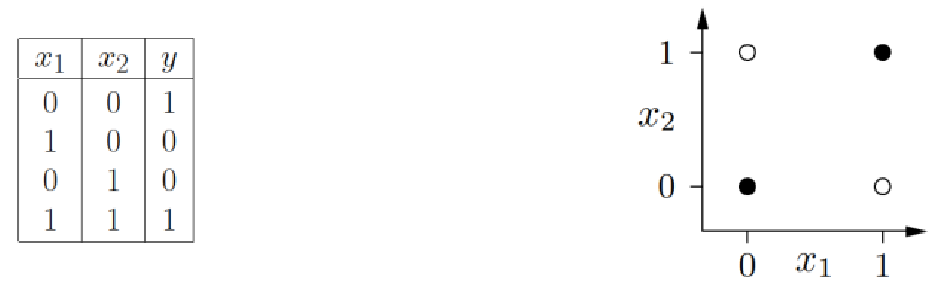
\includegraphics[width=0.9\columnwidth]{img/NN/TLU7}
\end{center}
There is no dividing line, the output groups cannot be separated with a straight line. As a consequence we can't have a TLU solving this problem.\\

\newpage

\subsubsection{Linear Separability}
\textbf{Two sets of points} in a \textbf{Euclidean space} are called \textbf{linearly separable}, if there exists at least one point, line, plane or hyperplane (depending on the dimension of the Euclidean space), such that \textbf{all points} of \textbf{one set} lie on \textbf{one side} and all points of the \textbf{other set} lie on the \textbf{other side} of this point, line, plane or hyperplane (or on it).\\

The point sets can be separated by a \textbf{linear decision function}.\\

This works in $n$ dimensions regardless; any TLU can have $n$ different inputs and each one will be represented by a dimension.\\

If I have a mono-dimensional space (a line) there will be a point dividing the 2 sets, if we look at a plane a line will divide the sets, for a three-dimensional space a plane divides the sets, ecc.\\

\subsubsection{Convex hull}
A set of points in a Euclidean space is called \textbf{convex} if it is non-empty and connected (that is, if it is a region) and for every pair of points in it every point on the straight-line segment connecting the points of the pair is also in the set.

In a Euclidean space a \textbf{convex set} is a set in which, for \textbf{each pair of points}, the \textbf{segment that connects them} is \textbf{entirely contained in the set}.\\

The \textbf{convex hull} of a set of points $X$ in a Euclidean space is the smallest convex set of points that contains $X$. Alternatively, the convex hull of a set of points $X$ is the intersection of all convex sets that contain $X$.\\

A \textbf{convex hull} is the smallest convex set of points that contains $X$.\\

\newpage

\subsection{Solution of the bi-implication problem}
Two sets of points in Euclidean Space are \textbf{linearly separable if and only if their convex hulls are disjoint} (have no point in common).\\

In the bi-implication problem, the convex hulls are the diagonal line segments. They share their intersection point and this means that they are not disjoint, therefore the double implication is not linearly separable.\\

We can try solving the complex problems a single neuron can't solve with more neurons
\begin{center}
	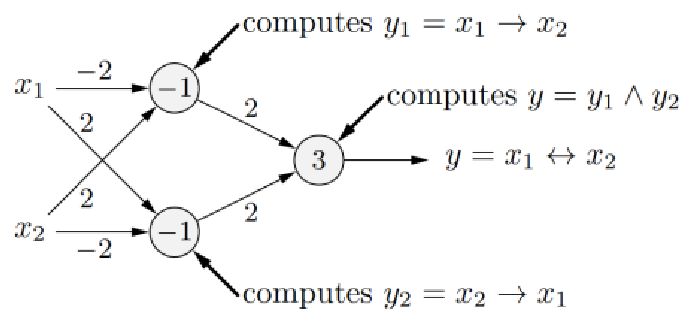
\includegraphics[width=0.7\columnwidth]{img/NN/TLU8}
\end{center}
We are creating a network of TLUs and splitting the problem into sub-problems.\\

The problem of implication can be solved in a single TLU and bi-implication is the intersection of implication from both ways so
$$ (x_1 \rightarrow x_2) \wedge (x_2 \rightarrow x_1) \implies x_1 \leftrightarrow x_2$$

\newpage

Let's see what happens geometrically
\begin{center}
	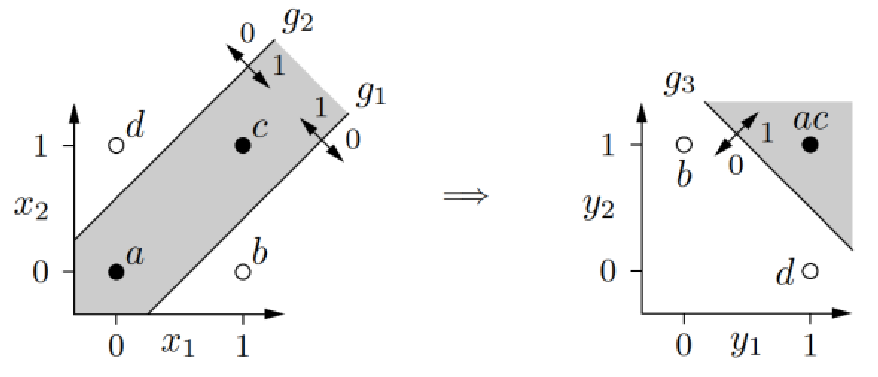
\includegraphics[width=0.85\columnwidth]{img/NN/TLU9}
\end{center}
The first graph represents the intersection between the first two TLUs, one outputs 1 for all values over the line $g_1$ (which represents $x_2 \rightarrow x_1$), while the other outputs 1 for all values under the line $g_2$ (which represents $x_1 \rightarrow x_2$).\\

We can then combine the outputs of the first TLUs $y_1$ and $y_2$ into the third (intersection), represented in the second graph. \\
This transforms the "stripe" from before into a plane, \textbf{identifying the linear separability}.\\

So we can see that with points $a$ and $c$ the final output is 1, while for $b$ and $d$ the solicitation is not enough.\\

\newpage

\subsection{Arbitrary boolean functions}
Following the previous reasoning, we can \textbf{work with any arbitrary boolean function} by having a \textbf{network of TLUs}.\\

For example, we have these values of $y$:
\begin{center}
	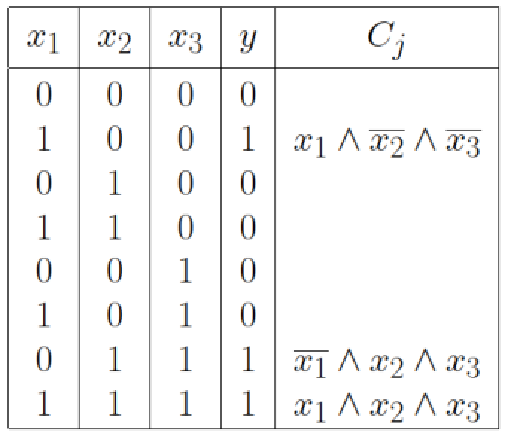
\includegraphics[width=0.35\columnwidth]{img/NN/ABF1}
\end{center}

We can now use a network to \textbf{compute each of the component for which the output has to be 1 and then put together} all possible values with a conjunction (OR on all values).\\

The resulting network is
\begin{center}
	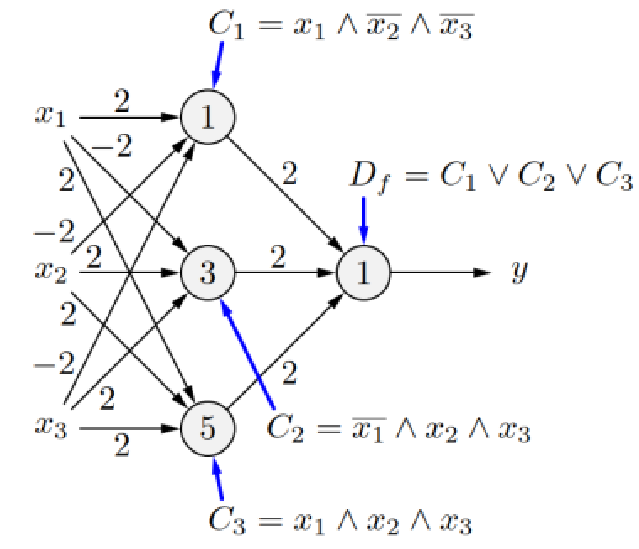
\includegraphics[width=0.6\columnwidth]{img/NN/ABF2}
\end{center}

% Should be end of L2, have no idea though, just guessin'

\newpage

\subsection{Training TLUs}
TLUs can solve linearly separated problems, but how can we get the right values for the parameters? We want to automatically understand these values.\\
The geometric interpretation can provide a way to construct TLUs but it has some problems
\begin{itemize}
	\item Not feasible for more than 3 inputs (we, sadly, live in a three-dimensional space)
	\item Not an automatic method, there's some human visualization needed to choose the values of the parameters and this process can't be mimicked directly by a machine
\end{itemize}

What we want to do is to have an automatic way which adjusts the weights and threshold of the network to reach the desired solution (if the two sets are linearly separable).\\

To have an \textbf{automatic training} we can start with \textbf{random values} for weights and threshold and determine the \textbf{error of the output} (how wrong the output is, based on the correct solution, which we know). We must define the \textbf{error} as a \textbf{function}, based on \textbf{weights and threshold} 
$$ e = e (w_1, \, ... \, , w_n , \theta) $$
We start with random values but we \textbf{adapt them} to make the \textbf{error smaller} and repeat this step until the error vanishes.\\

The basic concept is: get random values and change them step by step until they are correct, i.e. the error function is zero.\\

\newpage

\subsubsection{Negation example}
Considering a single input threshold logic unit for the negation $\neg x$
\begin{center}
	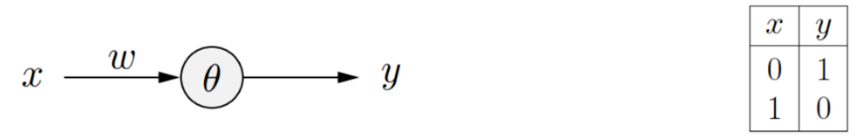
\includegraphics[width=0.85\columnwidth]{img/NN/TLU10}
\end{center}
We have one input, one weight, one threshold.\\

Output error as a function of weight and threshold
\begin{center}
	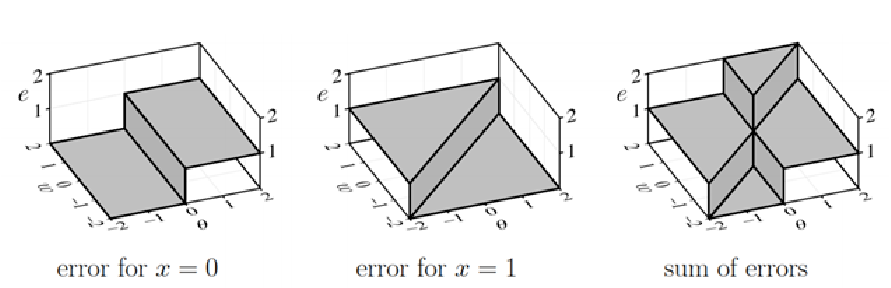
\includegraphics[width=0.85\columnwidth]{img/NN/error1}
\end{center}
This represents the error for all possible weights and threshold for each value of $x$.\\

By intersecting the graphs we can see the region for which the error function is zero for both values of $x$, and thus the wanted parameters. This is still a graphical way and not automated, it can't be directly mimicked by a machine.\\

To automate this we would need to read the shape of the error function in each point, since we need to know in which direction to go in order to obtain the correct result. With the error function as defined this is impossible since it consists of \textbf{plateaus} (all areas are flat). \\
If we're in a flat spot how can we determine which way to go if we want to go downwards? (we can't, it's not differentiable).\\

\newpage

We need to \textbf{modify the error function} to make it differentiable: if the computed output is wrong, take into account \textbf{how far from the weighted sum is from the threshold}. The error function tells us how wrong the result is, not only if it's right or wrong.\\

With the modified error function we obtain
\begin{center}
	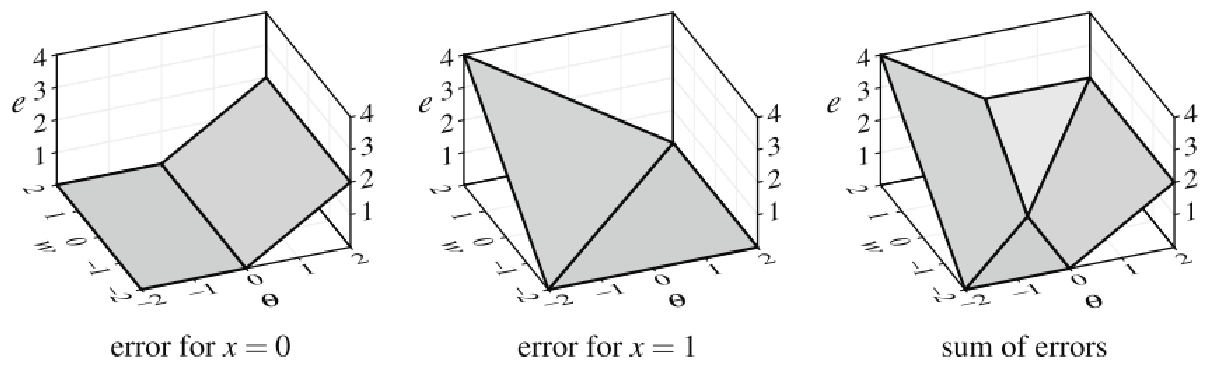
\includegraphics[width=0.85\columnwidth]{img/NN/error2}
\end{center}
Now if a TLU produces a wrong output we can adapt the weight and threshold in such a way to reduce the error, we want to \textbf{descend in the error landscape}. We simply \textbf{move in the direction in which the error function has the strongest downward slope}.\\

The parameter changes start with a random point in the error function and the values need to be iteratively adapted \textbf{according to the direction corresponding to the current point}. This means that if the output is 1 instead of 0 the threshold is too small and/or the weights are too large, hence they must be tuned accordingly (reducing the weights makes sense only if the corresponding input is 1). The contrary holds for the case in which the output is 0 when it should be 1.\\

This is a flattened version of the above image, where the dark parts represent values of error over zero; moving in the direction of the arrow decreases the error, until vanishing.
\begin{center}
	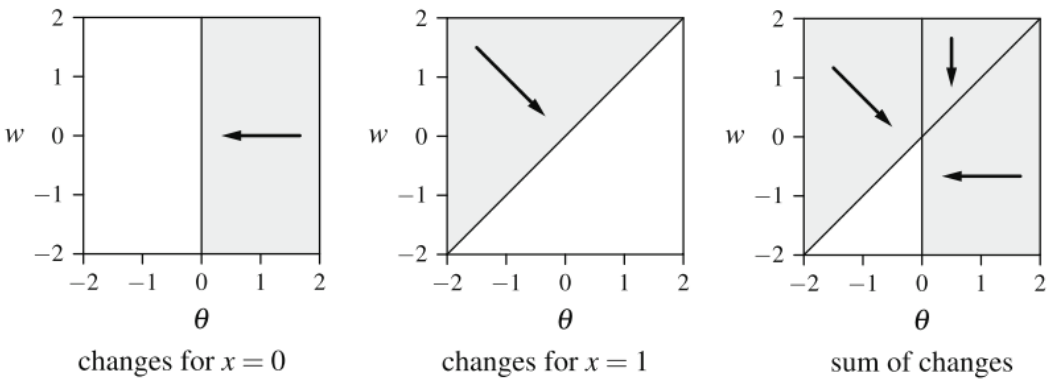
\includegraphics[width=0.8\columnwidth]{img/NN/error3}
\end{center}

\newpage

\subsubsection{Types of learning}
We can have two different types of training a neural network, differentiated by \textbf{how many learning patterns are applied at a time}; they are:
\begin{itemize}
	\item \textbf{Online learning:} we consider one learning pattern at a time, and change the weight accordingly. In the earlier example we may consider the input $x=0$, adapt the weights accordingly, do the same for $x=1$ and repeat until the error vanishes. With every example available a training step is carried out.\\
	
	\item \textbf{Batch learning:} we collect a sequence of learning patterns during a learning epoch and then compute the cumulative parameter corrections to be applied for the entire set of learning patterns. After all the examples have been explored the aggregated changes are applied. This is also repeated until the error vanishes.\\
\end{itemize}

Basically the difference is that in the online learning we give one example at a time (with the relative adaptations), while batch learning applies the changes only after a number of examples.\\

Batch learning can avoid wasting resources with parallel processing of the examples, if all the samples in the dataset are already known. \\

If we want something that adapts while new data is acquired online learning might be better.\\

\newpage

\subsubsection{Delta Rule (Widrow-Hoff)}
It's a \textbf{training rule}, how do we determine the adaptation of the weights to minimize errors?\\

Given
\begin{itemize}
	\item $\vec{x} = \left(x_1, \, ... \, , x_n \right)^T$ as an \textbf{input vector} of a TLU
	\item $o$ as the \textbf{desired output} of the vector
	\item $y$ as the \textbf{actual output} of the TLU
\end{itemize}

We have an output $y$ and a desired value $o$ and the \textbf{difference between them tells us how to adapt the values}.\\

If $y \neq o$, then the threshold $\theta$ and the weight vector $\vec{w} = \left(w_1, \, ... \, , w_n\right)^T$ are \textbf{adapted as follows} to \textbf{reduce the error}: 

$$ \theta^{(new)} = \theta^{(old)} + \Delta \theta, \text{ with } \Delta \theta = - \eta (o - y) $$
$$ w_i^{(new)} = w_i^{(old)} + \Delta w_i, \text{ with } \Delta w_i = \eta (o - y) x_i $$ 
$$\forall i \in \left\{1, \, ... \, , n\right\}$$

Where $\eta$ is the \textbf{learning rate}, i.e. how much do we value new inputs, it determines the "speed" and size of the updates, 1 at the most, usually small in the range of $2^{-4}$ to avoid excessive oscillation. \\

It's basically old value $+$ delta multiplied by a factor $\eta$ (and the input for the weights).\\

\newpage

Example for online training with starting $\theta = 1.5$, $w = 2$ and $\eta = 1$
\begin{center}
	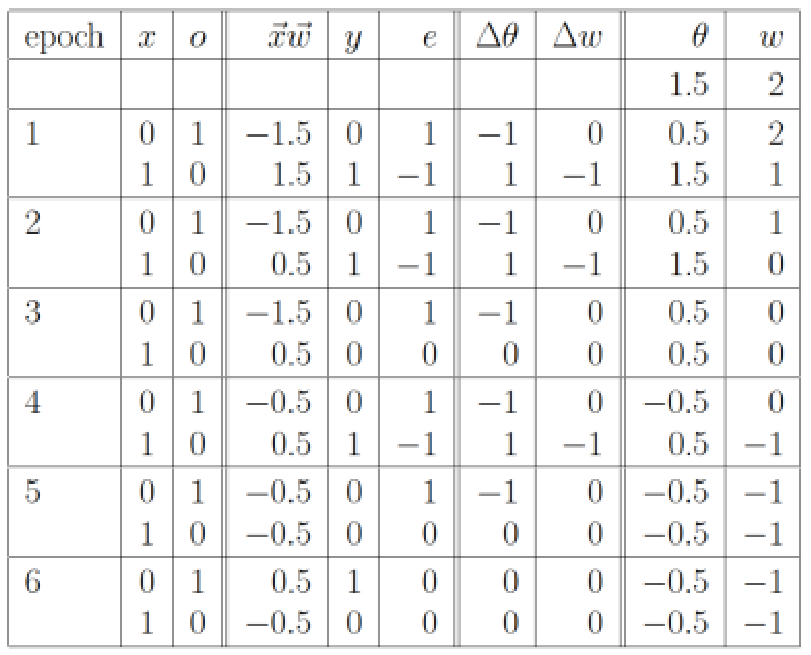
\includegraphics[width=0.6\columnwidth]{img/NN/delta1}
\end{center}

Example for batch training with the same starting values
\begin{center}
	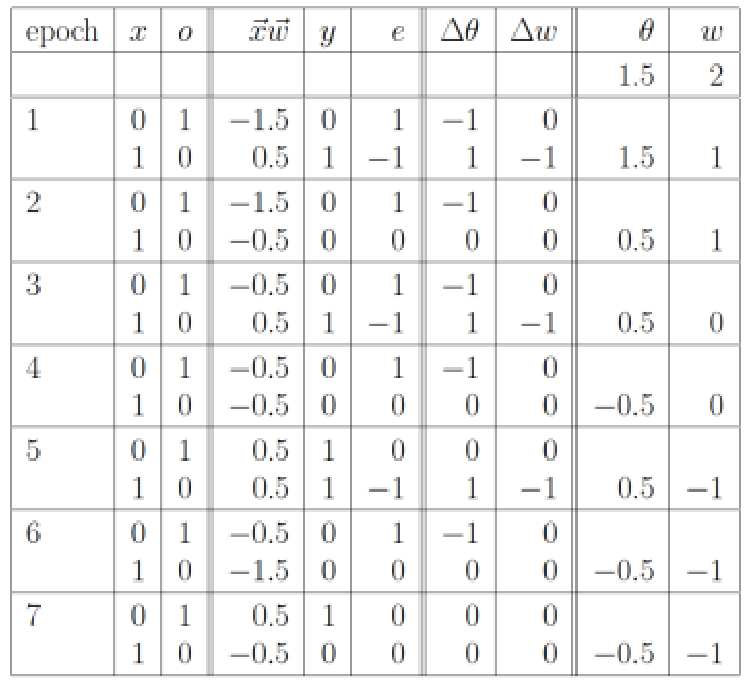
\includegraphics[width=0.6\columnwidth]{img/NN/delta2}
\end{center}
The change is delayed, so it takes one epoch more.\\

We can unify the adaptation rule by turning $\theta$ into a weight: fix $\theta = 0$ and add an imaginary input fixed at $x_0 = 1$, this input can be weighted with the negated threshold.\\

\newpage

The different progression of online and batch training and a geometric interpretation
\begin{center}
	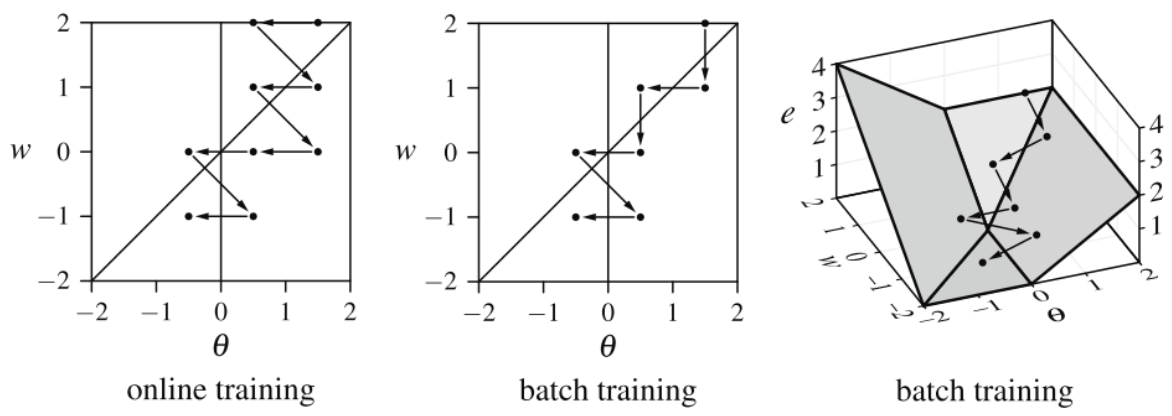
\includegraphics[width=0.9\columnwidth]{img/NN/delta3}
\end{center}
We can see that we're descending from a high value of the error function (the starting random value) to a smaller one each time.\\

\newpage

\subsubsection{Convergence Theorem}
Convergence: at some point the error will become 0.\\

Let $L = \left\{ (\vec{x}_1, o_1), \, ... \, , (\vec{x}_m, o_m)\right\}$ be a \textbf{set of training patterns}, each \textbf{consisting} of an \textbf{input vector} $x_i \in \mathbb{R}^n$ (there can be $n$ inputs) and a \textbf{desired output} $o_i \in \{0, 1\}$ (out can go one of the two values).\\

Furthermore, let $L_0 = \left\{\left(\vec{x}, o\right) \in L | o = 0 \right\}$ and $L_1 = \left\{ \left(\vec{x}, o\right) \in L | o = 1\right\}$ (respectively, all the training patterns for which the output should be 0 and all patterns for which it should be 1, you need both to describe all cases).\\

If $L_0$ and $L_1$ are \textbf{linearly separable} (all zeros on one side of a line, all the ones on the other), that is, if $\vec{w} \in \mathbb{R}^n$ and $\theta \in \mathbb{R}$ exist such that
$$ \forall \left(\vec{x}, 0 \right) \in L_0: \, \vec{w}^T \vec{x} < \theta \;\; \text{ and}$$
$$ \forall \left(\vec{x}, 1 \right) \in L_0: \, \vec{w}^T \vec{x} \geq \theta $$

then \textbf{online as well as batch training terminate}. If the outputs are linearly separable we have convergence.\\

The algorithm \textbf{terminates only when the error vanishes}. The resulting weights and threshold solve the problem.\\

For \textbf{non-linearly separated} problems, the \textbf{algorithm doesn't terminate}. It oscillates and repeats computation for the same non-solving $\vec{w}$ and $\theta$.\\

\newpage

\subsubsection{Encoding Problems}
The \textbf{parameter correction depends on the encoding of Boolean values}. We use $false = 0$ and $true = 1$ and this may result in less opportunities for correcting the parameters by means of the Delta rule. We cannot adapt a 0, and it's a numerical problem, we can't change the weight corresponding to an input of $false$ since the formula for the weight change contains the input as a factor (anything $\cdot 0 = 0$).\\

To speed up learning and having more frequent correction opportunities we can adapt a different encoding scheme: \textbf{ADALINE} (\textbf{ADA}ptive \textbf{LIN}ear \textbf{E}lement).\\

\textbf{ADALINE} relies on the \textbf{encoding} $true = +1$ \textbf{and} $false = -1$.\\

Basically, in the case of $false$ we don't do anything and we want to do something; we do that by changing the $false$ weight to $-1$.\\

% End of NN L3 (Che fatica diocane)

\newpage

\subsection{Artificial Neural Network}
An Artificial Neural Network (ANN) has a simple \textbf{general definition}: it's a \textbf{directed graph} $G= (U,C)$ whose \textbf{vertices} $u \in U$ are called \textbf{neurons} or units and whose \textbf{edges} $c \in C$ are called \textbf{connections}.\\

The set of \textbf{vertices} (neurons) is \textbf{partitioned into}: 
\begin{itemize}
	\item Set $U_{in}$ of \textbf{input} neurons (receive input from the environment).\\
	
	\item Set $U_{out}$ of \textbf{output} neurons (emit output to the environment).\\
	
	\item Set $U_{hidden}$ of \textbf{hidden} neurons (have no contact with the environment).\\
	
\end{itemize}
The sets $U_{in}$ and $U_{out}$ don't need to be disjoint; a neuron can be both input and output.\\



\subsubsection{General structure of a neuron}
Each \textbf{connection} (arc from a neuron to the other) $(v,u) \in C$ \textbf{possesses a weight} $w_{uv}$.\\

Here we can see an example of structure of a neuron:
\begin{center}
	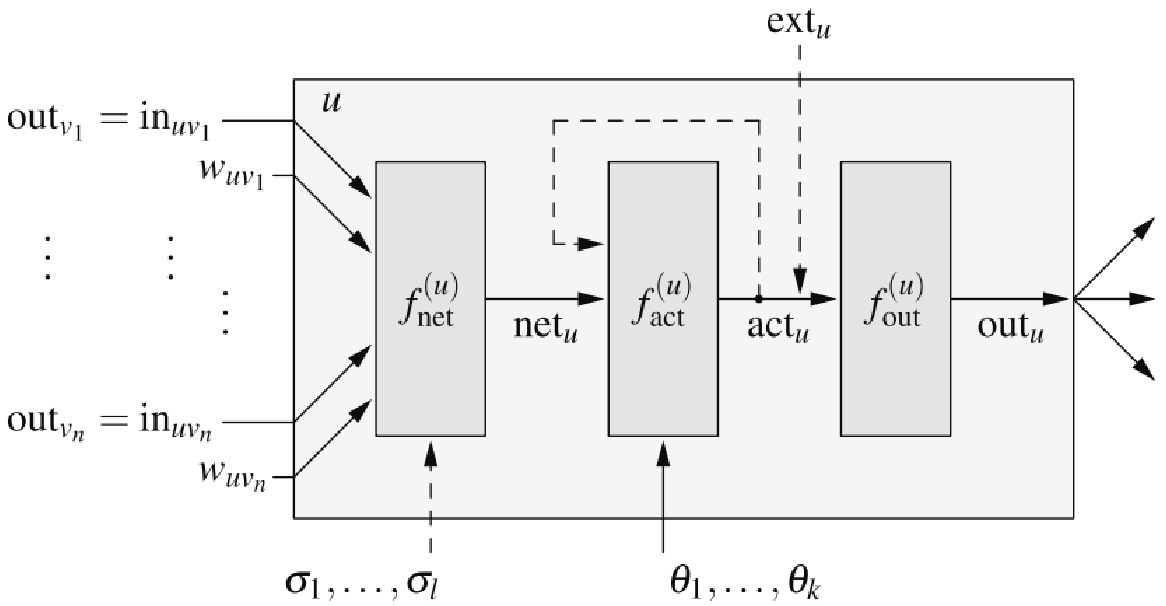
\includegraphics[width=0.9\columnwidth]{img/NN/neuron1}
\end{center}

\newpage

We can see that there are inputs coming in the network, which represent the stimulus that the neuron receives from the external world, here called $in_{uv_n}$, each of them with the associated weight $w_{uv_n}$.\\

Each input signal can be the output of a previous neuron, the output $out_{v_n}$ for neuron $v_n$ becomes $in_{uv_n}$.\\

The \textbf{inputs} are \textbf{processed in three stages}: 
\begin{itemize}
	\item \textbf{Input function} $f^{(u)}_{net}$: from inputs to $net_u$, takes all the \textbf{inputs} and \textbf{combines them} according to their value and relative relevance (weight), to \textbf{generate the global solicitation} of the neuron.\\
	
	\item \textbf{Activation function} $f^{(u)}_{act}$: \textbf{analyzes} the global \textbf{input} and \textbf{generates the activation status} of the neuron. It tells us if the neuron is sufficiently excited. Usually non-linear, the non-linearity gives the neuron its processing capability.\\
	
	\item \textbf{Output function} $f^{(u)}_{net}$: takes the excitation status of the neuron and \textbf{elaborates the final status} to deliver to subsequent neurons.\\
	
\end{itemize}

Each \textbf{neuron} $u \in U$ possesses three (real-valued) \textbf{state variables}:
\begin{itemize}
	\item the \textbf{neuron input} $net_u$: value going in the neuron, usually the sum of all weighted inputs 
	\item the \textbf{activation} $act_u$: the result of the neuron applying a transformation on the input
	\item the \textbf{output} $out_u$: the final output, after processing the result of the activation
\end{itemize}
There's also a fourth state variable: 
\begin{itemize}
	\item the \textbf{external input} $ext_u$: it lets us add another variable after the activation phase, if needed
\end{itemize}

\newpage

\subsection{Types of Artificial Neural Network}
There are \textbf{two types of ANN}: 
\begin{itemize}
	\item \textbf{Feed-forward network (FNN):} its graph doesn't contain any cycle.\\
	
	\item \textbf{Recurrent network (RNN):} the graph contains cycles (backwards connections).\\
\end{itemize}

The \textbf{operation of an ANN} can be divided in: 
\begin{enumerate}
	\item \textbf{Input phase:} external \textbf{inputs} are \textbf{acquired} by input neurons. Inputs are fed into the network\\
	
	\item \textbf{Work phase:} external inputs are switched off while \textbf{new outputs are computed} by each neuron. It's the phase in which the output of the network is computed.\\
\end{enumerate}

If a neuron does not receive any network input, because it doesn't have any predecessor, it simply maintains its activation (and thus its output).\\

During the working phase, if the input values are steady the computation doesn't change (as in the FNN). \\
That is not always the case, for example in a RNN the cycles could modify the input of another neuron which has already finished computation, possibly changing its output status.\\

\textbf{Re-computation} of a neuron output occurs if any of its input change. Temporal order of re-computation depends on the type of ANN.\\
This phase continues until the eternal \textbf{output are steady}, or a \textbf{maximum number of} re-computation \textbf{iterations} is reached.\\

All neurons of a network may \textbf{recompute} their outputs at the \textbf{same time} (\textbf{synchronous update}) drawing on the old outputs of their predecessor, or we can also \textbf{define an order} in which the neurons \textbf{compute their new output} one after the other (\textbf{asynchronous update}).\\

\newpage

\subsubsection{Feed Forward Neural Network}
\begin{enumerate}
	\item \textbf{Computation} proceeds \textbf{from input} neurons progressively \textbf{toward output neurons} by following the topological order of the neuron (left to right basically) in the network.\\
	
	\item The \textbf{external inputs are frozen}.\\
	
	\item \textbf{Input neurons compute their outputs} which are maintained steady and \textbf{forwarded} to the connected neurons.\\
	
	\item \textbf{Neurons connected} to preceding neurons with steady outputs \textbf{generate their respective outputs} and \textbf{propagate them} forward to the subsequent neurons, \textbf{until the external outputs are generated}. \\
\end{enumerate}

\newpage

\subsubsection{Recurrent Neural Network}
Example of a simple recurrent neural network
\begin{center}
	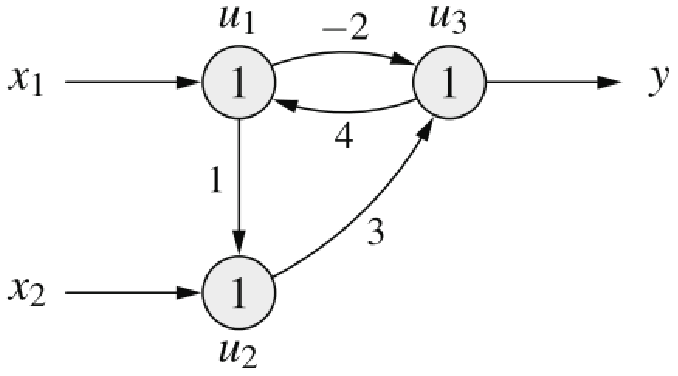
\includegraphics[width=0.45\columnwidth]{img/NN/RNN1}
	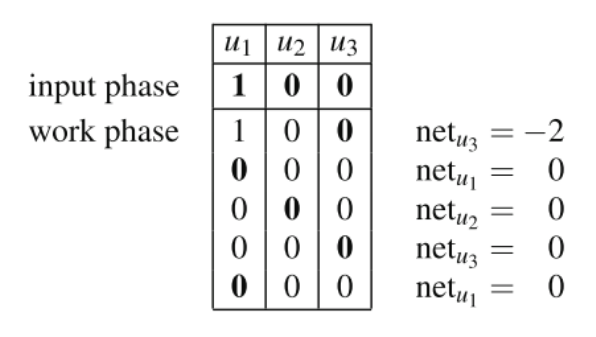
\includegraphics[width=0.45\columnwidth]{img/NN/RNN2}
\end{center}
The order in which the neurons are updated is $u_3$, $u_1$, $u_2$. On the right the dataset assumes this ordering with inputs $x_1 = 1$ and $x_2 = 0$. The updates of the neurons are represented in bold. \\

The phases are: 
\begin{itemize}
	\item \textbf{Input phase:} initial activation/outputs. In the input phase the values of $u_1$ and $u_2$ are determined by the external inputs, while $u_3$ is initialized to the (arbitrarily chosen) value 0.
	\item \textbf{Work phase:} activation/outputs of the next neuron to update are computed from the previous outputs and the weights/threshold. Note that external outputs are no longer available as they have been switched off.
	\item \textbf{Stable state:} a unique output is reached.
\end{itemize}

If we change the order of the updates to $u_3$, $u_2$, $u_1$
\begin{center}
	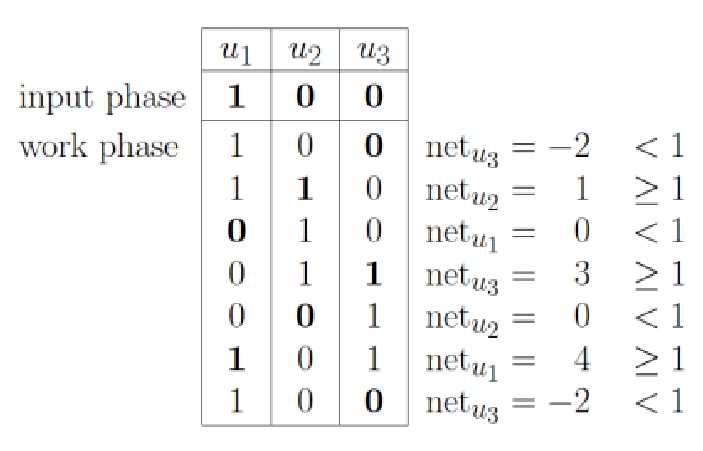
\includegraphics[width=0.45\columnwidth]{img/NN/RNN3}
\end{center}
The behavior changes completely. As the steps proceed it becomes clear that the seventh step is identical to the first and the computation will repeat indefinitely. The output of the NN depends on the step after which the work phase is terminated. \textbf{No stable state}, oscillation of output.\\

\newpage

\subsection{Configuration of a Neural Network}
The structure of the network can be divided in two categories, based on the learning procedure (how the data is given):
\begin{itemize}
	\item \textbf{Fixed learning task} (supervised learning)\\
	\item \textbf{Free learning task} (unsupervised learning)\\
\end{itemize}

Training a neural network consists in adapting the connection weights and possibly some other parameter (like thresholds) such that a certain criterion is optimized.\\

\newpage

\subsubsection{Fixed learning task}
A \textbf{fixed learning task} $L_{fixed}$ for a neural network with
\begin{itemize}
	\item $n$ \textbf{input neurons} $U_{in} = \left\{u_1, \, ... \, , u_n \right\}$
	\item $m$ \textbf{output neurons} $U_{out} = \left\{v_1, \, ... \, , v_m \right\}$
\end{itemize}
is a \textbf{set of training patterns} $l = \left(\vec{i}^{(l)}, \vec{o}^{(l)}\right)$ each consisting of 
\begin{itemize}
	\item an \textbf{input vector }$\vec{i}^{(l)} = \left(ext_{u_1}^{(l)}, \, ... \, , ext_{u_n}^{(l)}\right)$
	\item an \textbf{output vector} $\vec{o}^{(l)} = \left(o_{v_1}^{(l)}, \, ... \, , o_{v_m}^{(l)}\right)$
\end{itemize}

This is also called \textbf{supervised learning}.\\
It basically consists in giving the NN the inputs and their relative outputs from which to learn. We give the output vector which the network should be able to generate at the end of the configuration.\\

A fixed learning task is solved when for all training patterns $l \in L_{fixed}$ the neural network computes, from the external inputs contained in the input vector $\vec{i}^{(l)}$ of a training pattern $l$, the outputs contained in the corresponding output vector $\vec{o}^{(l)}$. Basically it's solved if it gives the right answer for all training inputs we give it.

\paragraph{Error of a fixed learning task:} how well a neural network solves a given fixed learning task. Essentially it's the \textbf{difference between desired and actual outputs}

$$ e = \sum_{l \in L_{fixed}} e^{(l)} ) = \sum_{v \in U_{out}} e_v = \sum_{l \in L_{fixed}} \sum_{v \in U_{out}} e_v^{(l)} $$
$$ \text{where } \;\; e_v^{(l)} = \left(o_v^{(l)} - out_v^{(l)}\right)^2 $$

To get a number that reflects the final quality of the network we consider the difference between the actual and desired output. The square is there to avoid negative signs; it also weighs more severely large deviations from the desired output (mean square error).\\
Basically, the error is the sum of all output discrepancies across all instances.\\
In practice, the optimum can rarely be achieved and thus one may have to accept a partial or approximate solution.

\newpage

\subsubsection{Free learning task}
A \textbf{free learning task} $L_{free}$ for a neural network with: 
\begin{itemize}
	\item $n$ \textbf{input neurons} $U_{in} = \left\{u_1, \, ... \, , u_n\right\}$ 
\end{itemize}
is a \textbf{set of training patterns} $l = \left(\vec{i}^{(l)}\right)$ each consisting of
\begin{itemize}
	\item an \textbf{input vector} $\vec{i}^{(l)} = \left(ext_{u_1}^{(l)}, \, ... \, , ext_{u_n}^{(l)}\right)$
\end{itemize}

There is no output vector. It's also called \textbf{unsupervised learning}.\\
The desired behavior is not defined a priori, it's up to the learning algorithm to produce an output vector.\\

There is \textbf{no desired output} for the training patters. Outputs can be chosen freely by the training method.\\

\textbf{Solution}: \textbf{similar inputs} should lead to \textbf{similar outputs}, the learning should lead to the \textbf{clustering} of similar input vectors so that the same output is produced for all vectors in the same cluster.\\

An important aspect for this type of training is \textbf{how the similarity} between patterns \textbf{is measured}, for example, with the help of a \textbf{distance function}. \\

\paragraph{Preprocessing:} to give all neurons the same importance we need to pre-process the data. For each component of the input vector we need to compress the representation in the same range, we need to \textbf{normalize the input vector} (e.g. z-score normalization)
$$ \mu_k = \frac{1}{|L|} \sum_{l \in L} ext_{u_k}^{(l)}$$
we also need to be sure that the standard deviation $\sigma_k$ is adjusted as well
$$ \sigma_k = \sqrt{\frac{1}{|L| - 1} \sum_{l \in L} \left(ext_{u_k}^{(l)} - \mu_k \right)^2}$$

This is the standard normalization of the deviation $\sigma_k$, there's another possibility which is called \textbf{unbiased standard deviation} (often preferred by statistician since is not polarized on the two direction).\\

The normalization can be necessary to avoid certain numerical problems which can result from an unequal scaling of the different input variables.\\

All the stimuli are recomputed with respect to the average value and they are normalized in dimension dividing them by the standard deviation. The input vector is normalized to expected value (arithmetic mean) equal to 0 and the standard deviation equal to 1
$$ ext_{u_k}^{(l)(new)} = \frac{ext_{u_k}^{(l)(old)} - \mu_k}{\sigma_k} $$
Subtract the mean and divide by 1, all features get kinda in the range from -1 to 1.\\

\paragraph{Data representation:} we need to represent different type of data: 
\begin{itemize}
	\item Numeric data: 
	\begin{itemize}
		\item Real numbers 
		\item Integer numbers
	\end{itemize}
	\nn
	
	\item Non-numeric (symbolic) data: 
	\begin{itemize}
		\item Symbols, 1-in-N encoding
	\end{itemize}
\end{itemize}

Simply numbering the different values of attributes can lead to undesired effects if said numbers don't reflect a natural order of the values, so a better option is \textbf{1-in-N encoding} in which each nominal attribute is assigned as many (input or output) neurons as it has values: each neuron corresponds to one attribute value.\\

With the input of a training pattern, the neuron that corresponds to the value of the nominal attribute is set to 1, while all others are set to 0. Only 1 in $n$ neurons (where $n$ is the number of attributes values) is set to 1, the others to 0 (explains the name).\\
Basically a string of $n$ bits in which only the bit that represent our symbol is raised.\\

% End of NN L4 (sempre una fatica diocane), Pag 35

\newpage

\subsection{Multi-layer Perceptrons MLP}
An \textbf{$r$-layered perceptron} is a feed-forward neural network with a \textbf{strictly layered structure}.\\

Each layer receives inputs only from the previous one (or the external world) and delivers its output to the subsequent layer; jumps are not allowed. Connections exist only between neurons of consecutive layers. Usually a neuron is fully connected to the neurons of its adjacent layers.\\

It's a common structure and can have significant processing capabilities, since you can increase them by simply adding more neurons/layers.\\

There are different kinds of layers:
\begin{itemize}
	\item \textbf{input} layers
	\item \textbf{hidden} layers
	\item \textbf{output} layers
\end{itemize}

\textbf{General structure} for an $r$-layered perceptron:
\begin{center}
	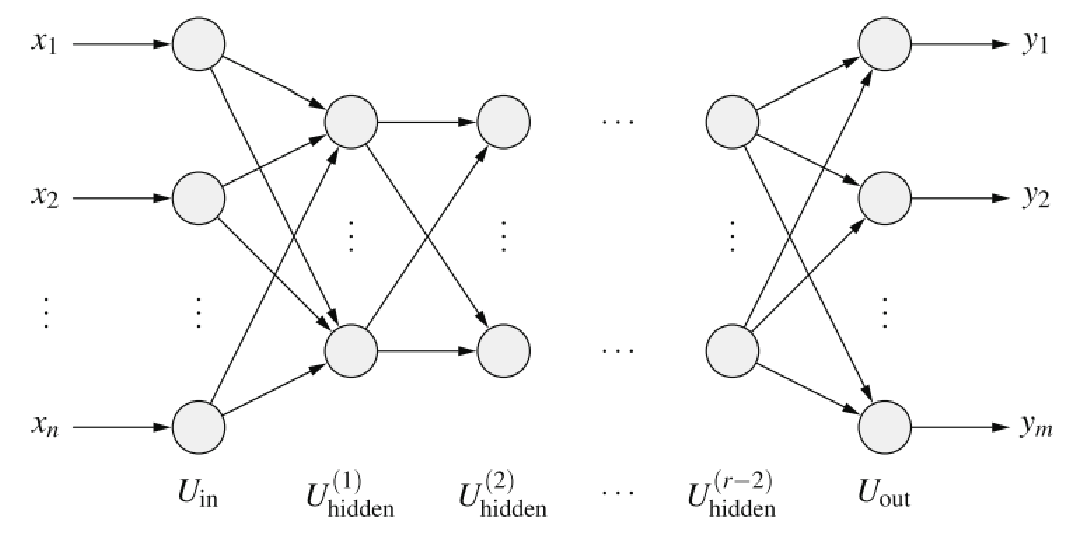
\includegraphics[width=0.9\columnwidth]{img/NN/MLP1}
\end{center}

\newpage

The \textbf{network input function} of each hidden neuron and of each output neuron is the \textbf{weighted sum of its inputs}
$$ f_{net}^{(u)} \left(\vec{w}_u, \vec{in}_u\right) = \vec{w}_u^T \vec{in}_u = \sum_{v \in pred(u)} w_{uv} out_v $$
Basically just each input times their weight, for each neuron.\\

%\newpage

The \textbf{activation function} of each \textbf{hidden neuron} is a so-called \textbf{sigmoid function}, a monotonically non-decreasing function; non-linear (to add complexity), usually with bounded output (e.g. from -1 to 1), continuous and differentiable
$$ f: \, \mathbb{R} \rightarrow [-1, 1] \text{ with } \lim_{x \rightarrow - \infty} f(x) = -1 \text{ and } \lim_{x \rightarrow \infty} f(x) = 1 $$
(if the bounds are $[-1, 1]$).\\

Depending on what we want to achieve, the \textbf{activation function} of each \textbf{output neuron} can also be a \textbf{sigmoid or} a \textbf{linear} function; basically the output neurons can take all the inputs and throw them outside (linearly), they don't elaborate further.\\

Some examples of sigmoid activation functions:
\begin{itemize}
	\item Step function (left):
	$$ f_{act} (net, \theta) = \begin{cases}
		1, \;\; & \text{ if } net \geq \theta \\
		0, & \text{ otherwise}
	\end{cases} $$
	\item Semi-linear function (right):
	$$ f_{act} (net, \theta) = \begin{cases}
		1, \;\; & \text{ if } net > \theta + \frac{1}{2} \\
		0, & \text{ if } net < \theta - \frac{1}{2} \\
		(net - \theta) + \frac{1}{2} & \text{ otherwise}
	\end{cases} $$
\end{itemize}
\begin{center}
	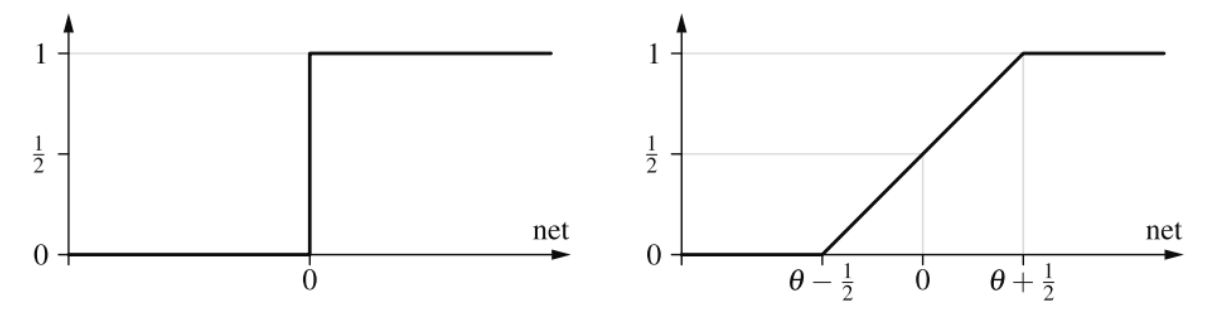
\includegraphics[width=0.9\columnwidth]{img/NN/sigmoid1}
\end{center}

\newpage

\begin{itemize}
	\item Sine until saturation (left):
	$$ f_{act} (net, \theta) = \begin{cases}
		1, \;\; & \text{ if } net > \theta + \frac{\pi}{2} \\
		0, & \text{ if } net < \theta - \frac{\pi}{2} \\
		\frac{\sin(net - \theta) + 1}{2} & \text{ otherwise } 
	\end{cases} $$
	\item Logistic function (right):
	$$ f_{act} (net, \theta) = \frac{1}{1 + e^{-(net - \theta)}} $$
\end{itemize}
\begin{center}
	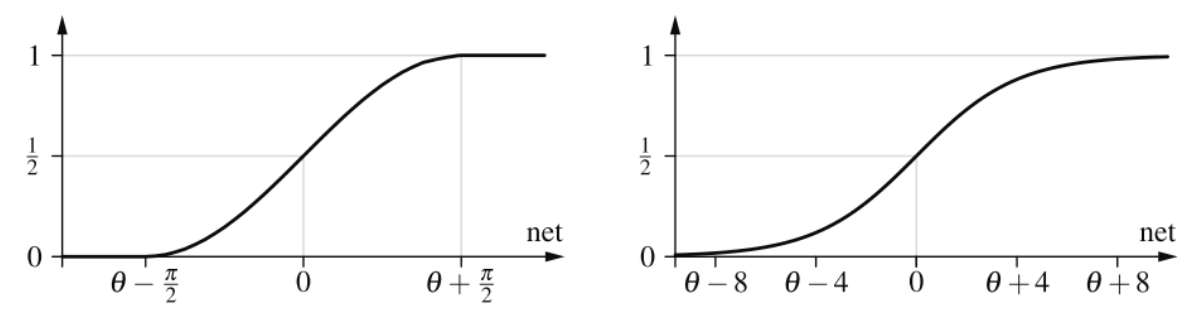
\includegraphics[width=0.9\columnwidth]{img/NN/sigmoid2}
\end{center}
These are some \textbf{unipolar} sigmoid activation functions.\\

Sometimes \textbf{bipolar sigmoid functions} are used (ranging from $-1$ to $+1$, two poles, not only one), like the \textbf{hyperbolic tangent}, this allows a better response to stimuli, in contrast to something like the step function which can only be 0 or 1
$$ f_{act} (net, \theta) = \tanh (net - \theta) = \frac{2}{1 + e^{-2(net-\theta)}} - 1 $$
\begin{center}
	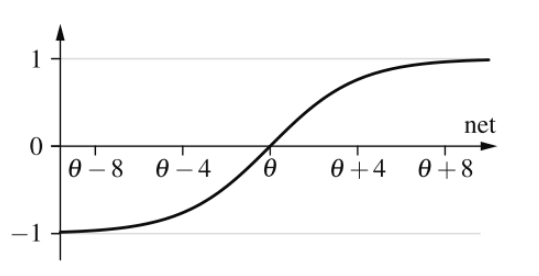
\includegraphics[width=0.48\columnwidth]{img/NN/sigmoid3}
\end{center}

Having non-linear functions allows increasing the computational capability. If all neurons had linear activation functions, having multiple hidden would be useless, you could just combine all the weights into one. With non-linear functions the more hidden layers, the more computational capabilities.\\

\newpage

Let $U_1 = \{v_1, \, ... \, , v_m \}$ and $U_2 = \{u_1, \, ... \, , u_n\}$ be the \textbf{neurons} of two \textbf{consecutive layers} of an MLP. The group of \textbf{connections between these layers} can be described by using an $n \times m$ \textbf{matrix}. The collection of the weights between the layers is: 
$$ 
W = \left(
\begin{array}{c c c c}
	w_{u_1 v_1} & w_{u_1 v_2} & ... & w_{u_1 v_m} \\
	w_{u_2 v_1} & w_{u_2 v_2} & ... & w_{u_2 v_m} \\
	... \\
	w_{u_n v_1} & w_{u_n v_2} & ... & w_{u_n v_m} 
\end{array}
\right)
$$
The computation of the network input can be written as 
$$ \vec{net}_{U_2} = \bm{W} \vec{in}_{U_2} = \bm{W} \vec{out}_{U_1} $$

An \textbf{example with the bi-implication} three-layer perceptron:
\begin{center}
	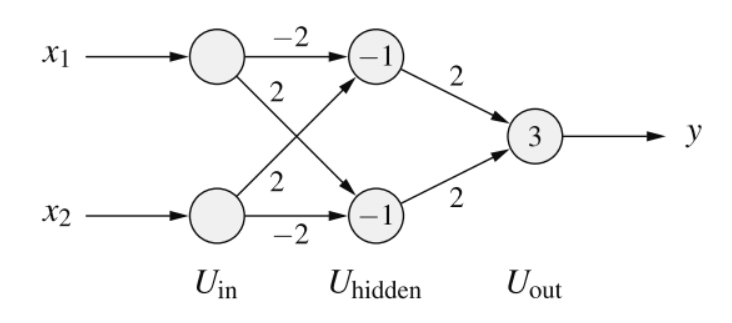
\includegraphics[width=0.65\columnwidth]{img/NN/bi_impl1}
\end{center}
Weight matrices for input and hidden layer: 
$$ \bm{W}_1 = \left(
\begin{array}{c c}
	-2 & 2 \\
	2 & -2 
\end{array}
\right)
\;\;\; \text{ and } \;\;\;
\bm{W}_2 = \left(
\begin{array}{c c}
	2 & 2 \\
\end{array}
\right)
$$

The difference between the NN and the TLU for bi-implication is that in the former we have to divide the structure into input, hidden and output layer, so we need to add a dedicated input layer.\\

\newpage

\subsubsection{Function approximation}

So far we've considered and represented only boolean functions 
$$ f: \{0,1\}^n \rightarrow \{0,1\} $$
We now want to be able to use any real number inside an MLP, so we start representing and learning \textbf{real-valued functions}
$$ f: \mathbb{R}^n \rightarrow \mathbb{R} $$

We need to demonstrate that \textbf{all Riemann-integrable functions can be approximated by four layer perceptrons} with arbitrary accuracy, provided that the output neuron has the identity, instead of a step function, as its activation function.\\

Considering this example
\begin{center}
	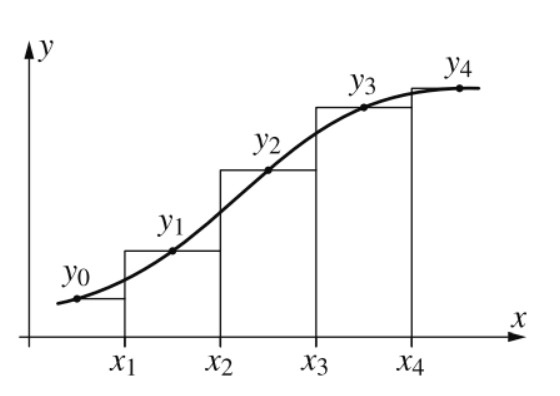
\includegraphics[width=0.5\columnwidth]{img/NN/func1}
\end{center}
We want to consider points $x_1, \, ... \, , x_4$, where we compute the value of the function, and we want to find a way to approximate a value in that function for any other $x$.\\

We can consider the \textbf{midpoint Riemann integration}: 
\begin{itemize}
	\item Approximate a given function by a step function
	\item Construct a neural network that computes said function 
	\item Error is measured as the area between functions
\end{itemize}

\newpage

This is a NN that computes the step function
\begin{center}
	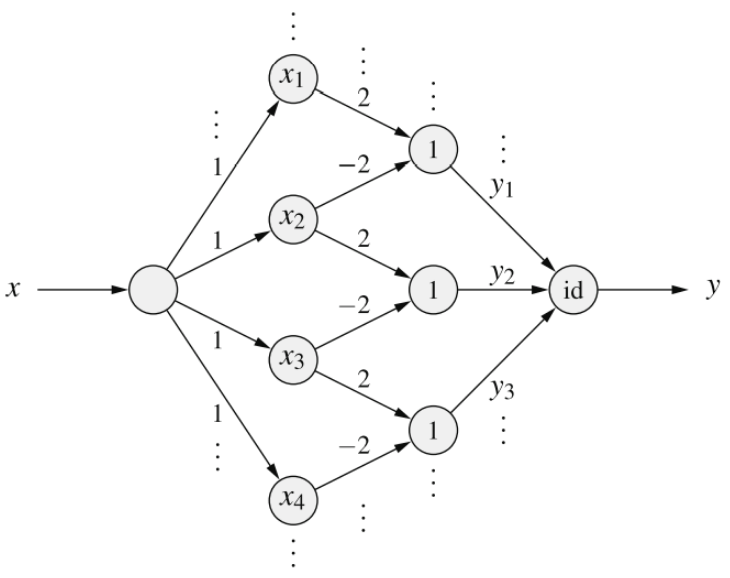
\includegraphics[width=0.7\columnwidth]{img/NN/NN2}
\end{center}

The \textbf{input} is taken by an input neuron, then the \textbf{first hidden layer} is composed of a neuron for each of the $x_i$ step borders needed for our approximation. Each of these neuron is able to determine on which side of the step border an input value lies.\\

In the \textbf{second hidden layer} we create a neuron for each step, which receives input from the two neurons in the first hidden layer that refer to the values $x_i$ and $x_{i+1}$ marking the border of the step. The neuron is activated only if the input value is less than $x_{i+1}$ and more than $x_i$, so there can be only one neuron active in the second layer; determines if the value is in the range of the step.\\

The \textbf{connections} from the neurons of the second hidden layer to the output are \textbf{weighted} with the \textbf{function values of the stair step} represented by the neurons.\\

The \textbf{output layer} receives as input only the height of the stair step in which the input value lies.\\

The \textbf{accuracy can be increased arbitrarily} by \textbf{increasing the number of steps}.

\newpage

\subsubsection{Delta approximation approach}
We can simplify this method by \textbf{considering the} $\Delta$ \textbf{variation of the function value} between each step.\\

\begin{center}
	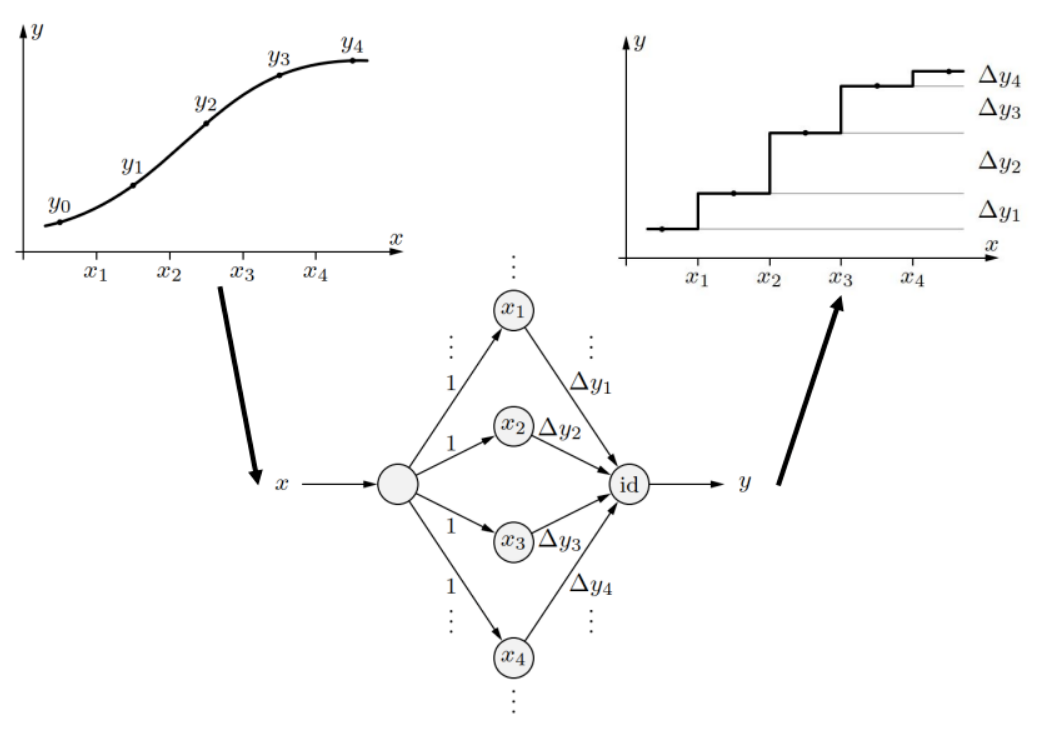
\includegraphics[width=0.9\columnwidth]{img/NN/func2}
\end{center}

This way we need only \textbf{three layers}: 
\begin{itemize}
	\item Input \\
	\item Hidden layer with a neuron for each of the $x_i$ points considered, each of these neurons determines if the input value is greater than $x_i$ (or not) \\
	\item Output \\
\end{itemize}

The \textbf{connections} between input and hidden layer are \textbf{weighted with the relative difference between each step}, so for input $x$, all neurons with a value lesser than $x$ will be active and "contribute" towards the output value.\\

% End NN L5, pag 41/42

\newpage

\subsection{Regression}
The training of neural networks is \textbf{closely related to regression}, which basically is finding the statistical model that links two variables, extrapolating a straight line that approximates the existing relationship inside a dataset.\\

All neural networks have the purpose of \textbf{minimizing the mean square error}, just like regression tries to do. We can accomplish that by adapting the weights and parameters of the activation function. This leads to the \textbf{method of least squares}, also known as \textbf{regression}, which is used to find the \textbf{best fit polynomials for a given set of data points}.\\

It will generally not be possible to find a straight line that covers exactly all $n$ points of the data set, so we have to try and find a line that deviates from these measurements as little as possible; the sum of the squared differences is minimized.\\

\subsubsection{Linear regression}
If we expect that our quantities $x$ and $y$ exhibit a linear dependence, then we have to identify the parameters $a$ and $b$ that extrapolate the line $y = g(x) = a + bx$ with as little deviation as possible.\\

Given 
\begin{itemize}
	\item a \textbf{dataset} $\left((x_1, y_1), \, ... \, , (x_n, y_n) \right)$ of $n$ data tuples
	\item a \textbf{hypothesis about the functional relationship}, e.g. 
	$$y = g(x) = a + bx$$
\end{itemize}

The approach is to \textbf{minimize the sum of squared errors}
$$ F(a,b) = \sum_{i=1}^n \left(g(x_i) - y_i \right)^2 = \sum_{i=1}^n \left(a + bx_i - y_i\right)^2 $$

\newpage

The \textbf{necessary condition to find the minimum} is having the \textbf{partial derivatives} (of the error function in respect to $a$ and $b$) \textbf{equal to 0} (\textit{Fermat's theorem})
$$ \begin{array}{c c c c}
	\displaystyle \frac{\partial F}{\partial a} & = & \displaystyle \sum_{i=1}^n 2 \left(a + b x_i - y_i \right) & = 0 \\
	\hfill \\
	\displaystyle \frac{\partial F}{\partial b} & = & \displaystyle \sum_{i=1}^n 2 \left(a + b x_i - y_i \right)x_i & = 0
\end{array} $$
The system \textbf{can be solved} with standard methods from linear algebra and the \textbf{solution is unique}, unless all values of $x$ coincide (trivial, the data would be useless), in which case there are infinite solutions.\\

\paragraph{Example:} starting from these points
\begin{center}
	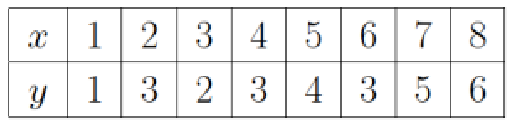
\includegraphics[width=0.45\columnwidth]{img/NN/linreg1}
\end{center}
The regression line would become
$$ y = \frac{3}{4} + \frac{7}{12} x $$
\begin{center}
	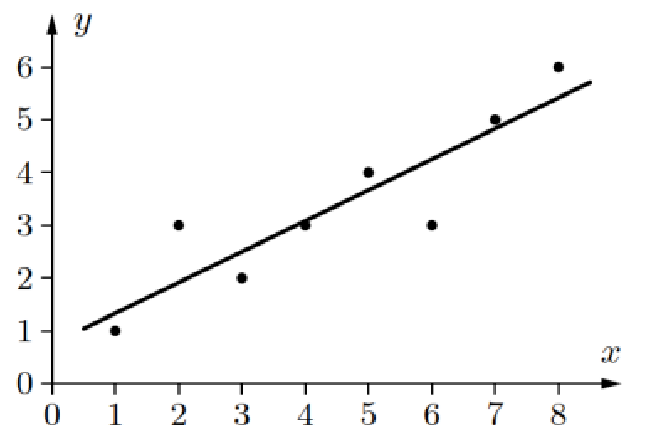
\includegraphics[width=0.5\columnwidth]{img/NN/linreg2}
\end{center}

\newpage

\subsubsection{Polynomial regression}
The previous method can be extended to \textbf{polynomial of arbitrary order}. Instead of considering a grade equal to one, we consider a polynomial of grade $m$: 
$$ y = p(x) = a_0 + a_1 x + \, ... \, + a_m x^m $$

The \textbf{minimization} for the sum of squared \textbf{errors} can be generalized into
$$ F(a_0, a_1, \, ... \, , a_m) = \sum_{i=1}^n \left(p(x_i) - y_i\right)^2 = \sum_{i=1}^n (a_0 + a_1 x_1 + \, ... \, + a_m x_i^m - y_i)^2 $$

The necessary \textbf{conditions for a minimum} are that \textbf{all partial derivatives vanish}
$$ \frac{\partial F}{\partial a_0} = 0, \; \frac{\partial F}{\partial a_1} = 0, \;\; ... \;\; , \frac{\partial F}{\partial a_m} = 0 $$
It can be solved with standard methods just like before, the \textbf{solution is} also \textbf{unique}, unless the points lie exactly on a polynomial of lower degree (another trivial case).\\

\newpage

\subsubsection{Multi-linear regression}
We can \textbf{generalize} the previous methods to \textbf{more than one argument}
$$ z = f(x,y) = a + bx + cy $$

We're applying linear regression to multiple variables, the concept is the same as before but multi-linear.\\

We need to \textbf{minimize the sum of squared errors}, the difference between the function $f$ and the sample values $z_i$
$$ F(a,b,c) = \sum_{i=1}^n \left(f (x_i, y_i) - z_i \right)^2 = \sum_{i=1}^n \left(a + b x_i + c y_i - z_i \right)^2 $$

Like before, for a \textbf{minimum} we need \textbf{all partial derivatives} to \textbf{vanish}
$$ \begin{array}{c c c c}
	\displaystyle \frac{\partial F}{\partial a} & = & \displaystyle \sum_{i=1}^n 2 \left(a + b x_i + c y_i - z_i \right) & = 0, \\
	\hfill \\
	\displaystyle \frac{\partial F}{\partial b} & = & \displaystyle \sum_{i=1}^n 2 \left(a + b x_i + c y_i - z_i \right)x_i & = 0, \\
	\hfill \\
	\displaystyle \frac{\partial F}{\partial c} & = & \displaystyle \sum_{i=1}^n 2 \left(a + b x_i + c y_i - z_i \right)y_i & = 0
\end{array} $$
As before, \textbf{can be solved} and \textbf{solution is unique} unless all data points lie on a straight line (there's a plane that can be rotated in any direction and thus infinite solutions).\\

\newpage

We can also have a \textbf{general multi-linear case} with a \textbf{function} defined on $m$ \textbf{variables} (there aren't enough dimensions to draw this)
$$ y = f(x_1, \, ... \, , x_m) = a_0 + \sum_{k=1}^m a_k x_k $$

\textbf{Minimize} the \textbf{sum of squared errors}
$$ F (\vec{a}) = \left(\bm{X} \vec{a} - \vec{y}\right)^{\top} \left(\bm{X} \vec{a} - \vec{y}\right)$$

Where
$$ 
\bm{X} = \left(
\begin{array}{c c c c}
	1 & x_{11} & ... & x_{m1} \\
	... \\
	1 & x_{1n} & ... & x_{mn}
\end{array}
\right), \;\;
\vec{y} = \left(
\begin{array}{c}
	y_1 \\
	...\\
	y_n
\end{array}
\right), \;\;
\vec{a} = \left(
\begin{array}{c}
	a_0\\
	a_1\\
	...\\
	a_m
\end{array}
\right)
$$
We have vectors for the parameters and matrices to define the values.\\

Necessary conditions for a minimum
$$ \vec{\nabla}_{\vec{a}} F(\vec{a}) = \vec{\nabla}_{\vec{a}} \left(\bm{X} \vec{a} - \vec{y}\right)^{\top} \left(\bm{X} \vec{a} - \vec{y}\right) = \vec{0} $$
I need to define the \textbf{gradient}, generalization of the partial derivatives on vectors. We need to find where the gradient is 0, which will give us the hyperplane touching the surface in the minimum (kinda like before but not a line, it's a plane in fuck-knows how many dimensions, I guess).\\

This comes out to a set of regular equations
$$ \bm{X}^{\top} \bm{X} \vec{a} = \bm{X}^{\top} \vec{y} $$
which has a solution, unless $\bm{X}^{\top} \bm{X}$ is singular 
$$ \vec{a} = \left(\bm{X}^{\top} \bm{X}\right)^{-1} \bm{X}^{\top} \vec{y} $$

\vfill 

This last subsubsection has been discussed very roughly, no need to understand the math exactly (I hope).

\newpage

\subsubsection{Logistic regression}
It's reasonable to assume that Neural Network want to use non-linear, and in general non-polynomial functions, so we want to be able to approximate a dataset with \textbf{different types of functions}, for example
$$ y = ax^b$$

We can find a \textbf{transformation to a linear/polynomial case}
$$ \ln y = \ln a + b \ln x $$

In the case of an ANN we are interested in the \textbf{logistic function}
$$ y = \frac{Y}{1 + e^{a+bx}} $$ 

A lot of ANNs use the logistic function as activation, so being able to do linear regression on that would mean being able to effectively determine any parameter of any network.\\

We can derive from this equation, using a logarithm, a \textbf{linear description}; we go from a non-polynomial function to a linear one, to be able to minimize the sum of squared errors. The value $a$ of the function represents the threshold of the output neuron, while the value of $b$ represent the weight of the input. \\

We can linearize the logistic function by way of the \textbf{Logit-transformation}
$$ y = \frac{Y}{1 + e^{a+bx}} \Leftrightarrow \frac{Y - y}{y} = e^{a + bx} \Leftrightarrow \ln \left(\frac{Y - y}{y}\right) = a + bx $$

\newpage

Example:
\begin{center}
	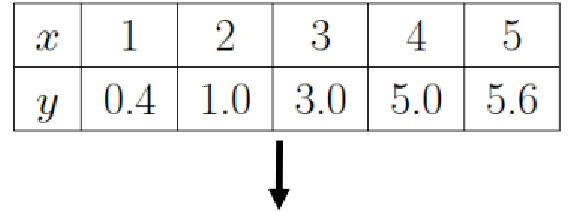
\includegraphics[width=0.4\columnwidth]{img/NN/logreg1}
\end{center}
$$ z = \ln \left(\frac{Y - y}{y}\right), \;\;\;\; Y = 6$$
\begin{center}
	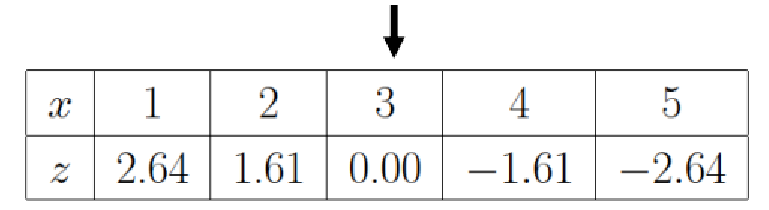
\includegraphics[width=0.55\columnwidth]{img/NN/logreg2}
\end{center}
The results of the regression line in the example are:
$$ z \approx -1.3775x + 4.133 \;\;\;\; y \approx \frac{6}{1 + e^{-1.3775x} + 4.133} $$

Plot of logistic functions: 
\begin{center}
	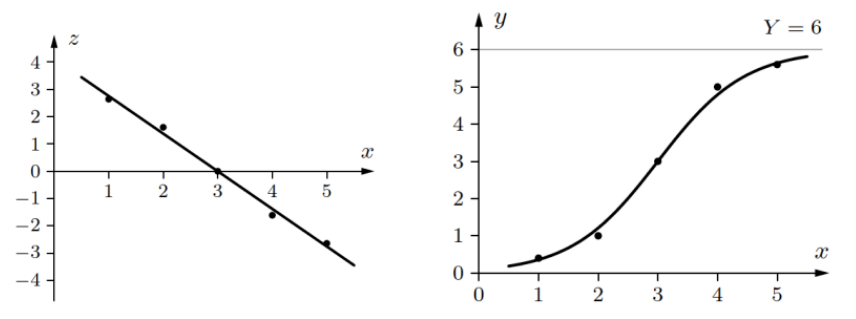
\includegraphics[width=0.9\columnwidth]{img/NN/logreg3}
\end{center}
The logistic regression function can be computed by a single neuron.\\

If we can find a method to determine a logistic regression function, we immediately possess a method to determine the parameters of a two-layered perceptron with a single input.\\

\vfill

As before, the initial concepts are important, the exact math and consequences are not (I hope, they're being explained like they're not).

\newpage

\subsubsection{Two-class problems}
Going from the regression part to the classification (binary, in this case). The idea is to \textbf{model the conditional probability of one class as a logistic function}. I have a function, the two classes are divided by the line (value over the function are class 0, under are class 1).\\

Let $C$ be a \textbf{class of attributes} and $\dom (C) = \left\{c_1, c_2\right\}$ and $\vec{X}$ a \textbf{random vector} in $m$ dimensions.\\

Given a set of \textbf{data points} $X = \left\{\vec{x}_1 , \, ... \, , \vec{x}_n \right\}$ each of which belongs to one of the two classes $c_1$ and $c_2$.\\

We consider the \textbf{probability} of belonging to the first class $c_1$ and the probability to be in the second class $c_2$
$$ P (C = c_1 | \vec{X} = \vec{x}) = p(\vec{x}) $$
$$ P (C = c_2 | \vec{X} = \vec{x}) = 1 - p(\vec{x}) $$

We want to obtain a \textbf{simple description of the function} $p(\vec{x})$, we can describe it by a logistic function
$$ p(\vec{x}) = \frac{1}{1 + e^{a_0 + \vec{a} \vec{x}}} = \frac{1}{1 + \exp \left(a_0 + \sum_{i=1}^m a_i x_i \right)} $$

Then we can apply the \textbf{logit transformation} so that we can obtain the formal description of the \textbf{probability of being on one or the other class}:
$$ \ln \left(\frac{1 - p(\vec{x})}{p (\vec{x})}\right) = a_0 + \vec{a} \vec{x} = a_0 + \sum_{i=1}^m a_i x_i $$

\textit{How can we find the specific value of the probability (and thus solving the splitting of the example)?} We can consider a specific function called \textbf{kernel} that describes how strongly a data point influences the probability estimate for neighboring points. This gives us correlation among elements of the same class.\\

\newpage

With a kernel we can describe the similarity of a group of examples, the Gaussian function is commonly used. This function increases as the data point considered approaches the middle (the sample is similar to both groups, it's in the middle, value is high) and decreases the further I go
$$ K (\vec{x}, \vec{y}) = \frac{1}{2 \pi \sigma^2} \exp \left(- \frac{(\vec{x} - \vec{y})^{\top} (\vec{x} - \vec{y})}{2 \sigma^2}\right)$$

If we want to estimate the \textbf{probability density} the expression is
$$ \hat{f} (\vec{x}) = \frac{1}{n} \sum_{i=1}^n K(\vec{x}, \vec{x}_i)$$

The kernel estimation applied to a two-class problem:
$$ \hat{p} (\vec{x}) = \frac{\sum_{i=1}^n c(\vec{x}_i) K(\vec{x}, \vec{x}_i)}{\sum_{i=1}^n \vec{x}_i}$$

If it is
$$ c(\vec{x}) = 1 $$
the $x_i$ will belong to class $c_1$, to the remaining class otherwise.\\

\vfill

This page is NOT found in the lesson, it's from external sources.

\newpage

This classification model allows us to obtain the parameters via \textbf{maximizing the likelihood of the data}, we choose the \textbf{parameters} that \textbf{make the data most likely} by setting up a \textbf{likelihood function} which describes how probable the given data is depending on the parameters.\\

With this approach, we can apply the classification rule to new data: 
$$ C = c_1 \text{ if } p(x, a) \geq \theta $$
$$ C = c_0 \text{ if } p(x, a) < \theta $$
With $\theta = 0.5$.\\

We now can, in theory, proceed with a linear regression: a necessary condition for a \textbf{minimum of the negative log likelihood is that its gradient vanishes}.\\

The resulting equation system is not linear and difficult to solve analytically, we need to consider a \textbf{gradient descent}.\\

\vfill 

TLDR(?): We transform the non-polynomial function into a linear case, then we can apply the minimization of the sum of squared errors to get a solution. Then the output of the two classes is obtained by putting a threshold the output, over it's one class, under it's the other. We have $x$ and the corresponding $y$, but there's an extra step, we need to consider a threshold on the result, over it's one class, under it's the other.\\

(this is based on what he's saying, this man is cray-cray)

% End of NN L6 (orcodio peggiora sempre di più, sta diventando un casino seguirlo sto qua)

\newpage

\subsection{Training MLPs}
\subsubsection{Gradient descent}
Logistic regression would work, but only for two-layer perceptrons, so the general approach is \textbf{gradient descent}.\\

If we can derive from the error function in which direction we have to change the weights and bias the values in order to reduce the error, we obtain a possibility to train the parameters of the network. The average error across all neurons will determine the overall "quality" of our network. \\
We make small steps into these directions, check the directions again and repeat the process.\\

We modify the values of the parameters one step at a time and check if the error is reduced (we're converging). We do this since a purely analytical solution would be hard to find. The requirement is to have \textbf{differentiable activation and output function}; this means that, in this case, the error function will be differentiable as well and thus we can determine the directions we need to minimize the error function.\\

The input that minimizes the cost of our error function is the one that gives $\frac{d}{dw} e(w) = 0$, but this is not really feasible for complicated functions, so we can find a \textbf{local minimum} (global minimum is also pretty hard).\\

This concept has to be translated to a scenario with multiple parameters (we have weights, biases and stuff). If we have two variables the error function can be graphed as a surface along the $xy$ plane; to minimize it we need to ask \textit{in which direction the error function decreases more quickly?} And multi-variable calculus has the concept of \textbf{gradient} as an answer, defined as the direction of the steepest increase $\vec{\nabla} e(x,y)$ and the length of the vector determines how steep is the increment.\\

The algorithm will essentially be: 
\begin{itemize}
	\item Compute $\vec{\nabla} e(x,y)$
	\item Small step in direction $- \vec{\nabla} e(x,y)$
	\item Repeat until convergence
\end{itemize}
The negative gradient determines how the weights and biases need to be modified to efficiently decrease the cost. The backpropagation is an algorithm for computing that gradient.\\

The gradient is a vector expressed in $n$-dimensions, where $n$ depends on the weights and biases, usually it's a giant number (impossible to visualize). The important thing is the magnitude of each component (so the value) since it will make us able to determine \textbf{how sensitive} the error function output will be respect to the weight and bias (how much it moves respect the previous value). \\

We need to apply this for all the values of the weights of a network. Essentially when we talk about \textbf{training} or the process of learning of a NN it's just about \textbf{minimizing the error function}. More to that, the negative gradient vector will store the relative importance of the weights for each neuron (how important each neuron is for the total error, this is a value needed for the backpropagation). The gradient of a real-valued function is the set of all partial derivatives. Intuitive interpretation of the gradient of a real-valued function $z = f (x, y)$ at a point $(x_0, y_0)$:
\begin{center}
	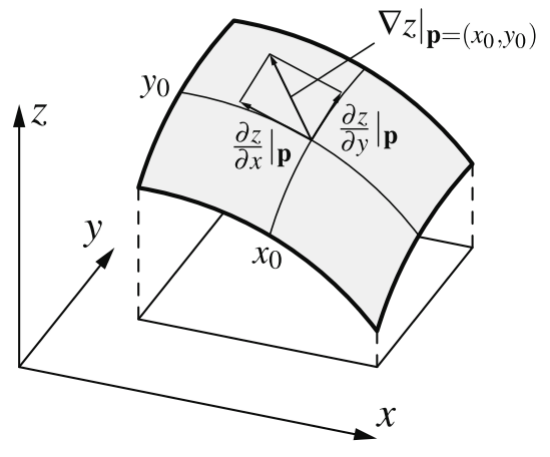
\includegraphics[width=0.5\columnwidth]{img/NN/gradient1}
\end{center}

Training becomes very simple: the weights and bias \textbf{values are initialized randomly} and then the \textbf{gradient} of the error function \textbf{is computed} at the point given by these values.\\

\newpage

The solution to our learning process is given by \textbf{reaching the minimum of the error function}, one small \textbf{step} at a time, in the \textbf{direction opposite to the gradient}. At the new point we recompute the gradient until a minimum is reached.
$$ e = \sum_{l \in L_{fixed}} e^{(l)} = \sum_{v \in U_{out}} e_v = \sum_{l \in L_{fixed}} \sum_{v \in U_{out}} e_v^{(l)} $$
The \textbf{sum of the individual errors over all output neurons} $v \in U_{{out}}$ \textbf{and all training patterns} $l \in L_{fixed}$.\\

So we need to evaluate the gradient in order to go in the proper direction. In the case of an MLP calculating the gradient means computing the partial derivative of the error function in respect of the threshold and the weights taken as parameters.\\

Given $\vec{w}_u = (-\theta, w_{u_1}, \, ... \, , w_{u_k})$ as the vector of weights of a single layer extended with the threshold, then the \textbf{gradient is computed as follows}:
$$ \vec{\nabla}_{\vec{w}_u} e = \frac{\partial e}{\partial \vec{w}_u} = \left(- \frac{\partial e}{\partial \theta_u}, \frac{\partial e}{\partial w_{up_1}}, \, ... \, , \frac{\partial e}{\partial w_{up_n}}\right) $$

The total error $e$ is given by the sum of individual errors across all neurons and training patterns, so we get: 
$$ \vec{\nabla}_{\vec{w}_u} e = \frac{\partial e}{\partial \vec{w}_u} = \frac{\partial }{\partial \vec{w}_u} \sum_{l \in L_{fixed}} e^{(l)} = \sum_{l \in L_{fixed}} \frac{\partial e^{(l)}}{\partial \vec{w}_u} $$ 

\newpage

Considering the logistic function and its derivative
$$ f_{act} (net_u^{(l)}) = \frac{1}{1 + e^{- net_u^{(l)}}} \;\;\;\;\;\;\;\;\;\; f_{net}' (net_u^{(l)}) =  f_{act} (net_u^{(l)})$$  
\begin{center}
	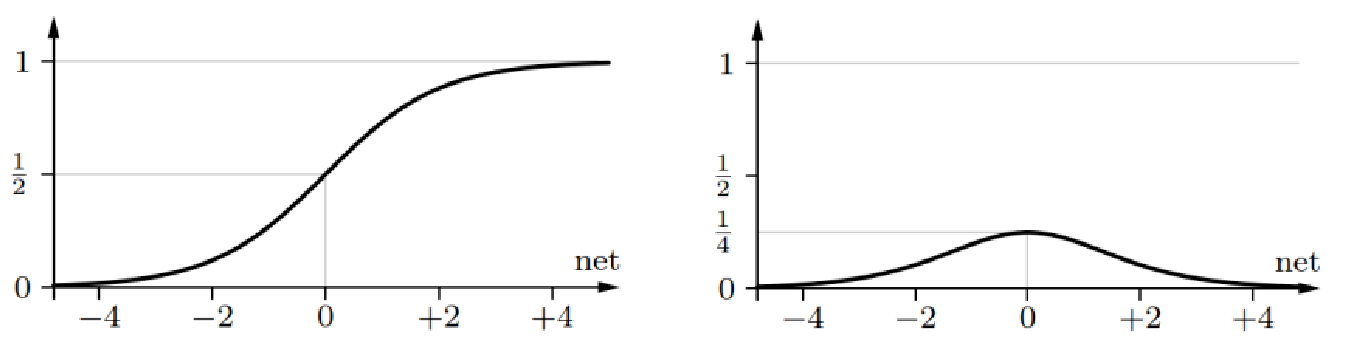
\includegraphics[width=0.9\columnwidth]{img/NN/logfunc1}
\end{center}

The \textbf{weight changes} (performed on the vector $\vec{w}_u$) are \textbf{proportional to the derivative} of function $f_{act}' (net_u^{(l)})$
\begin{itemize}
	\item Close to 0 weight changes (and thus training speed) are at the highest
	\item Far from 0 the gradient becomes small and training slow
\end{itemize}

Gradient descent may be more or less effective depending on the landscape of the error function. We need to find the minimum, if the function is steeper small steps give significant changes, otherwise you'll need more steps.\\

\newpage

\subsubsection{Error backpropagation}
So far, only the output neurons are directly connected to the error, they're the only one that can see "how wrong they are". But we \textbf{need to train the whole network}.\\

For the last layer we can see the error, and thus we can compute the change directly, it's the derivative of the error function with respect to the weight of the neuron.\\
But what about the layers previous to the last one? We do kinda the same thing, but how much I modified the last layer becomes the error for the second to last one. The partial derivative to that error gives how much we have to modify that layer.\\
The process can repeat for all layers.\\

The error values of any (hidden) layer of an MLP can be computed from the error values of its successor. The sum of the errors of the weights of the last layer becomes the error function to minimize for the weights of the layer before that.\\

The error is computed at the end of the network and then \textbf{backpropagated}, we need to modify all the weights in the network. The error signal is transmitted from the output layer backwards.\\

\newpage

General structure: 
\begin{enumerate}
	\begin{tcolorbox}[colback=white, colframe=green]
		\item Setting the input 
		$$ \forall i \in U_{in} : \, out_u^{(l)} = ext_u^{(l)} $$
		We're just giving the inputs.\\
	\end{tcolorbox}
	
	\begin{tcolorbox}[colback=white, colframe=blue]
		\item Forward propagation of the input
		$$ \forall u \in U_{hidden} \cup U_{out} : \, out_u^{(l)} = \left(1 + exp \left(- \sum_{p \in pred(u)} w_{up} out_p^{(l)}\right)\right)^{-1} $$
		We process the inputs until we get an output, this is the "work phase". \\
	\end{tcolorbox}
	
	\begin{tcolorbox}[colback=white, colframe=red]
		\item Error factor
		$$ \forall u \in U_{out}: \, \delta_u^{(l)} = \left(o_i^{(l)} - out_u^{(l)} \right) \lambda_u^{(l)} $$
		We compute the error for the last layer (basically just the difference between output obtained and desired). \\
	\end{tcolorbox}
	\begin{tcolorbox}[colback=cyan, colframe=black]
		Weight adaptation
		$$ \Delta w_{up}^{(l)} = \eta\delta_u^{(l)} out_p^{(l)} $$
	\end{tcolorbox}
	
	\begin{tcolorbox}[colback=white, colframe=yellow]
		\item Error Backpropagation
		$$ \forall u \in U_{hidden}: \, \delta_u^{(l)} = \left(\sum_{s \in succ(u)} \delta_s^{(l)} w_{su}\right) \lambda_u^{(l)} $$
		The "new" error factor is computed starting from the error of the subsequent layer.\\
	\end{tcolorbox}
	\begin{tcolorbox}[colback=white, colframe=black]
		Derivative of the activation function
		$$ \forall u \in U_{hidden} \cup U_{out}: \, \lambda_u^{(l)} = out_u^{(l)} \left(1 - out_u^{(l)}\right) $$
	\end{tcolorbox}
	% We have to compute the partial derivative of the error in respect to the weight, in order to know by how much we need to change the weight. Repeat this step. \\
\end{enumerate}
\begin{center}
	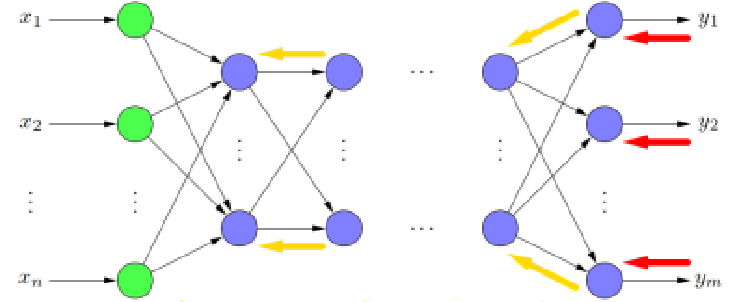
\includegraphics[width=0.9\columnwidth]{img/NN/backprop1}
\end{center}

\newpage

Another explanation (since the last one was shit): We assume that the \textbf{activation function a logistic function for each neuron} $u \in U_{hidden} \cup U_{out}$, except for the input neurons.
\begin{enumerate}
	\item \textbf{Apply the input} at the input neurons that is returned without modifications at the subsequent first hidden layer (just give the inputs man). \\
	
	\item We \textbf{compute} for each neuron of the subsequent layers the weighted sum of the inputs, applying at the result our logistic function, \textbf{producing the output that will be propagated} throughout the network until the terminal neurons (elaborate the inputs).\\
	
	\item \textbf{Compute the difference between the desired output and the actual output}. Since it's possible to invert the logistic function $f_{act}$, we can know which was the input (error) that has induced that particular error ($\delta_u$).\\
	
	\item Now that we have transformed the error of the output variable $out_u$ in the error of the input variable $net_u$, we can \textbf{distribute the error} (with the correction) in a proportional way back to previous neuron, we \textbf{backpropagate} the error until the input neurons.\\
\end{enumerate}

We have to say that given the shape of the logistic function the error can disappear completely, since the gradient will approximate more the \textbf{null vector} the more it will be near the zero. \\

The \textbf{weight adaptation} is performed by the following \textbf{formula} (this tells how to perform the correction):
$$ \forall w_{up} : \, \delta w_{up} = \eta \delta_u out_p $$

If you initialize the \textbf{learning rate} $\eta$ with too high of a value, instead of descending the curve we risk jumping from a "peak" of the function to another (jumps over the minimum), without ever converging to the minimum. Furthermore, it's NOT certain that the minimum reached in this way is the global minimum of the function. \\

A \textbf{solution} to the problem could consist in \textbf{repeating the learning}, initializing the system with a different configuration of weights and threshold, and then choose at the end which configuration results in the better minimum.\\

On the contrary, a value too small for $\eta$ makes the learning too long and takes too many steps. The correct value has to be chosen through trial and error (mostly by vibes I guess).\\

%\newpage

\paragraph{Negation example:} considering the negation $\neg x$, there's a two layer perceptron for said function
\begin{center}
	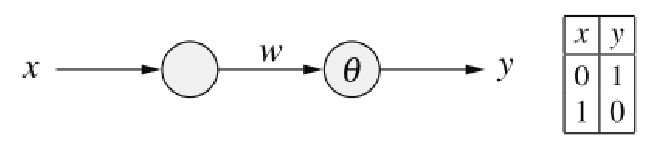
\includegraphics[width=0.5\columnwidth]{img/NN/neg1}
\end{center}
By using the logistic activation function we get these squared errors for computing the negation:
\begin{center}
	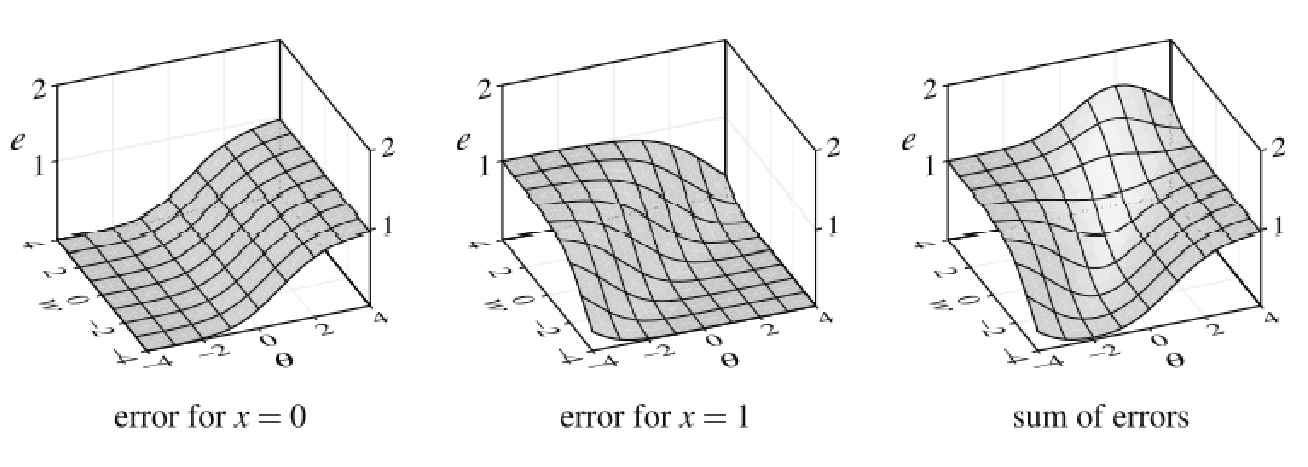
\includegraphics[width=0.9\columnwidth]{img/NN/neg2}
\end{center}

From a numeric point of view, the error \textbf{can't completely vanish due to the properties of the logistic function}, there will always be some residual errors due to the computation of the various parameters. The error keeps getting smaller and smaller but it doesn't vanish completely.\\

\newpage

\subsubsection{Variants of Gradient Descent}
There can be \textbf{variants} of the gradient descent: 
\begin{itemize}
	\item \textit{Manhattan training}, considers only the sign of the gradient, fast but might not reach the optimum.\\
	\item \textit{Flat spot elimination}, the derivative of the action function is lifted by a certain value $\alpha$ so that sufficiently large training steps are taken even in flat spot regions.\\
	\item \textit{Momentum term}, at each step a fraction of the preceding weight change is added to a normal gradient descent step.\\
	\item \textit{Self-adaptive error backpropagation}, each parameter has a different learning rate, allowing a finer control of the learning process.\\
	\item \textit{Resilient error backpropagation}, combination of the Manhattan training with the Self-adaptive error backpropagation.\\
	\item \textit{Quick propagation}, instead of using the gradient, approximate the error function to a parabola and jump to the peak.\\
	\item \textit{Weight decay}, reduce the weight to prevent getting stuck in the saturation region .\\
\end{itemize}
A common combination to avoid overfitting and keeping the absolute value of the weights as little as possible is Momentum term and Weight decay.\\

\newpage

\subsection{Number of hidden neurons}
The \textbf{number} of \textbf{input neurons} is \textbf{dependent on the data} (10 features, 10 neurons), the \textbf{number} of \textbf{output neurons} depends on the \textbf{type of problem} considered (10 classes, 10 neurons).\\

There's \textbf{no fixed rule for the number of neurons in hidden layers}, the process should consist of increasing the number (and thus the capabilities of the network) until there's overfitting (the network is also learning the error in the data).\\

For a \textbf{single hidden layer} the following rule of thumb is popular: 
$$ \text{Number of hidden neurons} = \frac{\text{number of inputs} + \text{number of outputs}}{2}$$

\paragraph{Underfitting:} the number of neurons in the hidden layer is too small, the MLP may not be able to correctly approximate the function (and thus the relation between input and output values) due to a lack of parameters.\\

\paragraph{Overfitting:} the number of neurons in the hidden layer is too big, the MLP learns too much from the examples and the abundance of parameters allows it to fit exactly the training data given, error included, leading to a loss in the ability of generalizing the desired behavior. It's learning the error in the data along the data itself.\\

\newpage

\subsection{Cross Validation}
We need to \textbf{evaluate the performance of the network} (is the training good?). The objective is training the model on some data, and it should perform correctly on new data. \\

To understand the quality of training we split our data in two subsets: 
\begin{itemize}
	\item \textbf{Training set:} used for training
	\item \textbf{Validation set:} used for checking the quality of the result
\end{itemize}
This allows us to see if the NN is overfitting the training data and evaluate the general quality of the learning. \\

If I increase the neurons and get a lower error on the validation, I'm still underfitting (needs more neurons, more capabilities), while if I increase the capabilities and get a higher error, the NN is overfitting.\\

The \textbf{cross validation} consists in training different MLPs with different numbers of hidden neurons and evaluate them with the two subsets, multiple times with the data randomly split across training and evaluation, averaging the results for each "number of neurons". At the end the number of neurons with the lowest average error is chosen.\\

\newpage

\subsubsection{N-Fold Cross validation} 

Another method to evaluate training
\begin{itemize}
	\item The given \textbf{data set is split into} $n$ \textbf{parts} or subsets (also \textbf{called folds}) of about equal size
	\item The relative frequency of the output values in the subsets/folds represents as well as possible the relative frequencies of these values in the data set as a whole (\textbf{stratification})
	\item Out of these $n$ data folds, $n$ \textbf{pairs of training and validation data sets are formed} by using one fold as validation and $n-1$ folds for training
\end{itemize}

This way, \textbf{we train the model for each one of the} $n$ \textbf{training sets}, avoiding overfitting problems and asymmetric sampling typical of the classic cross validation. In other words the sample is subdivided in group of equal size, one group at time is excluded (this is predicted by using the non excluded groups), in order to evaluate the prediction model used. \\

Basically, out of $n$ folds, 1 is kept for validation, the other for training and repeat $n$ times, each time with a different validation fold.\\

The \textbf{stopping criterion} is also important, the training continues as long as the error decreases, it stops as soon as the error increases (start of overfitting).\\

% End NN L7 (una settimana per sta merda)

\newpage

\subsubsection{Sensitivity analysis}
The great capabilities of NNs also make it difficult to understand exactly what they're doing, the \textbf{knowledge learned} is often \textbf{encoded in matrices/vectors} of real-valued numbers, often \textbf{difficult to understand or extract}. Geometric interpretation are only possible for very simple networks. A NN effectively becomes a \textit{black box}.\\

We have no real way to know what's inside the network, but we can have a \textbf{sensitivity analysis} can be useful to find out \textbf{to which inputs the output(s) react(s) most sensitively}; we want to find out what parts of the input influence the output and how. This can give information about which inputs are not needed and may be discarded. Basically we want to answer \textit{"How much the output of each neuron is changing if we change
	the data set for training (still describing the desired behavior)?"}.\\

The approach is to \textbf{determine the change of output relative to the change of input}:
$$ \forall u \in U_{in}: \;\; s(u) = \frac{1}{|L_{fixed}|} \sum_{l \in L_{fixed}} \sum_{v \in U_{out}} \frac{\partial out_v^{(l)}}{\partial ext_u^{(l)}} $$

This allows us to have an idea of what the NN is using to make a certain decision, which inputs are more important than others.\\

% End of NN L8 (letteralmente mezz'ora per far tutto, fantastico), appunti 57

\newpage

\subsection{Deep Learning}
"Deep Learning" refers to a NN with \textbf{several hidden layers}. With "\textit{depth}" we mean the highest possible number of layers that separate input and output (longest path in the network graph).\\

An MLP with three layers (one hidden layer) can approximate arbitrarily well any continuous integrable function (\textbf{universal approximation theorem}), but depending on the function, a very large quantity of neurons (e.g. exponential in the number of inputs) may be necessary. Allowing for \textbf{more hidden layers} may enable to achieve the \textbf{same approximation quality with a significantly lower number of neuron}.\\

\paragraph{Example:} considering the $n$-bit parity function, which outputs 1 only if an even number of inputs is 1, if we want to approximate this function with a single hidden layer we'd need $2^{n-1}$ neurons, and this number (clearly) \textbf{grows exponentially} with the number of inputs. \\

With multiple hidden layers, \textbf{linear growth is possible}:
\begin{center}
	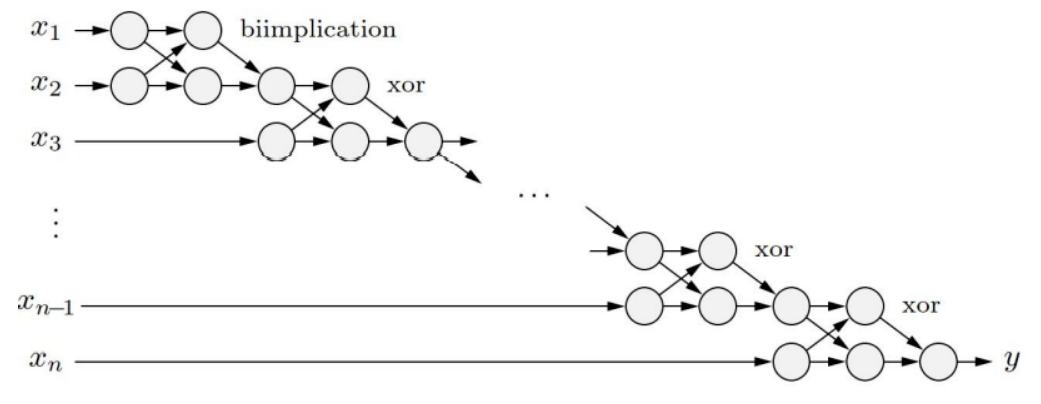
\includegraphics[width=0.95\columnwidth]{img/NN/nbitparity1}
\end{center}
(this example allows for as many hidden layers as needed).\\
The disjunctive normal for of this function is composed of $2^{n-1}$ conjunctions, i.e. the number of combinations with an even number of set bits, this makes the number of hidden neurons grow exponentially.\\
If we're allowed to use more than one hidden layer, we can construct an MLP that chains together $n-1$ simple networks for computing the biimplication (which basically is a $n$-bit parity on 2 bits). The number of neurons increases to $n(n+1)-1$.

\newpage

The concept is that \textbf{increasing the number of hidden layers can decrease the complexity required}.\\

Another motivation for DNN is that \textbf{training data sets are limited in size}. A complete training data for any $n$-ary boolean function has $2^n$ training examples and in practical problems usually there are much fewer sample cases. Reducing the number of neurons allows us to use data sets limited in size (less stuff to train I guess).\\

\paragraph{Main problems:} while having deeper network can help they may also pose some problems:
\begin{itemize}
	\item \textbf{Overfitting:} we're increasing the number of adaptable parameters and thus increasing capabilities, this can lead to overfitting the sample data
	\item \textbf{Vanishing gradient:} the gradient tends to vanish if many layers are backpropagated through and learning in the early hidden layers can become very slow, it gets smaller and smaller as you get towards the input
\end{itemize}

There are some possible \textbf{solutions to the overfitting} issue: 
\begin{itemize}
	\item \textbf{Weight decay:} avoid large values for the weights to prevent an overly precise adaptation
	\item \textbf{Sparsity constraints:} restrict the number of neurons in hidden layers, thus removing some connections, or require that only few of the neurons in the hidden layers should be active (on average)
	\item \textbf{Dropout training:} during training, some units are randomly omitted from the input/hidden layers (for both forward and backward propagation), the network is not fully connected
\end{itemize}

For the vanishing gradient, in principle, it could be counteracted by a large weight, but this leads to overfitting and saturation of the activation functions.\\

\newpage

For the \textbf{vanishing gradient, solutions}:
\begin{itemize}
	\item Obviously we can "brute force" it and increase the size of the training set, the number of epoch. It has some clear drawbacks, but as computational power increases this becomes more feasible.\\
	
	\item \textbf{Other activation functions} limit the problem of vanishing gradient, functions that have higher values of the gradient for a broader range of values, such as hyperbolic tangent, ReLUs and variations, softplus, ecc.; the point is \textbf{having large values of the gradient, close to 1, for larger ranges of inputs}, to avoid the gradient vanishing too fast.\\
	
	\item Another approach is \textbf{training the NN layer by layer}, training only the newly added layer in each step. A popular way of doing this is building the network as \textbf{stacked autoencoders}. An autoencoder is a 3-layer perceptron that \textbf{maps its inputs to approximations of themselves}. The hidden layer forms an encoder into some form of representation and the output layer forms a decoder that (approximately) reconstructs the inputs. It's trained to reconstruct itself, but the hidden layer is smaller so the encoder is forced to learn a meaningful representation of the input features. The hidden layer is expected to construct features.
	\begin{center}
		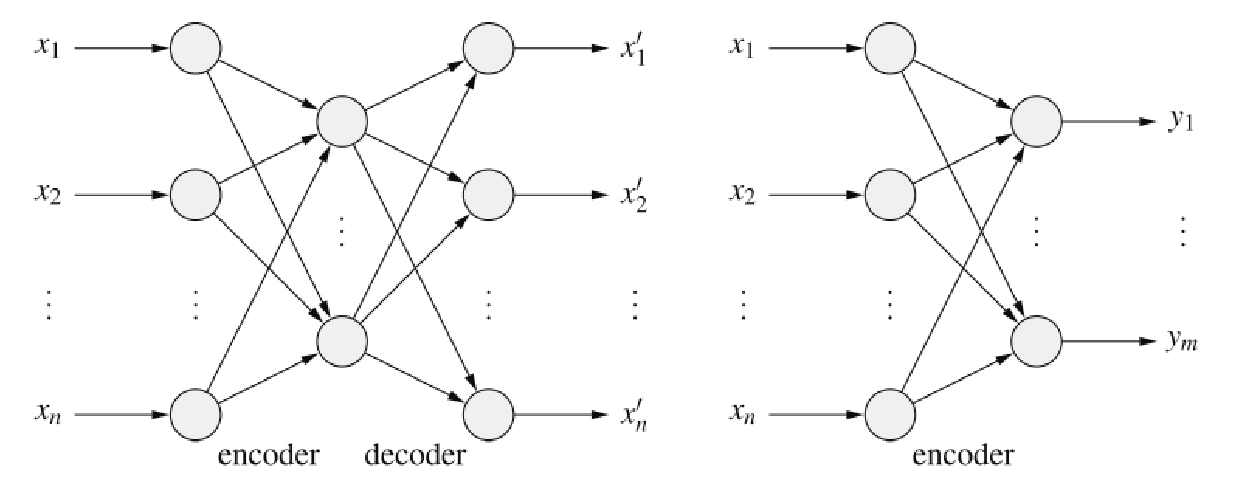
\includegraphics[width=0.9\columnwidth]{img/NN/autoencoder}
	\end{center}
	After the first encoder, I remove the decoder layer and add another hidden layer, only this last one added has to be trained, since we kept the already trained encoder part from before. Each encoder can be trained normally with backpropagation.\\
	
	\newpage
	
	Problem: if there are \textbf{as many (or even more) hidden units as there are inputs} it's likely that the \textbf{input will propagate with little to no adjustments} to the output. We need to keep a limited number of neurons. Solutions: 
	\begin{itemize}
		\item \textbf{Sparse auto-encoders:} provide a (considerably) smaller number of hidden neurons compared to the input layers. 
		
		\item \textbf{Sparse activation scheme:} the number of active neurons in the hidden layer is restricted to a small number. Force sparsity constraints, add in the error function what is basically the number of active neurons so that the training will try to minimize such number.
		
		\item \textbf{Denoising autoencoders:} add noise to the input (but not to the data used for evaluation) and train the autoencoder to reconstruct the clean version, this way the input can't simply "pass through".
		
		%force sparsity constraints, add in the error function basically the number of active neurons so that the training will try to minimize the number of active neurons. Basically just provide less neurons.
	\end{itemize}
	
	Example: the first layer is trained to reconstruct the input through features, the second layer wants to reconstruct the features created in the first and then these features can be used in a classifier/predictor to have my actual output
	\begin{center}
		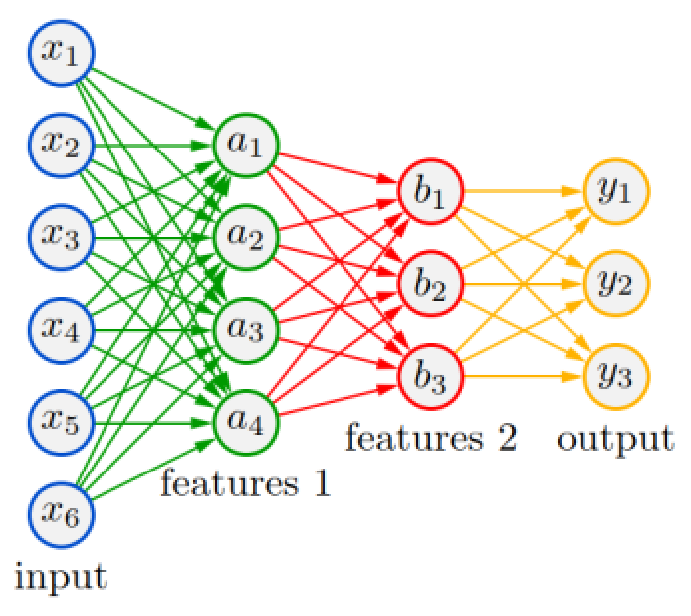
\includegraphics[width=0.6\columnwidth]{img/NN/autoencoder2}
	\end{center}
	Put everything together and, optionally, fine tune it with backpropagation, but it already should be very close to the optimal value.
\end{itemize}

\newpage

\subsection{Convolutional Neural Networks}
Still deep learning, we still have many layers. The difference with standard MLPs brought by Convolutional Neural Networks CNNs is \textbf{reducing the receptive field}, the \textbf{number of connections} such that \textbf{every neuron is connected to a limited number of input data}; so far everything was fully connected, with CNNs we remove this constraint. Each hidden neuron is connected only to a partial region of the input (previous layer).\\

This allows to have very deep networks, since the number of connections is reduced. The more hidden layers allow for more abstract representations and thus increasing understanding capabilities of the network without increasing too much the number of connections.\\

\textbf{Each neuron} of the first hidden layer is \textbf{connected to a few input neurons}
\begin{center}
	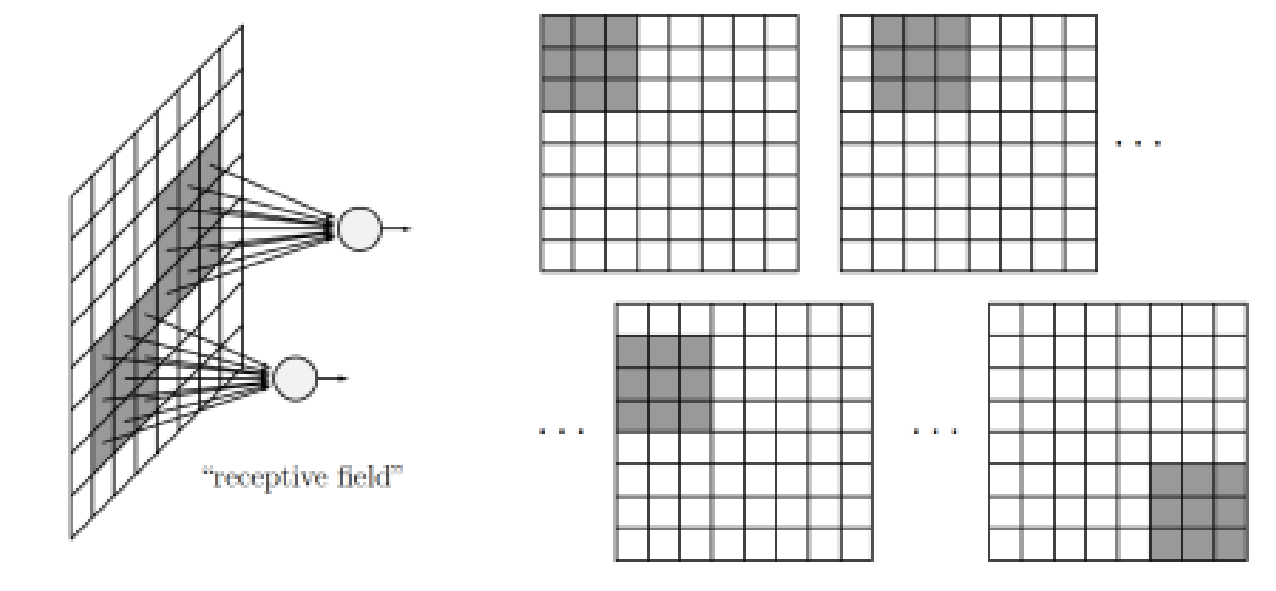
\includegraphics[width=0.7\columnwidth]{img/NN/CNN1}
\end{center}
In this example the neuron is connected to a $3 \times 3$ \textbf{kernel}.\\

The "Convolutional" comes from the fact that the \textbf{connections weights are shared}, all neurons in the same layer have the same weights. Since all the connections are kinda the same it's like sliding a window over an image and doing a \href{https://en.wikipedia.org/wiki/Convolution}{convolution} with that particular kernel. The input field is "moved" step by step over the whole image and doing the equivalent of a convolution.\\

\newpage

There are usually multiple neurons with the same receptive field, to compute multiple convolutions for different weight matrices/features.\\

We're not forced to have always the same kernels across multiple layers, they can be different with different weights.\\
Based on what the weights are each layer will be trained to "look" for different things in the image.\\

Neurons in the successor layer apply \textbf{maximum pooling} over small regions, after the convolution there's a maximum pooling layer, and it will output only the maximum activation of the neurons for each sampled region (kernel). I maintain the obtained results, but I don't know where, pooling \textbf{maintains knowledge} of the features, \textbf{not their location} in the image, but we're not interested in the exact location; if I have to make a classification, at the end of multiple pooling layers I will have a single activation value which will give me my answer. \\
Remove noise, keep knowledge. \textbf{Further layers} allow for \textbf{high-level features}.\\

In a CNN multiple stages of convolution, maximum pooling and ReLUs can be present, building a \textbf{hierarchy of image features}.\\

CNNs are \textbf{translation invariant}: with the way they're built they don't care where an object is (property of convolution) they just find it, the window is sliding, it will get there eventually. The pooling will remove the location from the image.\\

% End NN L9

\newpage

\subsection{Radial Basis Function Networks}
Another topology of NN, Radial Basis Function (RBF) Networks are feed-forward neural networks with a strictly layered structure, with \textbf{always three layers}, one hidden layer in which radial basis functions are employed. Kinda the opposite direction of deep learning.\\

RBF are used as \textbf{activation function in the hidden layer}. An RBF is a function that has its peak at zero and decreases in all other directions.\\

The network \textbf{input function of the output neurons} is the \textbf{weighted sum of their inputs}. From hidden to output neuron there's a "classical" weighted sum.\\

The \textbf{input function of each hidden neuron} is a \textbf{distance} function of the \textbf{input} vector and the \textbf{weight} vector (distance between input and weight). Each hidden neuron has a weight vector and receives the distance between input and weight vectors; it's not a weighted sum. It can be seen as any type of Euclidean distance function: 
\begin{itemize}
	\item $\forall u \in U_{hidden}: \, f_{net}^{(u)} \left(\vec{w}_u, \vec{in}_u \right) = d \left(\vec{w}_u, \vec{in}_u \right)$
	\item $d \left(\vec{x}, \vec{y}\right) = 0 \Leftrightarrow \vec{x} = \vec{y}$
	\item $d \left(\vec{x}, \vec{y}\right) = d \left(\vec{y}, \vec{x}\right)$, Symmetry
	\item $d \left(\vec{x}, \vec{z}\right) \leq d \left(\vec{x}, \vec{y}\right) + d \left(\vec{y}, \vec{z}\right)$, Triangle inequality
\end{itemize}

There can be different families of distances, we'll consider the \textbf{Minkowski Family}, which are distances defined by the formula
$$ d_k \left(\vec{x}, \vec{y}\right) = \left(\sum_{i=1}^n |x_i - y_i|^k \right)^{\frac{1}{k}} $$
With different values of $k$ we have different distances: 
\begin{itemize}
	\item $k = 1:$ Manhattan distance
	\item $k = 2:$ Euclidean distance
	\item $k \rightarrow + \infty:$ Maximum distance
\end{itemize}

\newpage

\begin{center}
	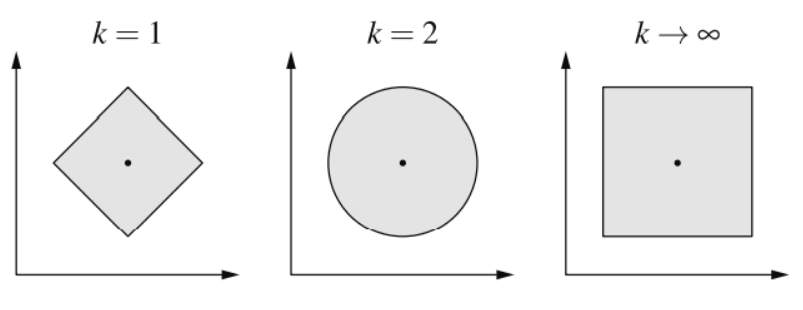
\includegraphics[width=0.7\columnwidth]{img/NN/distances}
\end{center}

The \textbf{activation function} of each \textbf{output neuron} is a \textbf{linear function}, weighted sum that propagates to the output.\\
The \textbf{activation function} of each \textbf{hidden neuron} is a \textbf{radial function}, which decreases monotonically from $0$ to $\infty$
$$ f: \, \mathbb{R}_0^+ \rightarrow [0,1] \; \text{ with } \; f(0) = 1 \; \text{ and } \; \lim_{x \rightarrow \infty} f(x) = 0 $$ 
Basically a bell shape, like a Gaussian.\\
The \textbf{size of the catchment region} is \textbf{defined by the reference radius} $\sigma$, defines the shape and width of the function and thus the area "observed" by the neuron. Some examples of radial functions:
\begin{itemize}
	\item Rectangle function
	$$f_{act} (net, \sigma) = \begin{cases}
		0, & \text{ if } net > \sigma \\
		1, & \text{ otherwise }
	\end{cases} $$
	
	\item Triangle function
	$$f_{act} (net, \sigma) = \begin{cases}
		0, & \text{ if } net > \sigma \\
		1 - \frac{net}{\sigma}, & \text{ otherwise }
	\end{cases} $$
	\begin{center}
		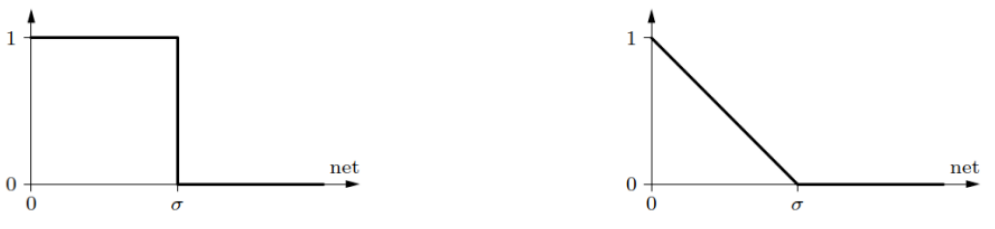
\includegraphics[width=0.95\columnwidth]{img/NN/radial1}
	\end{center}
	
	\newpage
	
	\item Cosine until zero
	$$f_{act} (net, \sigma) = \begin{cases}
		0, & \text{ if } net > 2\sigma \\
		\frac{\cos \left(\frac{\pi}{2 \sigma} net\right) + 1}{2}, & \text{ otherwise }
	\end{cases} $$
	
	\item Gaussian function
	$$f_{act} (net, \sigma) = e^{\frac{net^2}{2 \sigma^2}} $$
	\begin{center}
		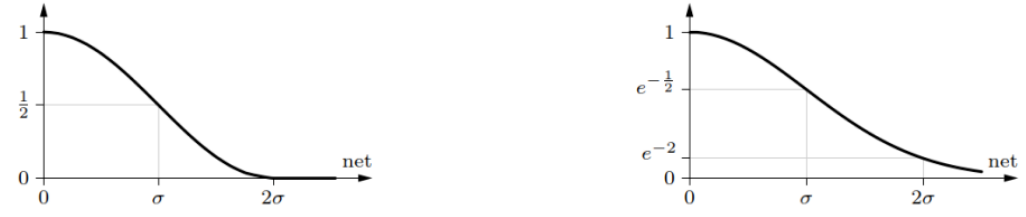
\includegraphics[width=0.95\columnwidth]{img/NN/radial2}
	\end{center}
\end{itemize}

Each neuron can have its own function, maybe just with different $\sigma$, the function is activated based on the distance between weight and input; the weight vector acts as center for the function and the activation is proportional to how far the input is to that radial function. Each neuron has a function centered in a different place. This draws a circle (or equivalent) in the feature space, while an MLP draws a line.\\

\paragraph{Example:} RBF network for the conjunction $x_1 \wedge x_2$. We want to create a circle around the area in which the output is 1:
\begin{center}
	\includegraphics[width=0.8\columnwidth]{img/NN/RBF1}
\end{center}
Another approach could consist in considering the RBF in the opposite way, where the data is outside the circle:
\begin{center}
	\includegraphics[width=0.8\columnwidth]{img/NN/RBF2}
\end{center}

\newpage

\paragraph{Example:} For the bi-implication $x_1 \leftrightarrow x_2$
$$ x_1 \leftrightarrow x_2 \equiv (x_1 \wedge x_2) \vee \neg (x_1 \vee x_2) $$
\begin{center}
	\includegraphics[width=0.75\columnwidth]{img/NN/RBF3}
\end{center}
Here we draw 2 circles around the 2 output that give 1, each of the 2 hidden neurons constitutes a circle with different center.\\

\subsubsection{Function approximation}
MLPs basically \textbf{create a function approximation by a series of steps}. With RBFs we can do the same, but it gives us \textbf{more choices for how to approximate}. A \textbf{step function} can be modeled by an RBF as a \textbf{weighted sum of rectangular functions}, with the same result as MLPs. 
\begin{center}
	\includegraphics[width=0.85\columnwidth]{img/NN/FA1}
\end{center}

\newpage

And the NN would be
\begin{center}
	\includegraphics[width=0.5\columnwidth]{img/NN/FA2}
\end{center}
$$ \sigma = \frac{1}{2} \Delta x = \frac{1}{2} (x_{i+1} - x_i)$$

But we're not limited to this, we could use triangular pulses, considerably \textbf{improving the approximation} (or same approximation with fewer neurons)
\begin{center}
	\includegraphics[width=0.85\columnwidth]{img/NN/FA3}
\end{center}

We can \textbf{use any kind of function}, not only triangular, for example Gaussian functions which would produce "smooth" transitions between our "steps". The weights between input and hidden determine the locations of the Gaussian functions while the weights of the connections from the hidden neurons to the output neuron determine the height/direction (upward or downward) of the Gaussian functions.

% End NN L10, pag 64

\newpage

\subsubsection{Training Radial Basis Function Networks}
We'll consider a case of supervised learning with a \textbf{fixed task} $L_{fixed} = \{l_1, \, ... \, , l_m\}$ with $m$ training patterns $l = \left(\vec{i}^{(l)}, \vec{o}^{(l)}\right)$.\\

Considering a \textbf{simple radial basis function network} which is a partial view of the general structure of a RBFN, where \textbf{each training example is covered by its own radial basis function}. One hidden neuron $v_k$, $k = 1, \, ... \, , m$ for each training pattern
$$ \forall k \in \{1, \, ... \, , m\}: \, \vec{w}_{v_k} = \vec{i}^{(l_k)} $$

The weights of the connections to the hidden neurons are simply initialized with the elements of the input vector of this training example.\\

If the \textbf{activation function} is \textbf{Gaussian}, the radii $\sigma_k$ are \textbf{chosen heuristically}:
$$ \forall k \in \{1, \, ... \, , m\}: \, \sigma_k = \frac{d_{max}}{\sqrt{2m}} $$
$d_{max}$ is the \textbf{maximal distance} between the \textbf{input vectors} of two training patterns
$$ d_{max} = \max_{l_j, l_k \in L_{fixed}} d\left(\vec{l}^{(l_j)}. \vec{l}^{(l_k)}\right)$$
this distance is chosen in a way that doesn't interfere with other patterns. Each radial function should not interfere with other patterns.\\

Having one hidden neuron for each training pattern means that the function is centered around that specific training pattern, the weights are set to the same values as the pattern, so the function will reach the maximum value for that particular training pattern (the distance will be zero); the function is centered around the specific training pattern. \\

\newpage

\paragraph{Initialization:} The connections from hidden to output neurons can be initialized by the formula
$$ \forall u: \, \sum_{k=1}^m w_{uv_m} out_{v_m}^{(l)} - \theta_u = o_u^{(l)} $$

We can analytically solve the problem to find the values of these weights. We know the desired output, threshold and current output, so we know everything besides the \textbf{weights}, which can be \textbf{obtained} by \textbf{multiplying} the \textbf{interconnections weight} by the \textbf{matrix} $\bm{A}$ of the \textbf{hidden layer output}, considering $\theta = 0$:
$$ \bm{A} \cdot \vec{w}_u = \vec{o}_u $$

Where $\vec{o}_u = \left(o_u^{(l_1)}, \, ... \, , o_u^{(l_m)}\right)^T$ is the vector of desired outputs, $\theta_u = 0$ and $\bm{A}$ is the $m \times m$ \textbf{matrix} that has for components the \textbf{various output of the neurons in the hidden layer}:
$$ \bm{A} = \left\{
\begin{array}{c c c c}
	out_{v_1}^{(l_1)} & out_{v_2}^{(l_1)} & \dots & out_{v_m}^{(l_1)} \\
	out_{v_1}^{(l_2)} & out_{v_2}^{(l_2)} & \dots & out_{v_m}^{(l_2)} \\
	\vdots & \vdots & \vdots & \vdots \\
	out_{v_1}^{(l_m)} & out_{v_2}^{(l_m)} & \dots & out_{v_m}^{(l_m)} \\
\end{array}
\right\}$$

Each matrix row contains the outputs of the different neurons for one training example, each column contains the outputs of one hidden neuron for all training examples.\\

Can be \textbf{solved by inverting} $\bm{A}$
$$ \vec{w}_u = \bm{A}^{-1} \vec{o}_u $$

This method guarantees a \textbf{perfect approximation}. This means that is not necessary to train a simple radial basis function network. In general, if we don't want to have a neuron for each pattern, we'll have to select $k$ subsets from the dataset and find, for each subset, a representative that will be associated to a neuron in the hidden layer. \\

\newpage

\paragraph{General Radial Basis Functions:} Not the simple case, we can't have one neuron for each training sample. RBFN usually (always) possess \textbf{fewer neurons} in the hidden layer \textbf{than} there are \textbf{training examples}, otherwise it would not be feasible due to complexity and sometimes not even useful (what if the examples are clustered together?).\\

We need to \textbf{select a subset} of $k$ \textbf{training patterns} as centers
\begin{itemize}
	\item Connection \textbf{weights} for the \textbf{hidden neurons}: \textbf{training patterns} (the chosen ones)
	\item Connection \textbf{weights} for \textbf{output neurons}:
	$$ \bm{A} = \left\{
	\begin{array}{c c c c c}
		1 & out_{v_1}^{(l_1)} & out_{v_2}^{(l_1)} & \dots & out_{v_m}^{(l_1)} \\
		1 & out_{v_1}^{(l_2)} & out_{v_2}^{(l_2)} & \dots & out_{v_m}^{(l_2)} \\
		\vdots & \vdots & \vdots & \vdots & \vdots \\
		1 & out_{v_1}^{(l_m)} & out_{v_2}^{(l_m)} & \dots & out_{v_m}^{(l_m)} \\
	\end{array}
	\right\}$$
	Using the pseudo-inverse matrix since it's over-determined (it's not square, $m$ equations for each output neuron from the training examples but only $k+1$ weights from the $k$ neurons and the $1$ bias value, with $k < m$; more equations than unknowns, more training patterns than weights).
\end{itemize}

How do we \textbf{choose the centers}? How we select the centers can influence the training
\begin{itemize}
	\item \textbf{Random subsets:} select randomly, fast and only radius and output weights need to be determined, but the performance depends on the choice of data points (on which we have no control over)
	\item \textbf{All data points:} like the simple RBFN, only radius and output weights need to be determined and output values can be achieved exactly, but computing the weights can become unfeasible 
	\item \textbf{Clustering:} find the centers of the data with a dedicated algorithm, C-means clustering
\end{itemize}

\newpage

\paragraph{C-means clustering:} Used to find RBFN centers
\begin{enumerate}
	\item Considering a \textbf{number of} $c$ \textbf{clusters} to be found (input)
	
	\item \textbf{Initialize} the cluster centers \textbf{randomly}
	
	\item \textbf{Assign} each \textbf{data point} (the examples) to the \textbf{closest cluster center} (or \textit{centroid})
	
	\item \textbf{Adjust} the \textbf{position} of the \textbf{center} considering the values of the assigned data points (mean vectors of the assigned data points, this is called cluster center update)
	
	\item \textbf{Repeat} the \textbf{step 3 and 4} until clusters do not move anymore (convergence).
\end{enumerate}
The idea is, get $c$ clusters, start with an approximate center and move it one step at a time, it will reach the actual center of the cluster, eventually.\\

Example: with $c=3$ we choose random centers
\begin{center}
	\includegraphics[width=0.65\columnwidth]{img/NN/clustering1}
\end{center}
Then we can use the \textbf{Delaunay Triangulation} of the centers (make triangles out of the centroids, left), which leads to the \textbf{Voronoi Diagram}, by taking the line orthogonal to each one of the three edges (right). This will result in a tessellation of the domain of the function, basically each tassel of the domain is a cluster.
\begin{center}
	\includegraphics[width=0.65\columnwidth]{img/NN/clustering2}
\end{center}

\newpage

After that we can search for the new center of each cluster, where the sum of the distances is minimal, after finding it we can apply again the same partition (Delunay-Voronoi) as before and repeat the process with the new data points added by the new partition.
\begin{center}
	\includegraphics[width=0.9\columnwidth]{img/NN/clustering3}
\end{center}

We can add backpropagation, we can \textbf{train the network}; if we have fewer hidden neurons there are training examples the quality of the RBFN can usually be improved by training. Update rules are analogous to MLPs.\\

We can update the weights from hidden to output neurons, the center coordinates (weights from input to hidden neurons) and the radii of the radial basis functions. We can do this by \textbf{following the backpropagation rules}, using the derivation of the output with respect to the variation of the weight.\\

A \textbf{3 phases RBF} consists of:
\begin{itemize}
	\item Phase 1: find output connection weights with inverse
	\item Phase 2: find RBF centers (e.g. clustering)
	\item Phase 3: error backpropagation
\end{itemize}
An RBFN with good initialization, clustering and backpropagation can obtain good performance.\\

% End of L11

\newpage

\subsection{Learning Vector Quantization}
\textit{What if we don't know the output?} So far we've only considered fixed learning tasks (input/output pairs, supervised learning), which allowed us to describe training as error minimization. Now we'll be considering \textbf{free learning tasks} (unsupervised learning): the data consists \textbf{only} of \textbf{input values}/vectors. The \textbf{objective} is to \textbf{produce similar outputs for similar inputs} (clustering).\\

The concept behind a lot of unsupervised approaches is \textbf{finding clusters} in a given set of data points. The algorithm will work towards finding the given number of clusters and represents them with their center (or a reference vector, same thing).\\

We can still use the Delunay and Voronoi approach to find clusters. But we want to use \textbf{Learning Vector Quantization}, which is a way to \textbf{find a suitable quantization} (many-to-few mapping, often to a finite set) of the \textbf{input space} (e.g. tessellation of a Euclidean space), a way to \textbf{divide in cluster} the input space.\\

Training \textbf{adapts} the \textbf{coordinates of reference} or \textbf{codebook vectors} (centers), each of which \textbf{defines a region in the input space}.\\

Learning vector quantization \textbf{processes the data points one by one} and \textbf{adapts only one reference vector per data point}. The procedure is known as \textbf{competitive learning}: the training patterns (data points) are traversed one by one. For each training pattern, a "competition" is carried out, which is \textbf{won by the output neuron that yields the highest activation for this training pattern} (if distance and activation functions are the same for all output neurons, we may say equivalently: whose reference vector is closest to the training vector). Only this "winner neuron" is adapted. \\

It's still a way to find the centers of the clusters in a way that makes inferring the class of the object possible. There is a learning process called competitive learning, we find the reference vector (center) closest to our input and its position will be updated before going to the next training pattern.

\newpage

\subsubsection{Learning Vector Quantization Networks}
A \textbf{Learning Vector Quantization Network} (LVQ/LVQN) is a \textbf{feed-forward 2-layered neural network}. It can be seen as RBF without the output layer, the hidden layer is used as output, the hidden layer outputs the corresponding activation for each of the neurons and that's the final output. For this reason "hidden" and "output" neurons will be used interchangeably.\\

The \textbf{network input function} for each \textbf{output neuron} is a \textbf{distance function} of the \textbf{input vector and the weight vector}. The definition of the distance is the same. Each neuron in the hidden layer has its own radial function centered in a different place (it might be the same function, but each one has its own weight vector centering it in a different place) whose input is a distance from input to weight vector (since it acts as center of the function).\\

The \textbf{output function} of \textbf{each output neuron} is not a simple function of the activation of the neuron, it \textbf{considers the activation of all output neurons}
$$ f_{out}^{(u)} (act_u) = \left\{
\begin{array}{c c}
	1 & \text{ if } act_u = \max_{v \in U_{out}} act_v \\
	0 & \text{ otherwise }
\end{array}
\right\}$$ 
It's \textbf{winner-takes-all}. \\

Biggest activation will lead to a value of 1, 0 otherwise. We have one neuron winning over all the other, basically we have a connection between all neurons in the output layer such that each of them is able to see what the other neurons are doing (the activation), allowing the confrontation. All outputs will be 0, except one, which will be 1. If more than one unit has the maximal activation, one is selected at random, but if it happens we probably have chosen more cluster than needed.\\

In the LVQN we can use the same radial functions that are use for any RBFN.

\newpage

\paragraph{Learning rules:} We want to learn the position of the reference vector (center of the radial function) of the cluster. For each training pattern we find the closest reference vector (winner neuron) and adapt only that one. Each reference vector is assigned to a class.\\

To \textbf{adjust the weights} we can use (assuming supervised learning):
\begin{itemize}
	\item \textbf{Attraction rule}, when data point and reference vector have the same class (output is of the correct class)
	$$ \vec{r}^{(new)} = \vec{r}^{(old)} + \eta \left(\vec{x} - \vec{r}^{(old)}\right)$$
	We move the reference vector closer to the input point.\\
	
	\item \textbf{Repulsion rule}, when data point and reference vector have different class (output is of the wrong class)
	$$ \vec{r}^{(new)} = \vec{r}^{(old)} - \eta \left(\vec{x} - \vec{r}^{(old)}\right)$$
	Complementary to the last one, the output is of the wrong class, the reference vector has to be moved further away.\\
\end{itemize}

Where $x$ is the input, $r$ is the reference vector and $\eta$ is a learning rate ($0 < \eta < 1$).\\

Representation of the idea:
\begin{center}
	\includegraphics[width=0.9\columnwidth]{img/NN/LVQ1}
\end{center}

\newpage

The adaptation of reference vectors through some epochs (not many, there's still some training to do) can be seen here:
\begin{center}
	\includegraphics[width=0.9\columnwidth]{img/NN/LVQ2}
\end{center}
Online training on the left, batch training on the right.\\

We can see the random initialization of the reference vectors and the average movement (especially in batch training) goes towards the center of the clusters, the centers of the Gaussian functions get weighted towards the right values.\\

\paragraph{Time dependent learning rate:} \textbf{Fixed learning rate} $\eta$ can \textbf{lead to oscillations}, the centers can move without never converging (left image, $\eta(t) = 0.5$). A solution for this can be \textbf{time dependent learning rate}, the parameter $\eta$ gets smaller with time (right image, $\eta(t) = 0.6 \cdot 0.85^t$, starting at $t=0$).
\begin{center}
	\includegraphics[width=0.9\columnwidth]{img/NN/LVQ3}
\end{center}
This way instead of oscillating forever the value of the reference vector converges to the center.\\

\newpage

\paragraph{Update rule for classified data:} We can update not only the reference vector that is closest to the data point, but \textbf{update the two closest reference vectors}, provided that they are of two different classes. This enables to apply \textbf{attraction and repulsion rule} at the \textbf{same time}.\\

It's a way to use the most significant training patterns to update the network more. If the two closest centers to a pattern are from different classes it means that the pattern is on the boundary of said classes, and thus meaningful. We move the correct class closer and the wrong one further away.\\

\paragraph{Window Rule:} Standard learning vector quantization may \textbf{drive the reference vectors further and further apart}. The drawback of the repulsion rule is that it might push the centers far away. The \textbf{window rule} is a way to reduce this problem, the \textbf{update} happens \textbf{only if the data point $\vec{x}$ is close to the classification boundary}, the point must lie close to the (hyper-)surface that separates the regions in which different classes are predicted. The formula is:

$$ \min\left(\frac{d(\vec{x}, \vec{r}_j)}{d(\vec{x}, \vec{r}_k)}, \frac{d(\vec{x}, \vec{r}_k)}{d(\vec{x}, \vec{r}_j)}\right) > \theta \; \text{ where } \; \theta = \frac{1 - \xi}{1 + \xi} $$

Where $\xi$ is a parameter specified by a user, and it describes the "width" of the window around the classification boundary. Note that $\vec{r}_j$ and $\vec{r}_k$ must be of two different classes.\\

This rule prevents a divergence of the reference vectors because the \textbf{adaptation} caused by a data point \textbf{stops as soon as the classification border is far enough away}.\\

\paragraph{Soft-Learning vector quantization:} Instead of the winner-takes-all approach, we can have a \textbf{soft assignment}, all the neurons will output \textit{something}, not zero, essentially giving a probability of being correct to each classification. The assumption is that the given data was samples from a mixture of normal distributions. The adaptation is done with the help of \textbf{gradient descent}, \textbf{maximizing} an objective function that describes the \textbf{probability} that a \textbf{data point is correctly classified}.

% End of L12

\newpage

\subsection{Self-Organizing Maps}
\textbf{Self organizing maps} (SOM), sometimes also called \textbf{Kohonen feature map} (by the name of their inventor), are a feed forward neural network with 2 layers, similar to the Vector Quantization Learning networks, \textbf{with local connections only among neighboring hidden/output neurons}. We're organizing the centers of neighboring radial functions to be close to each other. An LVQ with centers organized in some way. \\

The network \textbf{input function} of each input neuron is a \textbf{distance function} of \textbf{input} and \textbf{weight} vector. The \textbf{activation function} of each output neuron is a \textbf{radial function}. \\

The output function of each output neuron is the identity, and the output is often discretized according to the winner-takes-all principle. \\

On the \textbf{output neurons} a \textbf{neighborhood relationship is defined}. This means that the centers of the radial function are connected together, neighboring neurons will have centers which are close together. This leads to a (usually two-dimensional) \textbf{grid of neurons}. For example:
\begin{center}
	\includegraphics[width=0.85\columnwidth]{img/NN/SOM1}
\end{center}

The radial functions are placed in a two-dimensional space. Each neuron is connected to its nearest neighbor and has a region assigned to it. The \textbf{neighborhood relationship} of the output neurons is usually \textbf{defined} by \textbf{arranging these neurons into a} (usually two-dimensional) \textbf{grid}. \textbf{Reference vectors close to each other} in the input space belong to \textbf{neurons} that have a \textbf{small distance from each other}.\\

\newpage

\paragraph{Topology Preserving Mapping:} The SOM perform a \textbf{meaningful dimensionality reduction}, e.g. we have data in 3 dimensions, and we want to reduce it to 2 (just like the projection of the globe on a map). But we still want to \textbf{preserve the topology} (points near to each other on the globe will be close together on the map), although angles, distances and areas may be distorted. We're not inventing a new map, we're projecting something in a meaningful way, which approximately preserves the position of points.

\begin{center}
	\includegraphics[width=0.9\columnwidth]{img/NN/topology1}
\end{center}

Images of \textbf{points close to each other} in the \textbf{original space} should be \textbf{close to each other} in the \textbf{image space}.\\

With topology preserving maps we can \textbf{map high-dimensional structures} (input space) \textbf{onto low-dimensional spaces} (neuron space/grid).\\

We need to adjust the training to incorporate maintaining the neighboring structure. This works only on \textbf{unsupervised learning/free-learning tasks}, the algorithm should be free to adjust the mapping and the classes by itself. In the training we need to respect the neighborhood, so we need to modify the attraction rule to consider the concept of neighborhood:
$$ \vec{r}_u^{(new)} = \vec{r}_u^{(old)} + \eta(t) \bm{f_{nb} \left(d_{neurons} (u, u_{\ast}), \varrho (t)\right)} (\vec{x} - \vec{r}_u^{(old)}) $$
Where: 
\begin{itemize}
	\item $u_\ast$ is the \textbf{winner neuron} (reference vector closest to the data point)
	\item the \textbf{neighborhood function} $f_{nb}$ is a \textbf{radial function}
	\item \textbf{Learning rate} and \textbf{neighborhood radius} are \textbf{time-dependent}, they both decrease with time
\end{itemize}
More than one neuron is updated, and it's done in a way which considers the distance between the winner neuron and the one to be adapted. All output neurons in a certain radius will be updated, each with a certain strength (strength and distance defined by the neighborhood function).\\

\newpage

The \textbf{learning rate} will \textbf{decrease with time}, as seen before. The \textbf{neighborhood radius} does the same thing, at the start a bigger area around the winner neuron will be updated, as time goes on this area decreases.\\
This avoids oscillations and ensures convergence.\\

\paragraph{Training:} The weight vector of the neuron in the self-organizing map is \textbf{initialized randomly}, the reference vector are placed randomly in the input/data space, using random training examples.\\

The \textbf{training} itself \textbf{consists of}: 
\begin{itemize}
	\item \textbf{Choosing} a \textbf{training sample}/data point
	\item \textbf{Finding} the \textbf{winner neuron} with the distance function in the data space (neuron with the closest reference vector)
	\item Computing the time dependent radius and learning rate and \textbf{adapt the corresponding neighbors} of the winner neuron
\end{itemize}

\vfill

Example MIA

% End NN L13, L14 video is missing

\newpage

\subsection{Hopfield Networks}
The Hopfield Network (HN) is an ANN with a loop in the graph. It's the simplest type of \textbf{recurrent network}, a graph with direct cycles. \textbf{All} the \textbf{neurons} are \textbf{both input and output}. There is \textbf{no hidden layer} of neurons, each neuron is connected to another (except single neuron loops) and the connection weights are distributed symmetrically. \textbf{Each neuron} receives \textbf{input from all other neurons} while \textbf{not being connected to itself}.\\

A \textbf{Hopfield network} is a \textbf{neural network} with a graph $G = (U, C)$ that satisfies the following conditions:
\begin{enumerate}
	\item $U_{hidden} = \emptyset$, $U_{in} = U_{out} = U$,
	\item $C = U \times U - \{(u, u) | u \in U \}$.
\end{enumerate}

The \textbf{connection weights} are \textbf{symmetric} $\forall u, v \in U,$ $u \neq v: w_{uv} = w_{vu}$. The \textbf{network input function} of \textbf{each neuron} $u$ is the \textbf{weighted sum} of the \textbf{outputs of all other neurons}, that is
$$ \forall u \in U: f_{net}^{(u)} (\vec{w}_u, in_{u}) = \vec{w}_u in_u = \sum_{v \in U - \{u\}} w_{uv} out_v $$

The \textbf{activation function} of each neuron $u$ is a \textbf{threshold function}
$$ \forall u \in U: f^{(u)}_{act} (net_u, \theta_u) =
\begin{cases}
	1 & \text{ if } net_u \geq 0 \\
	-1 & \text{ otherwise}
\end{cases}
$$

The \textbf{output function} of each neuron is the \textbf{identity}, that is
$$ \forall u \in U: f_{out}^{(u)} (act_u) = act_u $$

Since the connection weights are symmetric the \textbf{weight matrix} will obviously be \textbf{symmetric}. A Hopfield network with $n$ neurons $u_1, \, ... \, , u_n$ can be described by the $n \times n$ matrix
$$ 
W = \left(
\begin{array}{c c c c}
	0 & w_{u_1u_2} & \dots & w_{u_1u_n}\\
	w_{u_1u_2} & 0 & \dots & w_{u_2u_n} \\
	\vdots & \vdots & & \vdots \\
	w_{u_1u_n} & w_{u_2u_n} & \dots & 0 
\end{array}
\right)
$$

\newpage

\paragraph{Simple Examples:} A network that oscillates if the activations of the two neurons are updated in parallel, but reaches a stable state if the neurons are updated alternatingly
\begin{center}
	\includegraphics[width=0.45\columnwidth]{img/NN/HN1}
\end{center}
The weight matrix is: 
$$ W = \left[
\begin{array}{c c}
	0 & 1 \\
	1 & 0
\end{array}
\right]
$$
There are no loops in a Hopfield network, that is, no neuron receives its own output as input. All feedback loops run through other neurons: a neuron $u$ receives the outputs of all other neurons as its input and all other neurons receive the output of the neuron $u$ as input. \\

A three neuron example and its simplified representation (right):
\begin{center}
	\includegraphics[width=0.8\columnwidth]{img/NN/HN2}
\end{center}
We don't need to explicitly draw input and output arrows since each neuron is both input and output. The weights are symmetric so a single arrow for both sides it's enough.\\

\newpage

In a network with cycles, such as a Hopfield network, the \textbf{behavior depends} also on the \textbf{update order}:
\begin{itemize}
	\item \textbf{Synchronous update:} updating the values at the same time, in parallel. This way the computation can oscillate.\\
	
	\item \textbf{Sequential update:} updating the values asynchronously, one after the other. This always leads to convergence, which stable state is reached depends on which neuron is updated first.\\
\end{itemize}

For the three neuron example, an asynchronous update leads either to the stable state $(1, 1, 1)$ or to the stable state $(-1, -1, -1)$. This can be seen with the \textbf{state graph}. \textbf{Each node} in the graph represents a \textbf{configuration for each neuron}. The $+/-$ \textbf{encodes} the \textbf{neuron activation} (active and inactive respectively)
\begin{center}
	\includegraphics[width=0.6\columnwidth]{img/NN/HN3}
\end{center}
\textbf{Labels} on \textbf{arrows} indicate the \textbf{neurons}, whose \textbf{updates} (activation changes) lead to the corresponding state transitions. \\
States shown in \textbf{gray} are \textbf{stable}, cannot be left again. States shown in \textbf{white} are \textbf{unstable}, may be left again.\\

\newpage

\subsubsection{Convergence Theorem}
The convergence theorem states that, if the \textbf{activations of the neurons} of a Hopfield network are \textbf{updated sequentially} (asynchronously), then a \textbf{stable state is reached} in a \textbf{finite number of steps}.\\
If the \textbf{neurons} are \textbf{traversed} and updated \textbf{cyclically} in an \textbf{arbitrary}, but \textbf{fixed order}, at \textbf{most} $n \cdot 2n$ \textbf{steps} (updates of individual neurons) are needed for reach the convergence, where $n$ is the number of neurons of the HN.\\

We can prove this by defining a function that maps every state of a Hopfield network to a real-valued number, which is reduced with every state transition or at least stays the same. This function is commonly called the \textbf{energy function} of the Hopfield network.\\

So, the system can only evolve \textbf{from} one \textbf{state with higher energy} to \textbf{another with lower energy}. A \textbf{stable state} will be a \textbf{local minimum} of the energy function.\\

If in a traversal of all $n$ neurons there are \textbf{no activation changes}: a \textbf{stable state} has been reached.\\
If in a traversal of all $n$ neurons \textbf{at least one activation changes}: the \textbf{previous state cannot be reached again} since updates can't go back to states with higher energy.\\

\newpage

\subsubsection{Associative Memory}
Hopfield networks are very well suited to implement so-called \textbf{associative memory}, that is, a kind of memory that is addressed by its contents. If a pattern is presented to an associative memory, the \textbf{memory returns} whether this \textbf{pattern coincides with one of the stored patterns}. This coincidence need not be exact, it may also return a stored pattern that is as similar as possible to the presented pattern, this way "noisy" patterns can be recognized.\\

The associative memory works by \textbf{exploiting the stable states} of HN. If we determine the \textbf{weights and the thresholds} of a HN in such a way that the \textbf{patterns to store are exactly the stable states}, the normal update procedure of a Hopfield network finds for any input pattern a similar stored pattern.\\

\textbf{Hebbian learning rule}:
\begin{enumerate}
	\item Store one pattern $p$:
	\begin{itemize}
		\item find weights so that pattern is a stable state
		\item $ W = pp^T - E $
		\item $ w_{uv} = \begin{cases}
			0 & u = v \\
			1 & u \neq v, \; act_u^{(p)} = act_v^{(p)} \\
			-1 & \text{ otherwise}
		\end{cases}$
	\end{itemize}
	\nn
	
	\item Storing several patterns
	\begin{itemize}
		\item Compute $W_i$ for each pattern $p_i$
		\item $W = \sum_i W_i$
	\end{itemize}
\end{enumerate}

\newpage

\subsubsection{Solving Optimization Problems}
We can exploit a \textbf{minimization of the energy function} to \textbf{solve optimization problems}, since a Hopfield network reaches a (local) minimum of said function in every stable state.\\

We need to:
\begin{itemize}
	\item Transform \textbf{function to optimize} into a \textbf{function to minimize}.\\
	
	\item Transform \textbf{function} into the \textbf{form of an energy function} of a Hopfield network.\\
	
	\item \textbf{Read} the \textbf{weights and threshold} values \textbf{from} the \textbf{energy function}.\\
	
	\item \textbf{Construct} the corresponding Hopfield network.\\
	
	\item \textbf{Initialize Hopfield network randomly} and \textbf{update until convergence}.\\
	
	\item Read \textbf{solution} from the \textbf{stable state reached}.\\
	
	\item \textbf{Repeat} several times and \textbf{use best solution} found.\\
	
\end{itemize}

The solution found may not be the global optimum since it's just a local minimum.\\

Also, the asynchronous updates limit the kind of changes that the HN can perform, since a change may violate a constraint and increase total energy but multiple changes together may result in a lower energy state.\\

The procedure may get stuck in a local optima, similarly to what happens with many other optimization methods (e.g. gradient descent, hill climbing, alternating optimization).\\

\newpage

\subsubsection{Simulated Annealing}
This is a possible approach to solve the problems given by getting stuck in a local minimum of the energy function.\\

The idea of simulated annealing is to \textbf{start} with a \textbf{randomly generated candidate solution} of the optimization problem and to \textbf{evaluate it}. In every later step, the current \textbf{candidate solution is modified} (slightly) and \textbf{re-evaluated}. \textbf{If} the \textbf{new solution is better} than the old, it is \textbf{accepted and replaces} the old solution. However, \textbf{if it is worse}, it is \textbf{accepted} only \textbf{with a certain probability} that depends on \textbf{how much worse} the new solution is. In addition, this \textbf{probability is reduced over time}. Furthermore, the best solution found so far is usually recorded in parallel.\\

It's an \textbf{extension of gradient descent} that tries to \textbf{avoid getting stuck}, the transition from higher to lower local minimums should be more probable than the opposite.\\

There is still \textit{no guarantee that the global optimum will be found}.\\

\textbf{Algorithm} for a Hopfield network:
\begin{itemize}
	\item All \textbf{neuron activations} are \textbf{initialized randomly}.\\
	
	\item The \textbf{neurons} of the Hopfield network are \textbf{traversed repeatedly} (for example, in some random order).\\
	
	\item For \textbf{each neuron}, it is determined whether an \textbf{activation change} leads to a \textbf{reduction} of the network energy or not.\\
	
	\item An \textbf{activation change that reduces} the network energy is \textbf{always accepted} (in the normal update process, only such changes occur).\\
	
	\item However, \textbf{if} an \textbf{activation change increases} the network \textbf{energy}, it is \textbf{accepted with a certain probability}.\\
\end{itemize}

% End L14 (I think)

\newpage

\subsection{Boltzmann Machines}
An extension to the idea of Hopfield networks, instead of modeling a single pattern, \textbf{Boltzmann machines} want to \textbf{model a probability distribution}. The network is constructed with and wants to encode a probability distribution of the data over the whole input space, we want to understand how the data is structured and its significance. A standard Boltzmann machine differs from a Hopfield network mainly in how the states of the neurons are updated. \\

It's possible to define an \textbf{energy function} that assigns a numeric \textbf{value} (an energy) \textbf{to each state} of the network (as seen in HN). With the help of this function a \textbf{probability distribution over the states} of the network is defined based on the \textbf{Boltzmann distribution}:
$$ P(\vec{s}) = \frac{1}{c} e^{-\frac{E(\vec{s})}{kT}} $$
Where: 
\begin{itemize}
	\item $\vec{s}$ describes the (discrete) \textbf{state of the system}
	\item $c$ is a normalization constant
	\item $E$ is the function that yields the \textbf{energy of a state} $\vec{s}$
	\item $T$ is the thermodynamic temperature of the system 
	\item $k$ is Boltzmann's constant ($k \approx 1.38 \cdot 10^{-23} J/K$)
\end{itemize}

The state of the machine $\vec{s}$ consists of the \textbf{vector} $\vec{act}$ of the \textbf{neuron activations}. The energy function of a Boltzmann machine 
$$ E(\vec{act}) = - \frac{1}{2} \vec{act}^\top W \vec{act} + \vec{\theta}^\top \vec{act} $$
where $W$ is the matrix of connection weights and $\vec{\theta}$ the vector of threshold values. The energy function depends on both the state (outputs) and configuration of the network.\\

\newpage

The \textbf{energy change} resulting from the \textbf{change of a single neuron} $u$:
$$ \Delta E_u = E_{act_u = 1} - E_{act_u = 0} = \sum_{v \in U - \{u\}} w_{uv} act_v - \theta_u = net_u - \theta_u $$

The energy difference/change is closely \textbf{related} to the \textbf{network input}.\\

The \textbf{probability} of a \textbf{neuron being active} is a \textbf{logistic function} of the (scaled) \textbf{energy difference} between its \textbf{active} and \textbf{inactive state}:
$$ P(act_u = 1) = \frac{1}{1 + e^{- \frac{\Delta E_u}{kT}}} $$

\paragraph{Update procedure:} The update step is:
\begin{itemize}
	\item A \textbf{neuron} $u$ is \textbf{chosen} (randomly)
	\item The \textbf{energy difference} $\Delta E_u$ and then the \textbf{probability} of the neuron \textbf{having activation 1} are \textbf{computed}
	\item The \textbf{neuron} is \textbf{set to activation 1} with this \textbf{probability} (and to 0 with the complement of said probability)
\end{itemize}

This update is \textbf{repeated many times} for randomly chosen neurons. There is no update for weights or threshold, we're talking about an already trained Boltzmann machine.\\

\textbf{Simulated annealing} is carried out by slowly lowering the temperature $T$. \\

This is a \textbf{Markov-Chain Monte Carlo (MCMC)} procedure.\\

After enough steps, the \textbf{probability} that the network is in a \textbf{specific activation state} depends only on the \textbf{energy of that state}, it's \textit{independent of the initial activation state} the process started with. This final situation is also referred to as \textbf{thermal equilibrium}.\\

\newpage

\subsubsection{Training}
The \textbf{probability distribution} represented by a Boltzmann machine via its energy function can be \textbf{adapted to a given sample of data points}.\\

Boltzmann machine can represent a probability distribution \textbf{only if the points in the data set are compatible with a Boltzmann distribution}. In order to mitigate this restriction, the neurons of a Boltzmann machine are divided into \textbf{visible} neurons, which \textbf{receive the data points} as input, and \textbf{hidden} neurons, the \textbf{activations} of which are \textbf{not fixed by the data points} and thus allow for a more flexible adaptation to the sample data. This is the first deviation from the structure of Hopfield networks.\\

The objective of the training is to \textbf{adapt weight and threshold values} in such a way that the true \textbf{distribution} underlying a given \textbf{data sample} is \textbf{approximated well} by the probability distribution represented by the Boltzmann machine on its visible neurons.\\

The approach is to \textbf{measure the difference between two probability distributions} and use \textbf{gradient descent} to \textbf{minimize} said difference. Start from random values and, using gradient descent, minimize the difference between the distribution created and the data given.\\

A commonly used measure of difference is the \textbf{Kullback-Leiber information divergence}
$$ KL(p_1, p_2) = \sum_{\omega \in \Omega} p_1 (\omega) \ln \frac{p_1(\omega)}{p_2 (\omega)} $$
Where $p_1$ refers to the data sample and $p_2$ refers to the visible neurons of the Boltzmann machine. It's a \textbf{measure of divergence} between \textbf{two probability distributions}, in our case it becomes like a loss function.\\

\newpage

\textbf{Each training step} there are \textbf{two phases}:
\begin{itemize}
	\item \textbf{Positive phase}: the visible neurons are fixed to a data point chosen randomly, and the hidden neurons are updated until thermal equilibrium is reached.\\
	
	\item \textbf{Negative phase}: all units are updated until thermal equilibrium is reached
\end{itemize}

\paragraph{Update rule:} The update is performed according to the following two equations
$$ \Delta w_{uv} = \frac{1}{\eta} \left(p_{uv}^+ - p_{uv}^-\right) \;\; \text{ and } \;\; \Delta \theta_u = - \frac{1}{\eta} \left(p_u^+ - p_u^-\right) $$
Where $p_u$ indicates the probability that neuron $u$ is active, $p_{uv}$ indicates the probability that neurons $u$ and $v$ are both active simultaneously and the $+, -$ as upper indices indicate the phase referred to (positive and negative respectively).\\

All these probabilities are \textbf{estimated} from the \textbf{relative frequency} with which the \textbf{corresponding situation was observed in the respective phase}.\\

Intuitively: if a \textbf{neuron} is \textbf{more often active when a training example is presented} (i.e., visible units are fixed) than when the network is allowed to run freely (i.e., visible units are updated), the \textbf{probability of the neuron being active is too low}, so the threshold should be reduced.\\
Similarly, if \textbf{two neurons are more often active together} when a \textbf{training example is presented} than when the network is allowed to run freely, the \textbf{connection weight between them should be increased}, so that they become more likely to be active together. \\

This training procedure is \textbf{impractical unless the networks are very small}. The larger the network the more update steps are needed to obtain sufficiently reliable statistics for the neuron activation used in the update formulas. The complexity grows too quickly with the number of neurons.\\

\newpage

\subsubsection{Restricted Boltzmann Machines}
It's a solution to \textbf{limit complexity} with respect to the number of neurons and allow for \textbf{efficient training}.\\

In a Restricted Boltzmann machine (RBM) we have a \textbf{bipartite graph} instead of a fully connected one. The connections only go from neurons in the visible layer to neurons in the hidden layer (no connections among the same group).

\begin{center}
	\includegraphics[width=0.65\linewidth]{img/NN/RBM1}
\end{center}

In an RBM \textbf{all input neurons are also output neurons} and vice versa. There are hidden neurons, which are different from input and output neurons. Each input/output neuron receives input from all hidden neurons and vice versa.\\

Due to the \textbf{lack of connections} within visible and hidden units \textbf{training} can proceed by \textbf{repeating three steps}: 
\begin{itemize}
	\item \textbf{First step}: \textbf{visible units are fixed} to a randomly chosen data sample $\vec{x}$ and \textbf{hidden units are updated} one and in parallel $\vec{y}$, retrieving the \textbf{positive gradient} for the weight matrix $xy^T$.\\
	
	\item \textbf{Second step}: \textbf{hidden neurons are fixed} to the vector $\vec{y}$, \textbf{visible units are updated} one and in parallel to the "reconstruction" $\vec{x}^\ast$. Then \textbf{hidden neurons are updated once more}, $\vec{y}^\ast$, and the \textbf{negative gradient} is obtained $\vec{x}^\ast \vec{y}^{\ast T}$.\\
	
	\item \textbf{Third step}: \textbf{connection weights are updated} with the difference of positive and negative gradient
	$$ \Delta w_{uv} = \eta \left( \vec{x}_u \vec{y}_u^T - \vec{x}^\ast_u \vec{y}^{\ast T}_u \right)$$
\end{itemize}

The RBM have also been used to build deep networks similar to stacked autoencoders for the MLP.\\

%End NN L15

\subsection{Recurrent Networks}
Recurrent networks (RNN) are NN with fewer limitations than the ones seen until now, we want to remove limitations such as no loops on the same neuron, no cycles, only allowing connections between different layers, ecc. We're \textbf{lifting all restrictions}, such as the ones seen for Hopfield networks and Boltzmann machines, and considering \textbf{recurrent networks without any constraints}.\\

The \textbf{output} is generated when \textbf{stability is reached}.\\

The \textbf{configuration} can be
\begin{itemize}
	\item \textbf{by construction} if the structure of the computation is known
	\item \textbf{by extending the error backpropagation algorithm in time} to deal with recursion to output stability for each input pattern
\end{itemize}

RNN can be used to represent differential equations: 
$$ x^{(n)} = f(t, x, x', x'', \, \dots \, , x^{(n-1)}) $$
which is equivalent to a system of differential equations
$$ 
\begin{cases}
	x' = y_1 \\
	y_1' = y_2 \\
	\dots \\
	y_{n-1}' = y_{n-1}\\
	y_{n-1}' = f(t, x, y_1, y_2, \, ... \, , y_{n-1})
\end{cases}
$$
And the recursive representation
\begin{flalign*}
	x(t_i) = & \; x(t_{i-1}) + \Delta t y_1(t_{i-1}) \\
	y_1 (t_i) = & \; y_1 (t_{i-1}) + \Delta t y_2 (t_{i-1}) \\
	\dots & \\
	y_{i-2} (t_i) = & \; y_{i-2} (t_{i-1}) + \Delta t y_{i-3} (t_{i-1}) \\
	y_{i-1} (t_i) = & \; y_{i-1} (t_{i-1}) + f(t_{i-1}, x(t_{i-1}), y_1 (t_{i-1}), \, \dots \, , y_{n-1} (t_{i-1}))
\end{flalign*}
We can represent differential equation using RNN (or vice versa).\\

\newpage

\begin{center}
	\includegraphics[width=0.4\columnwidth]{img/NN/RN1}
\end{center}
The output of the network can be reconstructed by \textbf{considering the output in the previous instant} of time. We can use the derivative of the function at the previous time slice for computing the following value. This allows to transform the equation into an RNN, creating for each variable a node inside the graph and associating to the connections the value of the differential (like in the image).\\

\paragraph{Vectorial Neural Networks:} Recurrent networks can be composed by \textbf{multiple recurrent sub-networks}. It can be used to compute vectorial differential equations (systems with more than one function).

\paragraph{Error backpropagation in time:}  The backpropagation is not directly applicable since \textbf{loops propagate errors in a cyclic manner}. Recurrent networks must be \textbf{unfolded in time} between two training patterns, replicating the structure of the network so that it "simulates an MLP", the loops must be unfolded in a linear/spatial way. We put all neurons in each time slice one after the other and compute the average update (since they're the same connection). The \textbf{backpropagation} is \textbf{computed on the unfolded network} and the \textbf{adjustments of the same weight} are \textbf{combined} to generate the value for the RNN.\\

\newpage

%End NN L16

%End of NN (finalmente)
	
	%%%%%%%%%%%%%%%%%%%%%%%%%%%%%%%%
	% Domande sulla seconda parte:
	% X	Fuzzy Set
	% X	Fuzzy Controller
	% X	Fuzzy Data Analysis
	% X	Neuro-Fuzzy Systems
	%%%%%%%%%%%%%%%%%%%%%%%%%%%%%%%%
	
	\section{Fuzzy Systems}

\subsection{Introduction to fuzzy logic}

What's the \textbf{motivation} behind the use of \textbf{fuzzy logic}? Humans use imprecise linguistic terms and make complex reasoning based on that terms, classical mathematics cannot manage these terms. To use these terms with computer we have fuzzy logic.\\

\subsubsection{Imprecision and Uncertainty}

Any \textbf{notion} is said to be \textbf{imprecise} when its meaning is not fixed, something more than \textit{true} or \textit{false}, the value can be in between, there's a \textbf{gradualness}, also called \textbf{fuzziness}.\\

A \textbf{proposition} is \textbf{imprecise} if it contains \textbf{gradual predicates}, propositions true to a certain degree.\\

Sorites \textbf{paradox}: if a sand dune is small, adding one grain of sand to it leaves it small, a sand dune with a single grain is small, hence all sand dunes are small. What's the threshold for a sand dune?\\
Formulation:
\begin{itemize}
	\item Statement $A(n):$ "$n$ grains of sand are a sand dune"
	\item Let $d_n = T(A(n))$ denote the \textbf{degree of acceptance} for $A(n)$
	\item Then $0 = d_0 \leq d_1 \leq \, \dots \, \leq d_n \leq \, \dots \, \leq 1$ can be seen as \textbf{truth values of a many-valued logic} 
\end{itemize}
There's no definite threshold, there must be different degrees (e.g. the difference between "slow" and "fast" is not 1km/h).\\

Fuzzy set theory \textbf{does not assume any threshold} (no discrete thresholds at least).\\

\newpage

\paragraph{Difference between imprecision and uncertainty:} They're not the same: 
\begin{itemize}
	\item \textbf{Imprecision} does not refer to a probability, it neglects details 
	\item \textbf{Uncertainty} refers to a possibility/probability of something we don't know, it will assume that value with a certain probability
\end{itemize}

\textit{"This car is rather old"}, imprecision, we can't evaluate the numerical feature of "being old".\\
\textit{"This car was probably made in Germany"}, uncertainty, a car is either made in Germany or not, but we don't know which one.\\

\subsubsection{Principle of Incompatibility}
As the \textbf{complexity of a system increases}, our ability to make \textbf{precise} yet \textbf{significant statements} about its behavior \textbf{diminishes}. Until a threshold is reached beyond which \textbf{precision and significance} (or relevance) become almost \textbf{mutually exclusive} characteristics.\\

Fuzzy sets and fuzzy logic are used as a mechanism for \textbf{abstraction of unnecessary or too complex details}.\\

Something to \textbf{bridge the gap} from natural language to automation. Based on context, we can define some kind of threshold for the values needed.\\

Some applications: 
\begin{itemize}
	\item Control engineering 
	\item Approximate reasoning
	\item Data analysis 
	\item Image analysis
\end{itemize}
Advantages: 
\begin{itemize}
	\item Use of imprecise or uncertain information
	\item Use of expert knowledge 
	\item Robust nonlinear control 
	\item Time to market 
	\item Marketing aspects 
\end{itemize}

\newpage

\subsection{Fuzzy Sets}

A \textbf{fuzzy set} is a set of elements with a \textbf{continuum of membership grades}.\\

A fuzzy set $\mu$ of a set $X$ (the universe) is a \textbf{mapping}: 
$$ \mu : X \mapsto [0,1] $$
which assigns to each element $x \in X$ a \textbf{degree of membership} $\mu(x)$ to the fuzzy set $\mu$ itself.\\

$\mu_M (u) = 1$ represents \textbf{full membership} in $M$, while $\mu_M (u) = 0$ expresses \textbf{absolute non-membership} in $M$.\\
Membership degrees $0 < \mu_M < 1$ represent \textbf{partial membership}.\\

"Normal" sets can be viewed as a special case of fuzzy sets where only full membership and absolute non-membership are allowed (crisp sets or Boolean sets).\\

\newpage

\subsubsection{Membership function}

A \textbf{membership function} attached to a given linguistic description \textbf{depends on the context}. E.g., a "young retired person" has a different meaning than "young student".\\

Membership degrees are \textbf{fixed only by convention}. The unit interval as range of membership is arbitrary, could be anything, feels natural to use real numbers.\\

Fuzzy sets offer a \textbf{natural interface} between \textbf{linguistic} and \textbf{numerical} representations.\\

\textbf{Example}: representing "young" in "a young person"
\begin{center}
	\includegraphics[width=0.5\columnwidth]{img/FS/young1}
\end{center}
A person is defined for sure "young" if he has an age of 20 or younger, and is for sure "not young" if over 40, everything in between has a varying degree of "youngness".\\

It doesn't have to be a linear function, other imprecise predicates could be modeled as other functions, such as a sigmoid.\\

Terms like "around" are modeled using different shapes (e.g., triangle, trapezoid, Gaussian, sigmoid, etc.). "Around 2" could be 1.8 or 2.3, it probably won't be 3 and it surely isn't 5.\\

\newpage

\subsubsection{Linguistic variables and linguistic values}

\textbf{Linguistic variables} represent \textbf{attributes} in fuzzy systems. They assume linguistic values.\\

\textbf{Linguistic values} usually \textbf{partition} the possible values of the linguistic variables subjectively (based on human intuition). All linguistic values have a \textbf{meaning}, not a precise numerical number.\\

\textbf{Example}: the linguistic variable is \textit{living area of a flat A}, and the values are \textit{tiny, small, medium, large, huge}
\begin{center}
	\includegraphics[width=0.9\columnwidth]{img/FS/living1}
\end{center}
Every $x \in A$ has $\mu (x) = [0,1]$ to each value.\\

\newpage

\subsubsection{Semantics of fuzzy sets}

What are we trying to model when we define a fuzzy set?\\

Fuzzy sets are relevant in 3 \textbf{types} of information-driven \textbf{tasks}: 
\begin{enumerate}
	\item Classification and data analysis
	\item Decision-making problems 
	\item Approximate reasoning
\end{enumerate}

These tasks exploit three \textbf{semantics of membership grades}: 
\begin{enumerate}
	\item Similarity 
	\item Preference 
	\item Possibility
\end{enumerate}

\paragraph{Degree of Similarity:} $\mu(u)$ is the degree of \textbf{proximity} of $u$ \textbf{from prototype} elements of $u$. Proximity between pieces of information is modeled. This view is used in: pattern classification, cluster analysis, regression. In fuzzy control similarity degrees are measured between current situation and prototypical ones.\\

\paragraph{Degree of Preference:} $\mu$ represents both a \textbf{set of} (more or less) \textbf{preferred objects} and \textbf{values} of a \textbf{decision variable} $X$, while $\mu (u)$ represents both \textbf{intensity of preference} in favor of object $u$ and \textbf{feasibility of selecting} $u$ as a value of $X$. Fuzzy sets represent criteria or \textbf{flexible constraints}. Used in: fuzzy optimization, decision analysis.\\

\paragraph{Degree of Possibility:} $\mu (u)$ can be viewed as degree of \textbf{possibility} that \textbf{parameter} $X$ has \textbf{value} $u$, given the only information "$X$ is $\mu$". It distinguishes plausible cases from less likely ones. Used in: expert systems, artificial intelligence.\\

\newpage

\subsubsection{Representation of Fuzzy sets}

\paragraph{Definition of a set:} By "set" we mean \textbf{every collection} made into a \textbf{whole} of definite, distinct objects of our intuition or of our thought.\\

Properties: 
\begin{itemize}
	\item $x \neq \{x\}$
	\item If $x \in X$ and $X \notin Y$, then $x \notin Y$
	\item The set of all subsets of $X$ is denoted as $2^X$
	\item $\emptyset$ is the empty set
\end{itemize}

\paragraph{Extension to a Fuzzy set:} A fuzzy set $\mu$ of $X \neq \emptyset$ is a \textbf{function} from the reference set $X$ to the unit interval, i.e., $$\mu: X \mapsto [0,1]$$

$\mathcal{F}(X)$ represents the \textbf{set of all fuzzy sets} of $X$, i.e.
$$ \mathcal{F}(X) := \{\mu | \mu X \mapsto [0,1] \} $$

\paragraph{Vertical Representation:} Fuzzy sets are described by their \textbf{membership function} and assigning \textbf{degree of membership} $\mu (x)$ to each element $x \in X$.\\

\textbf{Example}: linguistic expression "approximately between $b$ and $c$": 
$$ \mu_{a,b,c,d} (x) = \begin{cases}
	\frac{x - a}{b - a} & \text{ if } a \leq x \leq b \\
	1 & \text{ if } b \leq x \leq c \\
	\frac{x - d}{c - d} & \text{ if } c \leq x \leq d \\
	0 & \text{ if } x < a \text{ or } x > d
\end{cases}$$

\newpage

\paragraph{Horizontal Representation:} For all membership degrees belonging to chosen subset of $[0,1]$, human expert lists \textbf{elements of $X$ that fulfill vague concept of fuzzy set with degree} $\geq \alpha$. That is the horizontal representation of fuzzy sets by their \textbf{$\alpha$-cuts}. Definition: let $\mu \in \mathcal{F}(X)$ and $\in [0,1]$ Then the sets
$$ [\mu]_\alpha = \{x \in X | \mu (x) \geq \alpha \} $$
$$ [\mu]_{\underline{\alpha}} = \{x \in X | \mu (x) > \alpha \}$$
are called the $\alpha$-cut and strict $\alpha$-cut of $\mu$.\\

For each value $\alpha$ of the unit interval, we consider the set of elements having a membership degree of at least $\alpha$ to the fuzzy set.\\

\textbf{Example}: let $\mu$ be a triangular function on $\mathbb{R}$
\begin{center}
	\includegraphics[width=0.45\columnwidth]{img/FS/hr1}
\end{center}
The $\alpha$-cut of $\mu$ can be constructed by: 
\begin{enumerate}
	\item Draw a horizontal line parallel to the $x$-axis through point $(0, \alpha)$
	\item project this section onto the $x$-axis
	$$ [\mu]_\alpha = \begin{cases}
		[a + \alpha(m-a), b - \alpha (b-m)] & \text{ if } 0 < \alpha \leq 1 \\
		\mathbb{R} & \text{ otherwise }
	\end{cases}$$
\end{enumerate}
Basically, it identifies the set of input values with a membership degree greater than $\alpha$.\\

\newpage

\textbf{Properties} of $\alpha$-cuts: 
\begin{itemize}
	\item \textbf{Any fuzzy set} can be \textbf{described} by \textbf{specifying its $\alpha$-cuts}. Let $\mu \in \mathcal{F} (X)$, $\alpha \in [0,1]$ and $\beta \in [0,1]$
	$$ [\mu]_0 = X$$
	$$ \alpha < \beta \implies [\mu]_\alpha \supseteq [\mu]_\beta $$
	\nn
	
	\item \textbf{Representation theorem}: let $\mu \in \mathcal{F} (X)$, then 
	$$ [\mu]_0 = \sup_{\alpha \in [0,1]} \left\{\min\left(\alpha, \mathcal{X}_{[\mu]_\alpha} (x)\right) \right\} $$
	$$ \text{where }\; \mathcal{X}_{[\mu]_\alpha} (x) = \begin{cases}
		1 & \text{ if } x \in [\mu]_\alpha \\
		0 & \text{ otherwise }
	\end{cases}$$
	Fuzzy sets can be obtained as upper envelope of its $\alpha$-cuts, simply draw $\alpha$-cuts parallel to horizontal axis in height of $\alpha$.\\
	In applications, it is recommended to select finite subset $L \subseteq [0,1]$ of relevant degrees of membership. They must be semantically distinguishable, fix level of fuzzy sets to characterize only for these levels.\\
\end{itemize}

This \textbf{representation} of fuzzy sets is \textbf{used in computers}. For example, suppose $X = [0, 15]$, an expert choose $L = \{0, 0.25, 0.5, 0.75, 1\}$ and $\alpha$-cuts:
\begin{itemize}
	\item $A_0 = [0,15]$
	\item $A_{0.25} = [3,15]$
	\item $A_{0.5} = [4,6] \cup [7,15]$
	\item $A_{0.75} = [4.5,5.5] \cup [7, 15]$
	\item $A_{} = \{5\} \cup [7,15]$
\end{itemize}
\begin{center}
	\includegraphics[width=0.55\columnwidth]{img/FS/hr2}
\end{center}

\newpage

We can see that $\mu_A$ is obtained as upper enveloper of the family $A$ of sets
\begin{center}
	\includegraphics[width=0.55\columnwidth]{img/FS/hr3}
\end{center}
As stated before, this representation is \textbf{easier to process in computers} (it's basically a discrete quantization). Also, the domain of the $x$-axis is usually discretized as well.\\

Discretize the degrees of membership and obtain an approximation of the original fuzzy set. Depending on the considered problem, it must be chosen how fine the discretization should be, there are no general rules.\\
The fuzzy sets are usually determined heuristically or can only be specified roughly.\\

Fuzzy sets are usually stored inside a computer as a chain of linear lists, for each $\alpha$-level, $\alpha \neq 0$.
\begin{center}
	\includegraphics[width=0.7\columnwidth]{img/FS/hr4}
\end{center}
A finite union of closed intervals is stored by their bounds.\\

This data structure is appropriate for arithmetic operators.\\

\newpage

\subsubsection{Support, Core and Height}

\paragraph{Support:} The \textbf{support} $S(\mu)$ of a fuzzy set $\mu \in \mathcal{F}(X)$ is the crisp \textbf{set} that contains \textbf{all elements} of $X$ that have \textbf{nonzero membership} 
$$ S(\mu) = [\mu]_{\underline{0}} = \{x \in X | \mu (x) > 0 \} $$
Basically, the area of the fuzzy set for which the degree of membership is more than zero.\\ \nn

\paragraph{Core:} The \textbf{core} $C(\mu)$ of a fuzzy set $\mu \in \mathcal{F} (X)$ is the crisp \textbf{set} that contains \textbf{all elements} of $X$ that have \textbf{membership of one}
$$ C(\mu) = [\mu]_1 = \{x \in X | \mu(x) = 1 \} $$
All the elements for which I'm sure the linguistic attribute is applicable.\\ \nn

\paragraph{Height:} The \textbf{height} $h(\mu)$ of a fuzzy set $u \in \mathcal{F} (X)$ is the \textbf{largest membership grade} obtained by any element in that set 
$$ h(\mu) = \sup_{x \in X} \{\mu (x)\} $$
A fuzzy set is called \textbf{normal} iff $h (\mu) = 1$, it is called \textbf{subnormal} iff $h(\mu) < 1$.\\

\newpage

\subsubsection{Convex fuzzy sets}
Let $X$ be a vector space. A fuzzy set $\mu \in \mathcal{F} (X)$ is called \textbf{fuzzy convex} if its $\alpha$-cuts are convex for all $\alpha \in (0,1]$.\\

The \textbf{membership function} of a convex fuzzy set is \textbf{not a convex function}.\\

Classical definition: the membership functions are actually \textbf{concave}.\\

\subsubsection{Fuzzy Numbers}
A fuzzy set $\mu$ is a \textbf{fuzzy number} if and only if $\mu$ is \textbf{normal} and $[\mu]_\alpha$ is \textbf{bounded}, \textbf{close}, and \textbf{convex} $\forall \alpha \in (0, 1]$. For example, the term \textit{approximately} $x_0$ is described by a parameterized class of membership functions.
$$ 
\begin{cases}
	[1, 2] & \text{ if } \alpha \geq 0.5 \\
	[0.5 + \alpha, 2) & \text{ if } 0 > \alpha < 0.5 \\
	\mathbb{R} & \text{ if } \alpha = 0
\end{cases}
$$
\begin{center}
	\includegraphics[width=0.4\columnwidth]{img/FS/numbers1}
\end{center}
Upper semi-continuous functions are often convenient in applications. In many applications the class of the functions and their exact parameters have a limited influence on the results. In other applications more precise membership degrees are needed. \\

\newpage

\subsection{Multi-Valued Logics}

The fuzzy concepts seen before referred to a single variable, but how do I compare/combine multiple variables? We need to define a multi-valued logic.\\

\subsubsection{Usual logic concepts}

\paragraph{Set operators:} They are defined by using \textbf{traditional logics operators}. Let $X$ be the universal set: 
\begin{itemize}
	\item $A \cap B = \{x \in X | x \in A \vee x \in B\}$
	\item $A \cup B = \{x \in X | x \in A \wedge x \in B\}$
	\item $A^c = \{x \in X | x \notin A\} = \{x \in X | \neg (x \in A)\}$
	\item $A \subseteq B$ if and only if $(x \in A) \implies (x \in B)$ for every $x \in X$
\end{itemize}

\paragraph{Classical logic:} Considers value which are either \textit{true} or \textit{false}. Propositional logic handles combination of logical variables. The key idea is to express $n$-ary logic functions with logic primitives. \\

A set of logic primitives is \textbf{complete} if \textit{any logic function} can be composed by a finite number of these primitives, e.g.
$$ \wedge, \vee, \neg, NOR, NAND, | $$

\paragraph{Inference rules:} When a variable represented by a logical formula is \textbf{true} for all possible truth values it is called \textbf{tautology}. Instead, when it is \textbf{false} for all possible truth values it is called \textbf{contradiction}. \\

Various forms of tautologies exist to perform deductive inference, and are called \textbf{inference rules}:
\begin{itemize}[label*=]
	\item $(a \wedge (a \rightarrow b)) \rightarrow b$ (modus ponens)
	\item $(\neg b \wedge (a \rightarrow b)) \rightarrow \neg a$ (modus tollens)
	\item $((a \rightarrow b) \wedge (b \rightarrow c)) \rightarrow (a \rightarrow c)$ (hypothetical syllogism)
\end{itemize}

\paragraph{Boolean algebra:} The propositional logic based on finite set of logic variables is isomorphic to finite set theory. Both of these systems are isomorphic to a finite Boolean algebra. %Definition: a Boolean algebra on a set $B$ is defined as quadruple $\mathcal{B} = (B, +, \cdot , \overline{ })$, where $B$ has at least two elements $0$ and $1$, $+$ and $\cdot$ are binary operators on $B$, and $\overline{ }$ is a unary operator on $B$ for the which the following properties hold:

\newpage

\subsubsection{$n$-valued logics}

2-valued logic can be extended to a 3-valued logic in several ways, for example: 
\begin{center}
	\includegraphics[width=0.95\columnwidth]{img/FS/nlogic}
\end{center}
These examples allow for an indeterminate value $\sfrac{1}{2}$. There is no standard interpretation of the truth degrees.\\

Various \textbf{$n$-valued logics} exists. The idea is to \textbf{uniformly divide} the range $[0,1]$ into $n$ \textbf{truth values}, which can be interpreted as \textbf{degrees of truth}. Definition: the set $T_n$ of truth values of an $n$-valued logic is defined as
$$ T_n = {0 = \frac{0}{n-1}, \frac{1}{n-1}, \frac{2}{n-1}, \, \dots \, , \frac{n-2}{n-1}, \frac{n-1}{n-1} = 1} $$

\paragraph{Primitives in $n$-valued logic:} Generalization of \l{L}ukasiewicz three valued logic. It uses truth values in $T_n$ and defines primitives as follows
$$ \neg a = 1 - a $$
$$ a \wedge b = \min (a,b) $$
$$ a \vee b = \max(a,b) $$
$$ a \rightarrow b = \min(1, 1 + b - a) $$
$$ a \leftrightarrow b = 1 - |a - b| $$

This $n$-valued logic is denoted by $L_n$. The sequence $(L_2, L_3, \, \dots \, , L_{\infty})$ contains the classical two-valued logic $L_2$ and an infinite-valued logic $L_{\infty}$ (rational countable values $T_{\infty}$). The infinite-valued logic $L_1$ is the logic with all real numbers in $[0, 1]$ ($1=$ cardinality of continuum).

\newpage

\subsubsection{Fuzzy set theory}

\textit{What does a fuzzy set represent?} A \textbf{logic with values in the range} $[0,1]$. \\

Consider the \textit{fuzzy proposition} $A$ ("approximately two" in the example) on $\mathbb{R}$, fuzzy logic offers means to construct such imprecise sentences

\begin{center}
	\includegraphics[width=0.6\columnwidth]{img/FS/appr2}
\end{center}

$A$ is \textbf{defined} by a \textbf{membership function} $\mu_A$, i.e., truth values $\forall x \in \mathbb{R}$; let $x \in \mathbb{R}$ be a \textbf{subject/observation}, $\mu_A (x)$ is the \textbf{degree of truth} that $x$ is $A$.\\

\paragraph{Standard fuzzy set operators:} We define the following \textbf{algebraic operators} on $\mathcal{F} (X)$ 
\begin{itemize}
	\item $(\mu \wedge \mu') := \min \{\mu(x), \mu' (x)\}$ \textbf{intersection} (AND)
	\item $(\mu \vee \mu') := \max \{\mu(x), \mu' (x)\}$ \textbf{union} (OR)
	\item $\neg \mu := 1 - \mu (x)$ \textbf{complement} (NOT)
\end{itemize}
$\mu$ is subset of $\mu'$ if and only if $\mu \leq \mu'$.\\

\begin{center}
	\includegraphics[width=0.8\columnwidth]{img/FS/fop1}
\end{center}

\textbf{Theorem:} $\mathcal{F} (X), \wedge, \vee, \neg)$ is a complete distributive lattice but not a Boolean algebra.

\newpage

\paragraph{Fuzzy set complement/negation:} Let $X$ be a given set and $\mu \in \mathcal{F} (X)$. Then the complement $\overline{\mu}$ can be defined pointwise by $\overline{\mu} (x) := \sim (\mu (x))$, where $\sim: [0, 1] \mapsto [0,1]$ satisfies the conditions
$$ \sim (0) = 1 \;\;\;\;\;\;\; \sim (1) = 0 $$
and for $x,y \in [0,1]$, $x \leq y \implies \sim x \geq \sim y$ ($\sim$ is non-increasing).\\

A negation is called \textbf{strict} if it is also strictly decreasing (as above but $<$ instead of $\leq$) and continuous. A strict negation is said to be \textbf{strong} if it is \textbf{involutive} ($\sim \sim x = x$, $\forall x \in [0,1]$), too.\\

\textbf{Families of negation}: 
\begin{itemize}
	\item Standard negation
	$$ \sim x = 1 - x $$
	\item Threshold negation
	$$ \neg_\theta x = \begin{cases}
		1 & \text{ if } x \leq \theta \\
		0 & \text{ otherwise }
	\end{cases}$$
	\item Cosine negation: 
	$$ \sim x = \frac{1}{2} (1 + \cos (\pi x)) $$
	\item Sugeno negation: 
	$$ \sim x = \frac{1 - x}{1 + \lambda x}, \;\;\;\;\; \lambda \succ 1$$
	\item Yager negation
	$$ \sim x = (1 - x^\lambda)^{\frac{1}{\lambda}} $$
\end{itemize}

\begin{center}
	\includegraphics[width=0.95\columnwidth]{img/FS/famneg}
\end{center}

No need to remember everything, just note that there can be \textbf{different types of negation}.\\

\newpage

\paragraph{Fuzzy set intersection and union:} Classical set intersection represents logical conjunction. Classical set union represents logical disjunction. \\

Generalization from $\{0,1\}$ to $[0,1]$: Let $A, B$ be fuzzy subsets of $X$, i.e., $A,B \in \mathcal{F} (X)$. Their intersection and union can be defined pointwise using: 
\begin{itemize}[label*=]
	\item T-norm: $(A \cap B) (x) = \top (A(x), B(x))$ where $\top : [0,1]^2 \mapsto [0,1]$
	\item T-Conorm: $(A \cup B) (x) = \bot (A(x), B(x))$ where $\bot : [0,1]^2 \mapsto [0,1]$
\end{itemize}

$\top$ and $\bot$ are called \textbf{triangular norm} and \textbf{triangular conorm}, they take 2 values and give back \textit{something}. For all values they respect identity law, commutativity, associativity and monotonicity. \\

\paragraph{Minimum and Maximum:} Min is the greatest t-norm and max is the weakest t-conorm
$$ \top_{\min} = \min (x, y) \;\;\;\;\;\; \bot_{\max} (x,y) = \max (x, y)$$
So $\top (x,y) \leq \min (x,y)$ and $\bot (x,y) \geq \max (x,y)$ for ant $\top$ and $\bot$.\\

We can choose other function as t-norm or t-conorm which are less \textit{harsh}, but $\top_{\min}$ and $\bot_{\max}$ can be easily processed numerically and visually.\\

\paragraph{Product and Probabilistic Sum:} We can use other functions such as product and sum: 
$$ \top_{\text{prod}} (x,y) = x \cdot y \;\;\;\;\;\; \bot_{\text{sum}} (x,y) = x + y - x \cdot y $$
The use of product and its dual has nothing to do with probability theory.\\

\vfill 

And there are a bunch of other T-norms and conorms which I won't describe right now, but I will name: \textbf{\l{L}ukasiewicz T-Norm and T-Conorm, Nilpotent minimum and maximum, drastic product and sum}.

\newpage

\textbf{Examples} of fuzzy \textbf{intersections:}
\begin{center}
	\includegraphics[width=0.9\columnwidth]{img/FS/fint}
\end{center}

\textbf{Examples} of fuzzy \textbf{unions:}
\begin{center}
	\includegraphics[width=0.9\columnwidth]{img/FS/funion}
\end{center}

There are different intersection/union areas.\\

\newpage

\subsubsection{Fuzzy Implication}

Regarding the \textbf{implication} (if $x$ belongs to $A$ then it belongs to $B$), there are different ways in which fuzzy implications can be defined.\\

One way of defining $I$ is to use $\forall a,b \in \{0,1\}$
$$ I (a,b) = \neg a \wedge b $$

In fuzzy logic, disjunction and negation are t-conorm and fuzzy complement, respectively, thus $\forall a,b \in [0,1]$:
$$ I(a,b) = \bot (\sim a,b) $$

Another way in classical logic is $\forall a,b \in \{0,1\}$
$$ I (a,b) = \max \{x \in \{0,1\} | a \wedge x \leq b \} $$

In fuzzy logic, conjunction represents t-norm, thus $\forall a,b \in [0,1]$
$$ I(a,b) = \sup \{x \in [0,1] | \top (a,x) \leq b \} $$

Classical definitions are equal, fuzzy extensions are not: law of absorption of negation does not hold in fuzzy logic.\\

\newpage

There are \textbf{different ways of handling implications} in \textbf{fuzzy logic}, depending on how the implication is defined:
\begin{itemize}
	\item \textbf{$S$-Implications:} implications based on $I(a,b) = \bot (\sim a,b)$. The symbol $S$ is often used to denote t-conorms.\\
	
	\item \textbf{$R$-Implications:} implications based on $I(a, b) = \sup \{x \in [0, 1]| \top (a, x) \leq b\}$ are called $R$-implication. The symbol $R$ represents close connection to residuated semigroup (whatever this means).\\
	
	\item \textbf{$QL$-implications:} implications based on $\bot (\sim a, \top(a, b))$ are called $QL$-implications, where $QL$ stands for quantum logic.\\
\end{itemize}

\paragraph{Conclusions:} All $I$ come from generalizations of the classical implication. They collapse to the classical implication when truth values are $0$ or $1$. \\

\textit{Which fuzzy implication should be used for calculating the fuzzy relation $R$?} Since the meaning of $I$ is not unique, we must resolve this question. Meaningful criteria are needed, it depends on the situation. \\

\newpage

%End FS L1, app 103

\newpage

\subsection{Theory of Fuzzy Logic}

\subsubsection{The Extension principle}

How do we \textbf{extend operations} to the concept of \textbf{fuzzy sets}.\\

How do we extend functions \textbf{defined on sets to} functions \textbf{defined on fuzzy sets}?
$$ \text{from } \; \phi : X^n \rightarrow Y \; \text{ to } \; \hat \phi : \mathcal{F} (x)^n \rightarrow \mathcal{F} (Y) $$

Let $\mu \in \mathcal{F} (\mathbb{R})$ be a fuzzy set of the \textit{imprecise concept} "about 2", then the degree of membership $\mu (2.2)$ can be seen as truth value of the statement "2.2 is about equal to 2".\\

Any \textit{triangular norm} (t-norm) $\top$: can represent \textbf{conjunction}.\\
Any \textit{triangular co-norm} (t-conorm) $\bot$: can represent \textbf{disjunction}.\\
However, now only $\top_{\min}$ and $\bot_{\max}$ will be used (conjunction of two statements becomes taking the minimum, maximum for the disjunction).\\

Let $\mathcal{P}$ be a \textbf{set of imprecise statements} that can be combined by the operators "\textit{and}" and "\textit{or}", define the \textbf{function} $truth$:
\begin{itemize}
	\item $truth: \mathcal{P} \rightarrow [0,1]$ assigns truth value truth$(a)$ to every $a \in \mathcal{P}$
	\item $truth(a) = 0$ means $a$ is definitely false
	\item $truth(a) = 1$ means $a$ is definitely true
	\item If $0 < truth(a) < 1$ then only gradual truth of statement $a$ 
\end{itemize}

\textbf{Combination} of \textbf{two statements}: 
\begin{itemize}
	\item $truth (a \aand b) = truth(a \wedge b) = \min\{truth(a), truth(b) \}$
	\item $truth (a \oor b) = truth(a \vee b) = \max\{truth(a), truth(b) \}$
\end{itemize}
The $\top$ and $\bot$ for this case, since there's no boolean logic.\\

Extended for an \textbf{infinite number of statements} $a_i$, $i \in I$:
\begin{itemize}
	\item $truth(\forall i \in I: a_i) = \inf \{truth (a_i) | i \in I \}$
	\item $truth(\exists i \in I: a_i) = \sup \{truth (a_i) | i \in I \}$
\end{itemize}
Respectively, the minimum degree of truth satisfied by all and the maximum degree of at least one statement.\\

\newpage

This concept helps to extend $\phi: X^n \rightarrow Y$ to $\hat \phi : \mathcal{F}(X)^n \rightarrow \mathcal{F}(Y)$
\begin{itemize}[label*=]
	\item Crisp tuple $(x_1, \, \dots \, , x_n)$ is mapped to the crisp value $\phi (x_1, \, \dots \, , x_n)$.\\
	
	\item Imprecise descriptions $(\mu_1 , \, \dots \, , \mu_n)$ of $(x_1, \, \dots \, , x_n)$ are mapped to fuzzy value $\hat \phi (\mu_1, \, \dots \, , \mu_n)$.\\
\end{itemize}

\paragraph{Example:} How to extend the addition? With the sum extended to sets
$$ +: 2^{\mathbb{R}} \times 2^{\mathbb{R}} \rightarrow 2^{\mathbb{R}}, \;\;\;\;\; (A,B) \mapsto A + B $$
$$ = \{y | (\exists a) (\exists b) (y = a + b) \wedge (a \in A) \wedge (b \in B) \} $$
(still a sum, just with elements from the sets).\\

This can be \textbf{extended to fuzzy sets}: 
$$ +: \mathcal{F} (\mathbb{R}) \times \mathcal{F} (\mathbb{R}) \rightarrow \mathcal{F} (\mathbb{R}), \;\;\;\;\; (\mu_1, \mu_2) \mapsto \mu_1 \oplus \mu_2$$

$$ truth (y \in \mu_1 \oplus \mu_2) $$
$$ = truth ((\exists a) (\exists b): (y = a + b) \wedge (a \in \mu_1) \wedge (b \in \mu_2)) $$

Up until now it's the same as before. $\exists$ means taking the $\sup$ (as seen earlier), so:
$$ = \sup_{a,b} \{truth (y = a + b) \wedge truth (a \in \mu_1) \wedge truth (b \in \mu_2)\}$$
$$ = \sup_{a,b: y=a+b} \{\min (\mu_1(a), \mu_2(b))\}$$

The greatest $a$ and $b$ such that $y = a+b$ and we consider the minimum of the fuzzy memberships of said $a$ and $b$.\\

\newpage

\paragraph{In general:} A function $\phi: X^n \rightarrow Y$ can be extended to classic sets $\hat \phi: [2^X]^n \rightarrow 2^Y$ with 
$$ \hat \phi (A_1, \, \dots \, , A_n) = \{y \in Y | \exists (x_1 \, \dots \, , x_n) \in A_1 \times \, \dots \, \times A_n : \phi (x_1, \, \dots \, x_n) = y\} $$

And then we can \textbf{generalize to fuzzy sets}:
$$ \hat \phi: [\mathcal{F} (X)]^n \rightarrow \mathcal{F} (Y) $$
with 
$$ \hat \phi (A_1, \, \dots \, , A_n) = \sup \{ \min \{ \mu_1 (x_1), \, \dots \, , \mu_n (x_n) \} |$$ 
$$| (x_1, \, \dots \, , x_n) \in X^n \wedge \phi (x_1, \, \dots \, , x_n) = y \}$$

Assuming that sup $\emptyset = 0$.\\

The mapping of the fuzzy variable is the greatest values of the tuple belonging to $X^n$ such that the minimum of the fuzzy membership is greatest. \\

The minimum of the fuzzy sets should be the greatest, this is the extension principle.\\

\newpage

\subsubsection{Relevant Fuzzy sets}

We'll give particular relevance to fuzzy sets \textbf{defined on} $\mathbb{R}$, with membership function such as
$$ \mu : \mathbb{R} \rightarrow [0,1] $$

These clearly have a \textit{quantitative meaning} and may essentially characterize the \textbf{states of fuzzy variables}. They play an important role in many applications such as fuzzy control, decision-making, approximate reasoning, etc.\\

\textbf{Some relevant classes} $\mathcal{F} (\mathbb{R})$ (set of fuzzy sets) of fuzzy sets $\mu$ (a single fuzzy set) on $\mathbb{R}$ are defined as: 
\begin{itemize}
	\item \textbf{Normal Fuzzy Set:}
	$$ \mathcal{F}_N (\mathbb{R}) := \left\{\mu \in \mathcal{F} (\mathbb{R}) | \exists x \in \mathbb{R}: \mu (x) = 1 \right\} $$
	There's at least an element inside the fuzzy set equal to 1. The maximum membership has to be assigned to \textit{some value}. These make sense in the case of fuzzy numbers ("about 2" will have membership $=1$ for the value 2).\\
	
	\item \textbf{Upper Semi-continuous Fuzzy Set:}
	$$ \mathcal{F}_C (\mathbb{R}) := \left\{\mu \in \mathcal{F}_N (\mathbb{R}) | \forall \alpha \in (0,1] : [\mu]_\alpha \text{ is compact } \right\} $$
	Can be described by an upper semi-continuous function. Not continuous, but at the discontinuity point it includes the upper point, it's \textit{almost continuous}.\\
	
	\item \textbf{Fuzzy Intervals:}
	$$ \mathcal{F}_I (\mathbb{R}) := \left\{\mu \in \mathcal{F}_N (\mathbb{R}) | \forall a,b,c \in \mathbb{R} : c \in [a,b] \right\}$$
	$$ \implies \mu(c) \geq \min\{\mu(a), \mu(b)\} $$
	Membership drops gradually outside a certain interval. Their core is a classical interval, the edges (support) are a slope towards zero.\\
\end{itemize}

\newpage

\subsubsection{Quantitative Fuzzy Variables}

The concept of a fuzzy number plays a fundamental role in formulating \textbf{quantitative fuzzy variables}. These are variables whose \textbf{states are fuzzy numbers}.\\

When the fuzzy quantities \textbf{represent linguistic concepts}, e.g., very small, medium, large etc., then the fuzzy variables are called \textbf{linguistic variables}. Each linguistic variable is \textbf{defined in terms of base variable} which is a variable in the classical sense, e.g., temperature, pressure, age.\\

Linguistic terms \textbf{representing approximate values} of \textbf{base variable} are \textbf{captured by} appropriate \textbf{fuzzy numbers}.\\

Each linguistic variable is \textbf{defined by a quintuple} $(v, T, X, g, m)$ where:
\begin{itemize}
	\item $v$ is the \textbf{name} of the variable
	\item $T$ is the \textbf{set of linguistic terms} of $v$
	\item $X \subseteq \mathbb{R}$ is the \textbf{base variable}
	\item $g$ is the \textbf{syntactic rule} (grammar) for generating linguistic terms
	\item $m$ is the \textbf{semantic rule} that assigns meaning $m(t)$ to every $t \in T$, i.e., $m: T \rightarrow \mathcal{F} (X)$
\end{itemize}

To deal with linguistic variables we need to consider not only set-theoretic operations but also arithmetic operations on fuzzy numbers (i.e., interval arithmetic; something that has a quantitative meaning, e.g., how do we define the double of a fuzzy value? How do we get statistics?).\\

\vfill 

Examples MIA. \\

\newpage

\subsubsection{Efficient Operations}
How do we define \textbf{arithmetic operations} for \textbf{calculating with} $\fr$? In general operations on fuzzy set are \textbf{more complex}.\\

Using \textbf{extension principle} for sum $\mu \oplus \mu'$, product $\mu \odot \mu'$ and reciprocal value $rec(\mu)$ if arbitrary fuzzy sets $\mu, \mu' \in \fr$
$$ (\mu \oplus \mu') (t) = \sup \{\min \{\mu(x_1), \mu'(x_2)\} | x_1, x_2 \in \mathbb{R}, x_1 + x_2 = t\}$$
$$ (\mu \odot \mu') (t) = \sup \{\min \{\mu(x_1), \mu'(x_2)\} | x_1, x_2 \in \mathbb{R}, x_1 \cdot x_2 = t\}$$
$$ rec (\mu) (t) = \sup \left\{\mu(x) | x \in \mathbb{R} \setminus \{0\}, \frac{1}{x} = t \right\} $$

It's desirable to \textbf{reduce fuzzy arithmetic to ordinary set arithmetic}. Then, we apply elementary operations of interval arithmetic.\\

We have to define the set representation.\\

\paragraph{Definition:} A family $(A_\alpha)_{\alpha \in (0,1)}$ of sets is called \textbf{set representation} of $\mu \in \fnr$ if 
\begin{itemize}
	\item $0 < \alpha < \beta < 1 \implies A_\alpha \subseteq A_\beta \subseteq \mathbb{R}$ and
	\item $\mu (t) = \sup \{ \alpha \in [0,1] | t \in A_\alpha \}$
\end{itemize}
holds where $\sup \emptyset = 0$. If the $\alpha$-cuts represent the fuzzy membership we can do the operation on the fuzzy interval.\\

\paragraph{Theorem:} Let $\mu \in \fnr$. The family $(A_\alpha)_{\alpha \in (0,1)}$ is a set representation of $\mu$ if and only if 
$$ [\mu]_{\underline{\alpha}} = \left\{t \in \mathbb{R} | \mu(t) > \alpha \right\} \subseteq A_\alpha \subseteq \left\{t \in \mathbb{R} | \mu(t) \geq \alpha\right\} = [\mu]_\alpha$$
is valid for all $\alpha \in (0,1)$.\\

Let $\mu_1, \mu_2, \, \dots \, , \mu_n$ be normal fuzzy sets of $\mathbb{R}$ and $\phi: \mathbb{R}^n \rightarrow \mathbb{R}$ be a mapping. The $\alpha$-cut of the mapping is the mapping of the $\alpha$-cut.\\

Used to \textbf{execute arithmetic operations on fuzzy sets efficiently}.\\

\newpage

\subsubsection{Interval Arithmetic}
Determining the set representations of arbitrary combinations of fuzzy sets can be reduced very often to simple \textbf{interval arithmetic}.\\

In general, set representation of $\alpha$-cuts of extensions $\hat{\phi} (\mu_1, \, \dots \, , \mu_n)$ cannot be determined directly from $\alpha$-cuts. It always works only for continuous $\phi$ and fuzzy sets in $\fcr$.\\

\paragraph{Theorem:} Let $\mu_1, \mu_2, \, \dots \, , \mu_n \in \fcr$ and $\phi: \mathbb{R}^n \rightarrow \mathbb{R}$ be a continuous mapping. \\
Then $\forall \alpha \in (0,1]: [\hat \phi (\mu_1, \, \dots \, , \mu_n)]_\alpha = \phi ([\mu_1]_\alpha, \, \dots \, , [\mu_n]_\alpha)$.\\

So, a \textbf{horizontal representation} is \textbf{better} than a \textbf{vertical one}.\\

\textbf{Finding} $\hat{\phi}$ values is \textbf{easier than directly applying the extension principle}.\\

However, all $\alpha$-cuts cannot be stored in a computer, only a finite number can.\\

\newpage

\subsubsection{Fuzzy Relations}

A crisp relation represents presence or absence of association, interaction or interconnection between elements of $\geq$ 2 sets. This concept can be generalized to various degree or strengths of association or interaction between elements.\\

A \textbf{fuzzy relation} generalizes these degrees to membership grades. So, a crisp relation is a restricted case of a fuzzy relation. Something can be in relation to something else with a certain degree of truth.\\

\paragraph{Definition of relation:} A \textbf{relation} among \textbf{crisp sets} $X_1, \, \dots \, , X_n$ is a subset of $X_1 \times \, \dots \, \times X_n$ denoted as $R(X_1, \, \dots \, , X_n)$ (so it's a set, more specifically a subset of the Cartesian product). The basic concepts of sets can also be applied to relations.\\

Each crisp relation can be defined by its \textbf{characteristic function}: 
$$ R(x_1, \, ... \, , x_n) = \begin{cases}
	1, & \text{ if and only if } \; (x_1, \, \dots \, , x_n) \in R \\
	0, & \text{ otherwise}
\end{cases}$$
The fuzzy version has not only 0 and 1, but has different degrees of truth.\\

The membership of $(X_1, \, \dots \, , X_n)$ in $R$ means that the \textbf{elements of} $(X_1, \, \dots \, ,X_n)$ are \textbf{related to each other}.\\

A relation can be written as a set of ordered tuples. Thus $R (X_1, \, \dots \, , X_n)$ represents an $n$-dimensional membership array with elements $r_{i_j}$.\\

\newpage

The characteristic function of a crisp relation can be \textbf{generalized to allow tuples to have degrees of membership}. Similar to the generalization of the characteristic function of a crisp set. \\

A \textbf{fuzzy relation} is a \textbf{fuzzy set defined on tuples} $(x_1, \, \dots \, , x_n)$ that may have \textbf{varying degrees of membership within the relation}. \\
The membership grade indicates the strength of the present relation between elements of the tuple. \\

The fuzzy relation can also be \textbf{represented by an $n$-dimensional membership array}. \\

Basically, a fuzzy relation tells us \textit{how much} of the concept the elements have among each other (while a crisp relation tells us only if they have it or not).\\

\paragraph{Cartesian Product of fuzzy sets:} Let $n \geq 2$ fuzzy sets $A_1, \, \dots \, , A_n$ be defined in the universes of discourse $X_1, \, \dots \, , X_n$, respectively.\\
The Cartesian product of $A_1, \, \dots \, , A_n$ denoted by $A_1 \times \, \dots \, \times A_n$ is a fuzzy relation in the product space $X_1 \times \, \dots \, \times X_n$.\\

It's defined by its membership function 
$$ \mu_{A_1 \times \, \dots \, \times A_n} (x_1 \, , \dots \, , x_n) = \top (\mu_{A_1} (x_1), \, \dots \, , \mu_{A_n} (x_n))$$
whereas $x_i \in X_i$, $1 \leq i \leq n$.\\

Usually $\top$ is the minimum (sometimes also the product).\\

\newpage

\paragraph{Subsequences:} Consider the Cartesian product of all sets in the family
$$ X = \{X_i | i \in \mathbb{N}_n = \{1,2, \, \dots \, , n\} \}$$

for each sequence ($n$-tuple)
$$ x = (x_1, \, \dots \, , x_n) \in \times_{i \in \mathbb{N}_n} X_i $$

and each subsequence ($r$-tuple, $r \leq n$)
$$ y = (y_1, \, \dots \, , y_r) \in \times_{j \in J} X_j, \;\;\; J \subseteq \mathbb{N}_n \; \text{ and } |J| = r $$

$y$ is called subsequence of $x$ if and only if $y_j = x_j$, $\forall j \in J$. The symbol $y \prec x$ denotes that $y$ is subsequence of (precedes) $x$.\\

\paragraph{Projection:} Given a relation $R(x_1, \, \dots \, , x_n)$. Let $\left[R \downarrow \mathcal{Y}\right]$ denote the projection of $R$ on $\mathcal{Y}$. It disregards all sets in $X$ except those in the family
$$ \mathcal{Y} = \{X_j | j \in J \subseteq \mathbb{N}_n \} $$

Then $\left[R \downarrow \mathcal{Y}\right]$ is a fuzzy relation whose membership function is defined on the Cartesian product of the sets in 
$$ \mathcal{Y} \left[R \downarrow \mathcal{Y}\right] (y) = \max_{x \succ y} R(x) $$

Under special circumstances, this projection can be generalized by replacing the $\max$ operator by another $t$-conorm.\\

It's lowering the dimension, literally a projection on the axis.\\

\newpage

\paragraph{Cylindric Extension:} Let $\mathcal{X}$ and $\mathcal{Y}$ denote the same families of sets as used for projection. Let $R$ be a relation defined on the Cartesian product of sets in family $\mathcal{Y}$.\\
Let $[R \uparrow \mathcal{X} \setminus \mathcal{Y}]$ denote the cylindric extension of $R$ into sets $X_i$ ($i \in \mathbb{N}_n$) which are in $\mathcal{X}$ but not in $\mathcal{Y}$.\\

For each $x$ with $x \succ y$ 
$$ [R \uparrow \mathcal{X} \setminus \mathcal{Y}] (x) = R(y) $$

The cylindric extension: 
\begin{itemize}
	\item produces the largest fuzzy relation that is compatible with projection
	\item is the least specific of all relations compatible with projection
	\item guarantees that no information not included in projection is used to determine extended relation
\end{itemize}

Basically the inverse of a projection, we're going up a dimension. If a fuzzy relation is defined in a certain space, it can be extended to one with another dimension obtaining a fuzzy set.\\

\paragraph{Cylindric Closure:} Relations that can be reconstructed from one of their projections by cylindrical extension exist. However, they are rather rare and not is more common that relation can be exactly reconstructed from several of its projections or by taking set intersection of their cylindrical extensions. \\

The resulting relation is usually called cylindrical closure. Le the set of projections $\{P_i | i \in I\}$ of a relation on $\mathcal{X}$ be given, then the cylindrical closure $\cyl\{P_i\}$ is defined for each $x \in X$ as
$$ \cyl \{P_i\} (x) = \min_{i \in I} \left[P_i \uparrow \mathcal{X} \setminus \mathcal{Y}_i \right] (x) $$

where $\mathcal{Y}$ denotes the family of sets on which $P_i$ is defined.\\

Reconstructing a relation from its projections.\\

\newpage

% End L2.1 FS

\subsection{Binary Fuzzy Relations}

Binary relations are significant since they are \textbf{generalized mathematical functions}. A relation $R(X,Y)$ may assign to each element of $X$ \textbf{two or more elements of} $Y$, which a function would not be able to do.\\

\paragraph{Domain:} Given a fuzzy binary relation $R(X,Y)$ its \textbf{domain} $\dom R$ is the fuzzy set on $X$ whose membership function is \textbf{defined for each} $x \in X$ \textbf{as}:
$$ \dom R (x) = \max_{y \in Y} \{R(X,Y)\} $$

i.e., each $x \in X$ belongs to the domain of $R$ to a degree equal to the strength of its strongest relation to any $y \in Y$ (fix $x$, vary $y$, take the maximum).\\

\paragraph{Range:} The \textbf{range} $\ran$ of $R(X,Y)$ is a fuzzy binary relation on $Y$ whose membership function is \textbf{defined for each} $y \in Y$ \textbf{as} 
$$ \ran R(y) = \max_{x \in x} \{R(x,y)\} $$

i.e., the strength of the strongest relation which each $y \in Y$ has to an $x \in X$ equals to the degree of membership of $y$ in the range of $R$ (fix $y$, vary $x$, take the maximum).\\

\paragraph{Height:} The \textbf{height} $h$ of $R(X,Y)$ is a \textbf{number defined by} 
$$ h(R) = \max_{y \in Y} \max_{x \in X} \{R(x,y)\}$$

i.e., the largest membership grade obtained by any pair $(x,y) \in R$.\\

\newpage

\paragraph{Representation and Inverse:} Considering e.g., the membership matrix 
$$ R = [r_{xy}] \; \text{ with } \; r_{xy} = R(X,Y) $$

Its \textbf{inverse} $R^{-1}(y,x) = R(x,y)$ of $R(X,Y)$ is a \textbf{relation on} $Y \times X$ \textbf{defined by}
$$ R^{-1} (y,x) = R(x,y), \;\;\;\; \forall x \in X, \forall y \in Y $$

And $[r_{xy}^{-1}]$ representing $R^{-1} (y,x)$ is the \textbf{transpose} of $R$ for $R(X,Y)$.\\

\paragraph{Standard Composition:} Consider the relations $P(X,Y)$, $Q(Y,Z)$ with \textit{common set} $Y$. The \textbf{standard composition} of $P$ and $Q$ is defined as
$$ (x,z) \in P \cdot Q \Leftrightarrow \exists y \in Y : \{(x,y) \in P \wedge (y,z) \in Q \} $$

In the \textbf{fuzzy case this is generalized by} 
$$ [P \cdot Q](x,z) = \sup_{y \in Y} \{\min \{P(x,y), Q(y,z), \forall x \in X, \forall z \in Z \} $$

If $Y$ is finite, $\sup$ is replaced by $\max$, also called $\max$-$\min$ composition. \\
Basically extension principle, the $\wedge$ becomes a $\min$, takes the greatest of the minimums.\\

\paragraph{Inverse of Standard Composition:} Follows from its definition
$$ [P(X,Y) \cdot Q(Y,Z)]^{-1} = Q^{-1} (Z,Y) \cdot P^{-1} (Y, X) $$

Also, \textbf{associativity}: 
$$ [P(X,Y) \cdot Q(Y,Z)] \cdot R (Z,W) = P(X,Y) \cdot [Q(Y,Z) \cdot R(Z,W)] $$

Note that \textbf{it's not commutative}.\\

\paragraph{Relational Join:} While composition returns pairs, the \textbf{relational join yields triples}. For $P(X,Y)$ and $Q(Y,Z)$ is \textbf{defined by }
$$ [P \ast Q] (x,y,z) = \min\{ P(x,y), Q(y,z)\}, \;\;\; \forall x \in X, \forall y \in Y, \forall z \in Z $$

\newpage

\subsubsection{Binary Relations on a Single Set}

It's possible to define crisp or fuzzy binary \textbf{relations among elements of a single set} $X$, denoted as $R(X,X)$ or $R(X^2)$, which is a subset of $X \times X = X^2$.\\

These relations are also referred as \textbf{directed graphs}, which is a possible representation: 
\begin{itemize}
	\item Each element of $X$ is a node
	\item Directed connection between nodes indicate pairs of $x \in X$ for which the grade of the membership is nonzero 
	\item Each connection is labeled by its actual membership grade of the corresponding pair in $R$
\end{itemize}

\paragraph{Properties:} A crisp relation $R(X,X)$ is called 
\begin{itemize}
	\item \textbf{Reflexive} iff $\forall x \in X: (x,x) \in R$
	\item \textbf{Symmetric} iff $\forall x, y \in X: (x,y) \in R \leftrightarrow (y,x) \in R$
	\item \textbf{Transitive} iff $(x,z) \in R$ whenever both $(x,y) \in R$ and $(y,z) \in R$ for at least one $y \in X$
\end{itemize}
All these properties are \textit{preserved under inversion of the relation}.\\

These properties can be \textbf{extended to fuzzy relations}, by defining them in terms of the membership function of the relation. So a fuzzy relation $R(X,X)$ is called: 
\begin{itemize}
	\item \textbf{Reflexive} iff $\forall x \in X: R(x,x) = 1$
	\item \textbf{Symmetric} iff $\forall x,y \in X: R(x,y) = R(y,x)$
	\item \textbf{Transitive} iff it satisfies
	$$ R(x,z) \leq \max_{y \in Y} \min \{R(x,y), R(y,z)\}, \;\;\; \forall (x,z) \in X^2 $$
\end{itemize}

A fuzzy binary relation that is both reflexive, symmetric and transitive is called a \textbf{fuzzy equivalence relation}.\\

\newpage

\subsection{Fuzzy Control}

It's a special kind of \textbf{non-linear table-based} control method. The non-linear \textbf{transition function} can be \textbf{defined without specifying every entry} of the table individually. It has the goal of specifying a certain behavior.\\

\subsubsection{Table-Based Control}
Control systems all share a time-dependent \textbf{output variable} (e.g., if I have to control an engine, \textit{RPMs}).\\
Output is controlled by a \textbf{control variable} (e.g., \textit{current going to the engine}).\\
Also, \textbf{disturbance variables} can influence output (e.g., \textit{load of the machine}).\\

The \textbf{computation of the actual value} incorporates: 
\begin{itemize}
	\item Control variable
	\item Measurements of the current output variable $\xi$
	\item Change of output variable $\Delta \xi = d\xi / dt$
\end{itemize}

If $\xi$ is given in \textbf{finite time intervals}, then set 
$$ \Delta \xi (t_{n+1}) = \xi (t_{n-1}) - \xi (t_n) $$

\paragraph{Notation:}
\begin{itemize}
	\item Input variables $\xi_1, \, \dots \, , \xi_n$
	\item Control variable $\eta$
	\item Measurements used to determine actual value of $\eta$
	\item Assumption: $\xi_i$, $1 \leq i \leq n$ is value of $X_i, \eta \in Y$
\end{itemize}

Solution: \textbf{Control function} $\varphi$:
$$ \varphi: X_1 \times \, \dots \, \times X_n \rightarrow Y $$
$$ (x_1, \, \dots \, , x_n) \mapsto y $$

\newpage

\subsubsection{Fuzzy approach to Control}

\paragraph{Problem of Classical approach:} It is often \textbf{very difficult} or even impossible to \textbf{specify an accurate mathematical model}. Description with differential equations is very complex, profound physical knowledge is needed, finding an exact solution can be very difficult.

It should be possible to \textbf{control a process without} a physical-mathematical model. E.g., we know how to ride a bike without knowing about differential equations.\\

\paragraph{Fuzzy Approach:} The \textbf{fuzzy approach} wants to \textbf{simulate the behavior of a human} who knows how to control. That is a \textbf{knowledge-based analysis}. Directly ask an expert to perform analysis, specifying \textbf{linguistic rules}. \\

\paragraph{Fuzzy Partitioning:} We want to define a fuzzy controller, we need to \textbf{formulate a set of linguistic rules}: 
\begin{itemize}
	\item Determine \textbf{linguistic terms} (represented by fuzzy sets) $X_1, \, \dots \, , X_n$ and $Y$ is \textbf{partitioned into fuzzy sets} (divide input and output variables in two fuzzy sets).\\
	
	\item Define $p_1$ \textbf{distinct fuzzy sets} $\mu_1^{(1)}, \, \dots \, , \mu_{p_1}^{(1)} \in \mathcal{F}(X_1)$ \textbf{on set} $X_1$ (each set has its own membership function).\\
	
	\item Associate \textbf{linguistic term with each set}.\\
	
	\item Let $X_1$ correspond to the \textbf{interval} $[a,b]$ of real axis, then $\mu_1^{(1)}, \, \dots \, , \mu_{p_1}^{(1)} \in \mathcal{F} (X_1)$ are \textbf{triangular functions}
	$$ \mu_{x_{0, \epsilon}}: [a,b] \rightarrow [0,1] $$
	$$ x \mapsto 1 - \min {\epsilon \cdot |x - x_0|, 1} $$
	If $a < x_1 < \, \dots \, < x_{p_1} < b$, only $\mu_2^{(1)}, \, \dots \, , \mu_{p_1 - 1}^{(1)}$ are triangular. Boundaries are treated differently.\\
\end{itemize}

\newpage

\subsubsection{Fuzzy Relation}

How do we \textbf{define the function} $\varphi: X \rightarrow Y$ that fits to rule set? We need to specify the function that fits all rules, so we can be able to extend it without specifying all entries.\\

The idea is to \textbf{represent} the \textbf{set of rules} as a \textbf{fuzzy relation}. We then can specify the desired table-based controller as a fuzzy relation.\\

Considering only crisp sets, solving a control problem means \textbf{specifying the control function}: 
$$ \varphi : X \rightarrow Y $$

$\varphi$ corresponds to \textbf{relation}:
$$ R_{\varphi} = \{(x, \varphi(x)) | x \in X \} \subseteq X \times Y $$

For measured input $x \in X$, control value: 
$$ \{\varphi(x)\} = \{x\} \cdot R_{\varphi} $$

\nn

\paragraph{Fuzzy control rules:} We can specify a controller with very simple rules:
\begin{center}
	\textbf{If} temperature is very high \textbf{and} pressure is slightly low, \\
	\textbf{then} heat change should be slightly negative
\end{center}

\newpage

\subsubsection{Architecture of a Fuzzy Controller}

The architecture of a fuzzy controller is something like: 
\begin{center}
	\includegraphics[width=0.7\columnwidth]{img/FS/fuzzycontroller}
\end{center}

On \textbf{top}, we have the \textbf{fuzzy part}, containing all the fuzzy logic, while on the \textbf{bottom} we have the \textbf{non-fuzzy part}, like the temperature, which is a measured value. Obviously, something like a thermostat can't accept fuzzy values, so we have to defuzzify.\\

\textbf{Components}:
\begin{itemize}
	\item \textbf{Fuzzification interface:} receives the current input value (eventually maps to a suitable domain), converts it into linguistic terms or into fuzzy set.\\
	
	\item \textbf{Knowledge base:} consists of \textit{data base} and \textit{rule base}, the \textbf{data base} contains information about boundaries, possible domain transformations and fuzzy sets with corresponding linguistic terms, while the \textbf{rule base} contains linguistic control rules.\\
	
	\item \textbf{Decision logic:} represents the processing unit, it computes output from the measured input, according to the knowledge base. Application of the fuzzy relation.\\
	
	\item \textbf{Defuzzification interface:} determines the crisp output value (and eventually maps it back to the appropriate domain).\\
\end{itemize}

The knowledge base and decision logic need human intervention, it needs to be specified what to do.

\newpage

\subsubsection{Approximate Reasoning with Fuzzy rules}

Given $r$ \textbf{if-then rules} and the fact "$X$ is $M$", we can conclude that "$Y$ is $N$". This kind of \textbf{reasoning} is typically used in \textbf{fuzzy controllers}. \\

The \textbf{general schema} is:
\begin{center}
	\begin{tabular}{c c}
		Rule 1 & if $X$ is $M_1$, then $Y$ is $N_1$ \\
		Rule 2 & if $X$ is $M_2$, then $Y$ is $N_2$ \\
		\dots & \dots \\
		Rule $r$ & if $X$ is $M_r$, then $Y$ is $N_r$ \\
		Fact: & $X$ is $M'$ \\
		\hline & \\
		Conclusion: & $Y$ is $N'$
	\end{tabular}
\end{center}

\paragraph{Disjunctive imprecise rules:} For something like:
\begin{itemize}[label*=]
	\item \textbf{if} $X = [3,4]$, \textbf{then} $Y = [5,6]$
\end{itemize}
the \textbf{interpretation} can be
\begin{itemize}[label*=]
	\item values coming from $[3,4] \times [5,6]$, all values between 3 and 4 will be between 5 and 6
\end{itemize}

There can be \textbf{more than one}: 
\begin{itemize}
	\item if $X = M_1$, then $Y=N_1$
	\item if $X = M_2$, then $Y=N_2$
	\item if $X = M_3$, then $Y=N_3$
\end{itemize}
Rule 1 as well as rule 2 as well as rule 3 hold true. The total space is
$$ S = \bigcup_{i=1}^r M_i \times N_1 $$

This can be extended to fuzzy rules by using \textbf{fuzzy membership} instead of a range of values, creating \textbf{fuzzy relations}. The combination becomes the union of all the rules.\\

\newpage

\paragraph{Conjunctive rules:} So far, we've defined relationships by using the disjunction (or) of the rules, if-then rules are treated as disjuncted. Our rule set $R$ is the union of each $R_i$.\\

The rules can also be \textbf{treated as a conjunction}, by taking the intersection of the different relations:
$$ R = \bigcap_{1 \leq i \leq r} R_i $$

The decision depend on the intended use and how the $R_i$ are obtained.\\

The possible outputs are then defined as the inputs still possible while respecting all the rules, it's easier to see as defining which resulting values are \textit{impossible} and considering the rest.\\

% End L2.2 FS, gh 114





	
	%%%%%%%%%%%%%%%%%%%%%%%%%%%%%%%%
	% Domande sulla terza parte:
	% X	EAs: encoding, selection, operators
	% X	Swarm optimization
	% X	Theoretical foundations
	% X	Genetic programming
	% X	Evolutionary strategies
	% X	Multi-criteria optimization
	% X	Parallel Evolutionary Algorithms
	%%%%%%%%%%%%%%%%%%%%%%%%%%%%%%%%
	
	\section{Evolutionary Algorithms}


	
\end{document}
